\documentclass[twoside]{book}

% Packages required by doxygen
\usepackage{fixltx2e}
\usepackage{calc}
\usepackage{doxygen}
\usepackage[export]{adjustbox} % also loads graphicx
\usepackage{graphicx}
\usepackage[utf8]{inputenc}
\usepackage{makeidx}
\usepackage{multicol}
\usepackage{multirow}
\PassOptionsToPackage{warn}{textcomp}
\usepackage{textcomp}
\usepackage[nointegrals]{wasysym}
\usepackage[table]{xcolor}

% Font selection
\usepackage[T1]{fontenc}
\usepackage[scaled=.90]{helvet}
\usepackage{courier}
\usepackage{amssymb}
\usepackage{sectsty}
\renewcommand{\familydefault}{\sfdefault}
\allsectionsfont{%
  \fontseries{bc}\selectfont%
  \color{darkgray}%
}
\renewcommand{\DoxyLabelFont}{%
  \fontseries{bc}\selectfont%
  \color{darkgray}%
}
\newcommand{\+}{\discretionary{\mbox{\scriptsize$\hookleftarrow$}}{}{}}

% Page & text layout
\usepackage{geometry}
\geometry{%
  a4paper,%
  top=2.5cm,%
  bottom=2.5cm,%
  left=2.5cm,%
  right=2.5cm%
}
\tolerance=750
\hfuzz=15pt
\hbadness=750
\setlength{\emergencystretch}{15pt}
\setlength{\parindent}{0cm}
\setlength{\parskip}{3ex plus 2ex minus 2ex}
\makeatletter
\renewcommand{\paragraph}{%
  \@startsection{paragraph}{4}{0ex}{-1.0ex}{1.0ex}{%
    \normalfont\normalsize\bfseries\SS@parafont%
  }%
}
\renewcommand{\subparagraph}{%
  \@startsection{subparagraph}{5}{0ex}{-1.0ex}{1.0ex}{%
    \normalfont\normalsize\bfseries\SS@subparafont%
  }%
}
\makeatother

% Headers & footers
\usepackage{fancyhdr}
\pagestyle{fancyplain}
\fancyhead[LE]{\fancyplain{}{\bfseries\thepage}}
\fancyhead[CE]{\fancyplain{}{}}
\fancyhead[RE]{\fancyplain{}{\bfseries\leftmark}}
\fancyhead[LO]{\fancyplain{}{\bfseries\rightmark}}
\fancyhead[CO]{\fancyplain{}{}}
\fancyhead[RO]{\fancyplain{}{\bfseries\thepage}}
\fancyfoot[LE]{\fancyplain{}{}}
\fancyfoot[CE]{\fancyplain{}{}}
\fancyfoot[RE]{\fancyplain{}{\bfseries\scriptsize Generated by Doxygen }}
\fancyfoot[LO]{\fancyplain{}{\bfseries\scriptsize Generated by Doxygen }}
\fancyfoot[CO]{\fancyplain{}{}}
\fancyfoot[RO]{\fancyplain{}{}}
\renewcommand{\footrulewidth}{0.4pt}
\renewcommand{\chaptermark}[1]{%
  \markboth{#1}{}%
}
\renewcommand{\sectionmark}[1]{%
  \markright{\thesection\ #1}%
}

% Indices & bibliography
\usepackage{natbib}
\usepackage[titles]{tocloft}
\setcounter{tocdepth}{3}
\setcounter{secnumdepth}{5}
\makeindex

% Hyperlinks (required, but should be loaded last)
\usepackage{ifpdf}
\ifpdf
  \usepackage[pdftex,pagebackref=true]{hyperref}
\else
  \usepackage[ps2pdf,pagebackref=true]{hyperref}
\fi
\hypersetup{%
  colorlinks=true,%
  linkcolor=blue,%
  citecolor=blue,%
  unicode%
}

% Custom commands
\newcommand{\clearemptydoublepage}{%
  \newpage{\pagestyle{empty}\cleardoublepage}%
}

\usepackage{caption}
\captionsetup{labelsep=space,justification=centering,font={bf},singlelinecheck=off,skip=4pt,position=top}

%===== C O N T E N T S =====

\begin{document}

% Titlepage & ToC
\hypersetup{pageanchor=false,
             bookmarksnumbered=true,
             pdfencoding=unicode
            }
\pagenumbering{alph}
\begin{titlepage}
\vspace*{7cm}
\begin{center}%
{\Large Métodos de Busca no Pacman }\\
\vspace*{1cm}
{\large Generated by Doxygen 1.8.13}\\
\end{center}
\end{titlepage}
\clearemptydoublepage
\pagenumbering{roman}
\tableofcontents
\clearemptydoublepage
\pagenumbering{arabic}
\hypersetup{pageanchor=true}

%--- Begin generated contents ---
\chapter{R\+E\+A\+D\+ME}
\label{md__r_e_a_d_m_e}
\Hypertarget{md__r_e_a_d_m_e}
 \section*{Trabalho 1. Métodos de Busca no Pac\+Man}

\begin{quote}
{\bfseries Notice to mariners\+:} Based on Pacman search problems originally from \href{http://inst.eecs.berkeley.edu/~cs188/}{\tt Berkeley AI CS 188}. Original code has been ported to Python 3.\+x. \end{quote}


\subsection*{Introdução}

Neste trabalho, o agente Pacman tem que encontrar caminhos no labirinto, tanto para chegar a um destino quanto para coletar comida eficientemente. O objetivo do trabalho será programar algoritmos de busca e aplicá-\/los ao cenário do Pacman. O código desse trabalho consiste de diversos arquivos Python, alguns dos quais você terá que ler e entender para fazer o trabalho.

Arquivos que devem ser editados\+:


\begin{DoxyItemize}
\item {\ttfamily search.\+py} -\/ Onde ficam os algoritmos de busca.
\item {\ttfamily search\+Agents.\+py} -\/ Onde ficam os agentes baseados em busca.
\end{DoxyItemize}

Arquivos que devem ser lidos\+:


\begin{DoxyItemize}
\item {\ttfamily pacman.\+py} -\/ O arquivo principal que roda jogos de Pacman. Esse arquivo também descreve o tipo {\ttfamily Game\+State}, que será amplamente usado nesse trabalho.
\item {\ttfamily game.\+py} -\/ A lógica do mundo do Pacman. Este arquivo descreve vários tipos auxiliares como {\ttfamily Agent\+State}, {\ttfamily Agent}, {\ttfamily Direction} e {\ttfamily Grid}.
\item {\ttfamily util.\+py} -\/ Estruturas de dados úteis para implementar algoritmos de busca.
\end{DoxyItemize}

Arquivos que podem ser ignorados\+:


\begin{DoxyItemize}
\item {\ttfamily graphics\+Display.\+py} -\/ Visualização gráfica do Pacman
\item {\ttfamily graphics\+Utils.\+py} -\/ Funções auxiliares para visualização gráfica do Pacman
\item {\ttfamily text\+Display.\+py} -\/ Visualização gráfica em A\+S\+C\+II para o Pacman
\item {\ttfamily ghost\+Agents.\+py} -\/ Agentes para controlar fantasmas
\item {\ttfamily keyboard\+Agents.\+py} -\/ Interfaces de controle do Pacman a partir do teclado
\item {\ttfamily layout.\+py} -\/ Código para ler arquivos de layout e guardar seu conteúdo
\end{DoxyItemize}

O que deve ser entregue\+:


\begin{DoxyItemize}
\item Os arquivos {\ttfamily search.\+py} e {\ttfamily search\+Agents.\+py} serão modificados no trabalho.
\end{DoxyItemize}

Cada grupo deve entregar esses dois arquivos e deve entregar também um relatório impresso respondendo as perguntas listadas abaixo. Cada grupo deve ser composto de 2 ou 3 alunos.

Bem-\/vindo ao Pacman

Depois de baixar o código (search.\+zip), descompactá-\/lo e entrar no diretório search, você pode jogar um jogo de Pacman digitando a seguinte linha de comando\+:


\begin{DoxyCode}
python pacman.py
\end{DoxyCode}


O agente mais simples em {\ttfamily search\+Agents.\+py} é o agente {\ttfamily Go\+West\+Agent}, que sempre vai para oeste (um agente reflexivo trivial). Este agente pode ganhar às vezes\+:


\begin{DoxyCode}
python pacman.py --layout testMaze --pacman GoWestAgent
\end{DoxyCode}


Mas as coisas se tornam mais difíceis quando virar é necessário\+:


\begin{DoxyCode}
python pacman.py --layout tinyMaze --pacman GoWestAgent
\end{DoxyCode}


{\ttfamily pacman.\+py} tem opções que podem ser dadas em formato longo (por exemplo, {\ttfamily -\/-\/layout}) ou em formato curto (por exemplo, {\ttfamily -\/l}). A lista de todas as opções pode ser vista executando\+:


\begin{DoxyCode}
python pacman.py -h
\end{DoxyCode}


Todos os comandos que aparecem aqui também estão em {\ttfamily commands.\+txt}, e podem ser copiados e colados.

Encontrando comida em um ponto fixo usando algoritmos de busca

No arquivo {\ttfamily search\+Agents.\+py}, você irá encontrar o programa de um agente de busca ({\ttfamily Search\+Agent}), que planeja um caminho no mundo do Pacman e executa o caminho passo-\/a-\/passo. Os algoritmos de busca para planejar o caminho não estão implementados -- este será o seu trabalho.

Para entender o que está descrito a seguir, pode ser necessário olhar esse glossário de objetos. Primeiro, verifique que o agente de busca Search\+Agent está funcionando corretamente, rodando\+:


\begin{DoxyCode}
python pacman.py -l tinyMaze -p SearchAgent -a fn=tinyMazeSearch
\end{DoxyCode}


O comando acima faz o agente {\ttfamily Search\+Agent} usar o algoritmo de busca {\ttfamily tiny\+Maze\+Search}, que está implementado em {\ttfamily search.\+py}. O Pacman deve navegar o labirinto corretamente.

Agora chegou a hora de implementar os seus algoritmos de busca para o Pacman! Os pseudocódigos dos algoritmos de busca estão no livro.

Lembre-\/se que um nó da busca deve conter não só o estado mas também toda a informação necessária para reconstruir o caminho (sequência de ações) até aquele estado.\+Importante\+: Todas as funções de busca devem retornar uma lista de ações que irão levar o agente do início até o objetivo. Essas ações devem ser legais (direções válidas, sem passar pelas paredes).

{\itshape Dica 1\+:} Os algoritmos de busca são muito parecidos. Os algoritmos de busca em profundidade, busca em extensão, busca de custo uniforme e A$\ast$ diferem somente na ordem em que os nós são retirados da borda. Então o ideal é tentar implementar a busca em profundidade corretamente e depois será mais fácil implementar as outras. Uma possível implementação é criar um algoritmo de busca genérico que possa ser configurado com uma estratégia para retirar nós da borda. (Porém, implementar dessa forma não é necessário).

{\itshape Dica 2\+:} Dê uma olhada no código dos tipo {\ttfamily Stack} (pilha), {\ttfamily Queue} (fila) e {\ttfamily Priority\+Queue} (fila com prioridade) que estão no arquivo {\ttfamily util.\+py}.

\subsection*{Etapa 1 (2 pontos)}

Implemente o algoritmo de busca em profundidade (D\+FS) na função {\ttfamily depth\+First\+Search()} do arquivo {\ttfamily search.\+py}. Para que a busca seja completa, implemente a versão de D\+FS que não expande estados repetidos (seção 3.\+5 do livro).

Teste seu código executando\+:


\begin{DoxyCode}
python pacman.py -l tinyMaze -p SearchAgent
python pacman.py -l mediumMaze -p SearchAgent
python pacman.py -l bigMaze -z .5 -p SearchAgent
\end{DoxyCode}


A saída do Pacman irá mostrar os estados explorados e a ordem em que eles foram explorados (vermelho mais forte significa que o estado foi explorado antes).


\begin{DoxyItemize}
\item {\bfseries Pergunta 1\+:} A ordem de exploração foi de acordo com o esperado? O Pacman realmente passa por todos os estados explorados no seu caminho para o objetivo?Dica\+: Se você usar a pilha Stack como estrutura de dados, a solução encontrada pelo algoritmo D\+FS para o medium\+Maze deve ter comprimento 130 (se os sucessores forem colocados na pilha na ordem dada por get\+Successors; pode ter comprimento 246 se forem colocados na ordem reversa). (Pergunta 2) Essa é uma solução ótima? Senão, o que a busca em profundidade está fazendo de errado?
\end{DoxyItemize}

\subsection*{Etapa 2 (2 pontos)}

Implemente o algoritmo de busca em extensão (B\+FS) na função {\ttfamily breadth\+First\+Search} do arquivo {\ttfamily search.\+py}. De novo, implemente a versão que não expande estados que já foram visitados. Teste seu código executando\+:


\begin{DoxyCode}
python pacman.py -l mediumMaze -p SearchAgent -a fn=bfs
python pacman.py -l bigMaze -p SearchAgent -a fn=bfs -z .5
\end{DoxyCode}



\begin{DoxyItemize}
\item {\bfseries Pergunta 3\+:} A busca B\+FS encontra a solução ótima? Senão, verifique a sua implementação. Se o seu código foi escrito de maneira correta, ele deve funcionar também para o quebra-\/cabeças de 8 peças (seção 3.\+2 do livro-\/texto) sem modificações.
\end{DoxyItemize}


\begin{DoxyCode}
python eightpuzzle.py
\end{DoxyCode}


A busca B\+FS vai encontrar o caminho com o menor número de ações até o objetivo. Porém, podemos querer encontrar caminhos que sejam melhores de acordo com outros critérios. Considere o labirinto medium\+Dotted\+Maze e o labirinto medium\+Scary\+Maze. Mudando a função de custo, podemos fazer o Pacman encontrar caminhos diferentes. Por exemplo, podemos ter custos maiores para passar por áreas com fantasmas e custos menores para passar em áreas com comida, e um agente Pacman racional deve poder ajustar o seu comportamento.

\subsection*{Etapa 3 (2 pontos)}

Implemente o algoritmo de busca de custo uniforme (checando estados repetidos) na função {\ttfamily uniform\+Cost\+Search} do arquivo {\ttfamily search.\+py}. Teste seu código executando os comandos a seguir, onde os agentes tem diferentes funções de custo (os agentes e as funções são dados)\+:


\begin{DoxyCode}
python pacman.py -l mediumMaze -p SearchAgent -a fn=ucs
python pacman.py -l mediumDottedMaze -p StayEastSearchAgent
python pacman.py -l mediumScaryMaze -p StayWestSearchAgentA* search
\end{DoxyCode}


\subsection*{Etapa 4 (2 pontos)}

Implemente a busca A$\ast$ (com checagem de estados repetidos) na função {\ttfamily Star\+Search} do arquivo {\ttfamily search.\+py}. A busca A$\ast$ recebe uma heurística como parâmetro.

Heurísticas têm dois parâmetros\+: um estado do problema de busca (o parâmetro principal), e o próprio problema. A heurística implementada na função {\ttfamily null\+Heuristic} do arquivo {\ttfamily search.\+py} é um exemplo trivial.

Teste sua implementação de A$\ast$ no problema original de encontrar um caminho através de um labirinto para uma posição fixa usando a heurística de distância Manhattan (implementada na função {\ttfamily manhattan\+Heuristic} do arquivo {\ttfamily search\+Agents.\+py}).


\begin{DoxyCode}
python pacman.py -l bigMaze -z .5 -p SearchAgent -a fn=astar,heuristic=manhattanHeuristic
\end{DoxyCode}


A busca A$\ast$ deve achar a solução ótima um pouco mais rapidamente que a busca de custo uniforme (549 vs. 621 nós de busca expandidos na nossa implementação).

\section*{Coletando comida}

Agora iremos atacar um problema mais difícil\+: fazer o Pacman comer toda a comida no menor número de passos possível. Para isso, usaremos uma nova definição de problema de busca que formaliza esse problema\+: {\ttfamily Food\+Search\+Problem} no arquivo {\ttfamily search\+Agents.\+py} (já implementado). Uma solução é um caminho que coleta toda a comida no mundo do Pacman. A solução não será modificada se houverem fantasmas no caminho; ela só depende do posicionamento das paredes, da comida e do Pacman. Se os seus algoritmos de busca estiverem corretos, A$\ast$ com uma heurística nula (equivalente a busca de custo uniforme) deve encontrar uma solução para o problema test\+Search sem nenhuma mudança no código (custo total de 7).


\begin{DoxyCode}
python pacman.py -l testSearch -p AStarFoodSearchAgent
\end{DoxyCode}


{\itshape Nota\+:} {\ttfamily A\+Star\+Food\+Search\+Agent} é um atalho para {\ttfamily -\/p Search\+Agent -\/a fn=astar,prob=Food\+Search\+Problem,heuristic=food\+Heuristic}. Porém, a busca de custo uniforme fica lenta até para problemas simples como {\ttfamily tiny\+Search}.

\subsection*{Etapa 5 (2 pontos)}

Implemente uma heurística admissível {\ttfamily food\+Heuristic} no arquivo {\ttfamily search\+Agents.\+py} para o problema {\ttfamily Food\+Search\+Problem}. Teste seu agente no problema {\ttfamily tricky\+Search}\+:


\begin{DoxyCode}
python pacman.py -l trickySearch -p AStarFoodSearchAgent
\end{DoxyCode}
 \section*{Glossário}

Este é um glossário dos objetos principais na base de código relacionada a problemas de busca\+:


\begin{DoxyItemize}
\item {\ttfamily Search\+Problem} ({\ttfamily search.\+py})\+: Um {\ttfamily Search\+Problem} é um objeto abstrato que representa o espaço de estados, função sucessora, custos, e estado objetivo de um problema. Você vai interagir com objetos do tipo {\ttfamily Search\+Problem} somente através dos métodos definidos no topo de {\ttfamily search.\+py}.
\item {\ttfamily Position\+Search\+Problem} ({\ttfamily search\+Agents.\+py})\+: Um tipo específico de {\ttfamily Search\+Problem} --- corresponde a procurar por uma única comida no labirinto.
\item {\ttfamily Food\+Search\+Problem} ({\ttfamily search\+Agents.\+py})\+: Um tipo específico de {\ttfamily Search\+Problem} --- corresponde a procurar um caminho para comer toda a comida em um labirinto.
\item {\bfseries Função de Busca\+:} Uma função de busca é uma função que recebe como entrada uma instância de {\ttfamily Search\+Problem}, roda algum algoritmo, e retorna a sequência de ações que levam ao objetivo. Exemplos de função de busca são {\ttfamily depth\+First\+Search} e {\ttfamily breadth\+First\+Search}, que deverão ser escritas pelo grupo. A função de busca dada {\ttfamily tiny\+Maze\+Search} é uma função muito ruim que só funciona para o labirinto {\ttfamily tiny\+Maze}.
\item {\ttfamily Search\+Agent}\+: é uma classe que implementa um agente (um objeto que interage com o mundo) e faz seu planejamento de acordo com uma função de busca. {\ttfamily Search\+Agent} primeiro usa uma função de busca para encontrar uma sequência de ações que levem ao estado objetivo, e depois executa as ações uma por vez. 
\end{DoxyItemize}
\chapter{Hierarchical Index}
\section{Class Hierarchy}
This inheritance list is sorted roughly, but not completely, alphabetically\+:\begin{DoxyCompactList}
\item \contentsline{section}{game.\+Actions}{\pageref{classgame_1_1_actions}}{}
\item \contentsline{section}{game.\+Agent}{\pageref{classgame_1_1_agent}}{}
\begin{DoxyCompactList}
\item \contentsline{section}{ghost\+Agents.\+Ghost\+Agent}{\pageref{classghost_agents_1_1_ghost_agent}}{}
\begin{DoxyCompactList}
\item \contentsline{section}{ghost\+Agents.\+Directional\+Ghost}{\pageref{classghost_agents_1_1_directional_ghost}}{}
\item \contentsline{section}{ghost\+Agents.\+Random\+Ghost}{\pageref{classghost_agents_1_1_random_ghost}}{}
\end{DoxyCompactList}
\item \contentsline{section}{keyboard\+Agents.\+Keyboard\+Agent}{\pageref{classkeyboard_agents_1_1_keyboard_agent}}{}
\begin{DoxyCompactList}
\item \contentsline{section}{keyboard\+Agents.\+Keyboard\+Agent2}{\pageref{classkeyboard_agents_1_1_keyboard_agent2}}{}
\end{DoxyCompactList}
\item \contentsline{section}{pacman\+Agents.\+Greedy\+Agent}{\pageref{classpacman_agents_1_1_greedy_agent}}{}
\item \contentsline{section}{pacman\+Agents.\+Left\+Turn\+Agent}{\pageref{classpacman_agents_1_1_left_turn_agent}}{}
\item \contentsline{section}{search\+Agents.\+Approximate\+Search\+Agent}{\pageref{classsearch_agents_1_1_approximate_search_agent}}{}
\item \contentsline{section}{search\+Agents.\+Go\+West\+Agent}{\pageref{classsearch_agents_1_1_go_west_agent}}{}
\item \contentsline{section}{search\+Agents.\+Search\+Agent}{\pageref{classsearch_agents_1_1_search_agent}}{}
\begin{DoxyCompactList}
\item \contentsline{section}{search\+Agents.\+A\+Star\+Corners\+Agent}{\pageref{classsearch_agents_1_1_a_star_corners_agent}}{}
\item \contentsline{section}{search\+Agents.\+A\+Star\+Food\+Search\+Agent}{\pageref{classsearch_agents_1_1_a_star_food_search_agent}}{}
\item \contentsline{section}{search\+Agents.\+Closest\+Dot\+Search\+Agent}{\pageref{classsearch_agents_1_1_closest_dot_search_agent}}{}
\item \contentsline{section}{search\+Agents.\+Stay\+East\+Search\+Agent}{\pageref{classsearch_agents_1_1_stay_east_search_agent}}{}
\item \contentsline{section}{search\+Agents.\+Stay\+West\+Search\+Agent}{\pageref{classsearch_agents_1_1_stay_west_search_agent}}{}
\end{DoxyCompactList}
\end{DoxyCompactList}
\item \contentsline{section}{game.\+Agent\+State}{\pageref{classgame_1_1_agent_state}}{}
\item \contentsline{section}{pacman.\+Classic\+Game\+Rules}{\pageref{classpacman_1_1_classic_game_rules}}{}
\item \contentsline{section}{game.\+Configuration}{\pageref{classgame_1_1_configuration}}{}
\item dict\begin{DoxyCompactList}
\item \contentsline{section}{util.\+Counter}{\pageref{classutil_1_1_counter}}{}
\end{DoxyCompactList}
\item \contentsline{section}{game.\+Directions}{\pageref{classgame_1_1_directions}}{}
\item \contentsline{section}{eightpuzzle.\+Eight\+Puzzle\+State}{\pageref{classeightpuzzle_1_1_eight_puzzle_state}}{}
\item Exception\begin{DoxyCompactList}
\item \contentsline{section}{util.\+Timeout\+Function\+Exception}{\pageref{classutil_1_1_timeout_function_exception}}{}
\end{DoxyCompactList}
\item \contentsline{section}{search\+Agents.\+Food\+Search\+Problem}{\pageref{classsearch_agents_1_1_food_search_problem}}{}
\item \contentsline{section}{game.\+Game}{\pageref{classgame_1_1_game}}{}
\item \contentsline{section}{pacman.\+Game\+State}{\pageref{classpacman_1_1_game_state}}{}
\item \contentsline{section}{game.\+Game\+State\+Data}{\pageref{classgame_1_1_game_state_data}}{}
\item \contentsline{section}{pacman.\+Ghost\+Rules}{\pageref{classpacman_1_1_ghost_rules}}{}
\item \contentsline{section}{game.\+Grid}{\pageref{classgame_1_1_grid}}{}
\item \contentsline{section}{graphics\+Display.\+Info\+Pane}{\pageref{classgraphics_display_1_1_info_pane}}{}
\item \contentsline{section}{layout.\+Layout}{\pageref{classlayout_1_1_layout}}{}
\item \contentsline{section}{text\+Display.\+Null\+Graphics}{\pageref{classtext_display_1_1_null_graphics}}{}
\item \contentsline{section}{text\+Display.\+Pacman\+Graphics}{\pageref{classtext_display_1_1_pacman_graphics}}{}
\item \contentsline{section}{graphics\+Display.\+Pacman\+Graphics}{\pageref{classgraphics_display_1_1_pacman_graphics}}{}
\begin{DoxyCompactList}
\item \contentsline{section}{graphics\+Display.\+First\+Person\+Pacman\+Graphics}{\pageref{classgraphics_display_1_1_first_person_pacman_graphics}}{}
\end{DoxyCompactList}
\item \contentsline{section}{pacman.\+Pacman\+Rules}{\pageref{classpacman_1_1_pacman_rules}}{}
\item \contentsline{section}{util.\+Priority\+Queue}{\pageref{classutil_1_1_priority_queue}}{}
\begin{DoxyCompactList}
\item \contentsline{section}{util.\+Priority\+Queue\+With\+Function}{\pageref{classutil_1_1_priority_queue_with_function}}{}
\end{DoxyCompactList}
\item \contentsline{section}{util.\+Queue}{\pageref{classutil_1_1_queue}}{}
\item \contentsline{section}{search.\+Search\+Problem}{\pageref{classsearch_1_1_search_problem}}{}
\begin{DoxyCompactList}
\item \contentsline{section}{eightpuzzle.\+Eight\+Puzzle\+Search\+Problem}{\pageref{classeightpuzzle_1_1_eight_puzzle_search_problem}}{}
\item \contentsline{section}{search\+Agents.\+Corners\+Problem}{\pageref{classsearch_agents_1_1_corners_problem}}{}
\item \contentsline{section}{search\+Agents.\+Position\+Search\+Problem}{\pageref{classsearch_agents_1_1_position_search_problem}}{}
\begin{DoxyCompactList}
\item \contentsline{section}{search\+Agents.\+Any\+Food\+Search\+Problem}{\pageref{classsearch_agents_1_1_any_food_search_problem}}{}
\end{DoxyCompactList}
\end{DoxyCompactList}
\item \contentsline{section}{util.\+Stack}{\pageref{classutil_1_1_stack}}{}
\item \contentsline{section}{util.\+Timeout\+Function}{\pageref{classutil_1_1_timeout_function}}{}
\end{DoxyCompactList}

\chapter{Class Index}
\section{Class List}
Here are the classes, structs, unions and interfaces with brief descriptions\+:\begin{DoxyCompactList}
\item\contentsline{section}{\hyperlink{classgame_1_1_actions}{game.\+Actions} \\*Parts you shouldn\textquotesingle{}t have to read \# }{\pageref{classgame_1_1_actions}}{}
\item\contentsline{section}{\hyperlink{classgame_1_1_agent}{game.\+Agent} \\*Parts worth reading \# }{\pageref{classgame_1_1_agent}}{}
\item\contentsline{section}{\hyperlink{classgame_1_1_agent_state}{game.\+Agent\+State} }{\pageref{classgame_1_1_agent_state}}{}
\item\contentsline{section}{\hyperlink{classsearch_agents_1_1_any_food_search_problem}{search\+Agents.\+Any\+Food\+Search\+Problem} }{\pageref{classsearch_agents_1_1_any_food_search_problem}}{}
\item\contentsline{section}{\hyperlink{classsearch_agents_1_1_approximate_search_agent}{search\+Agents.\+Approximate\+Search\+Agent} }{\pageref{classsearch_agents_1_1_approximate_search_agent}}{}
\item\contentsline{section}{\hyperlink{classsearch_agents_1_1_a_star_corners_agent}{search\+Agents.\+A\+Star\+Corners\+Agent} }{\pageref{classsearch_agents_1_1_a_star_corners_agent}}{}
\item\contentsline{section}{\hyperlink{classsearch_agents_1_1_a_star_food_search_agent}{search\+Agents.\+A\+Star\+Food\+Search\+Agent} }{\pageref{classsearch_agents_1_1_a_star_food_search_agent}}{}
\item\contentsline{section}{\hyperlink{classpacman_1_1_classic_game_rules}{pacman.\+Classic\+Game\+Rules} }{\pageref{classpacman_1_1_classic_game_rules}}{}
\item\contentsline{section}{\hyperlink{classsearch_agents_1_1_closest_dot_search_agent}{search\+Agents.\+Closest\+Dot\+Search\+Agent} }{\pageref{classsearch_agents_1_1_closest_dot_search_agent}}{}
\item\contentsline{section}{\hyperlink{classgame_1_1_configuration}{game.\+Configuration} }{\pageref{classgame_1_1_configuration}}{}
\item\contentsline{section}{\hyperlink{classsearch_agents_1_1_corners_problem}{search\+Agents.\+Corners\+Problem} \\*This portion is incomplete }{\pageref{classsearch_agents_1_1_corners_problem}}{}
\item\contentsline{section}{\hyperlink{classutil_1_1_counter}{util.\+Counter} }{\pageref{classutil_1_1_counter}}{}
\item\contentsline{section}{\hyperlink{classghost_agents_1_1_directional_ghost}{ghost\+Agents.\+Directional\+Ghost} }{\pageref{classghost_agents_1_1_directional_ghost}}{}
\item\contentsline{section}{\hyperlink{classgame_1_1_directions}{game.\+Directions} }{\pageref{classgame_1_1_directions}}{}
\item\contentsline{section}{\hyperlink{classeightpuzzle_1_1_eight_puzzle_search_problem}{eightpuzzle.\+Eight\+Puzzle\+Search\+Problem} }{\pageref{classeightpuzzle_1_1_eight_puzzle_search_problem}}{}
\item\contentsline{section}{\hyperlink{classeightpuzzle_1_1_eight_puzzle_state}{eightpuzzle.\+Eight\+Puzzle\+State} }{\pageref{classeightpuzzle_1_1_eight_puzzle_state}}{}
\item\contentsline{section}{\hyperlink{classgraphics_display_1_1_first_person_pacman_graphics}{graphics\+Display.\+First\+Person\+Pacman\+Graphics} }{\pageref{classgraphics_display_1_1_first_person_pacman_graphics}}{}
\item\contentsline{section}{\hyperlink{classsearch_agents_1_1_food_search_problem}{search\+Agents.\+Food\+Search\+Problem} }{\pageref{classsearch_agents_1_1_food_search_problem}}{}
\item\contentsline{section}{\hyperlink{classgame_1_1_game}{game.\+Game} }{\pageref{classgame_1_1_game}}{}
\item\contentsline{section}{\hyperlink{classpacman_1_1_game_state}{pacman.\+Game\+State} \\*Y\+O\+UR I\+N\+T\+E\+R\+F\+A\+CE TO T\+HE P\+A\+C\+M\+AN W\+O\+R\+LD\+: A \hyperlink{classpacman_1_1_game_state}{Game\+State} \# }{\pageref{classpacman_1_1_game_state}}{}
\item\contentsline{section}{\hyperlink{classgame_1_1_game_state_data}{game.\+Game\+State\+Data} }{\pageref{classgame_1_1_game_state_data}}{}
\item\contentsline{section}{\hyperlink{classghost_agents_1_1_ghost_agent}{ghost\+Agents.\+Ghost\+Agent} }{\pageref{classghost_agents_1_1_ghost_agent}}{}
\item\contentsline{section}{\hyperlink{classpacman_1_1_ghost_rules}{pacman.\+Ghost\+Rules} }{\pageref{classpacman_1_1_ghost_rules}}{}
\item\contentsline{section}{\hyperlink{classsearch_agents_1_1_go_west_agent}{search\+Agents.\+Go\+West\+Agent} }{\pageref{classsearch_agents_1_1_go_west_agent}}{}
\item\contentsline{section}{\hyperlink{classpacman_agents_1_1_greedy_agent}{pacman\+Agents.\+Greedy\+Agent} }{\pageref{classpacman_agents_1_1_greedy_agent}}{}
\item\contentsline{section}{\hyperlink{classgame_1_1_grid}{game.\+Grid} }{\pageref{classgame_1_1_grid}}{}
\item\contentsline{section}{\hyperlink{classgraphics_display_1_1_info_pane}{graphics\+Display.\+Info\+Pane} }{\pageref{classgraphics_display_1_1_info_pane}}{}
\item\contentsline{section}{\hyperlink{classkeyboard_agents_1_1_keyboard_agent}{keyboard\+Agents.\+Keyboard\+Agent} }{\pageref{classkeyboard_agents_1_1_keyboard_agent}}{}
\item\contentsline{section}{\hyperlink{classkeyboard_agents_1_1_keyboard_agent2}{keyboard\+Agents.\+Keyboard\+Agent2} }{\pageref{classkeyboard_agents_1_1_keyboard_agent2}}{}
\item\contentsline{section}{\hyperlink{classlayout_1_1_layout}{layout.\+Layout} }{\pageref{classlayout_1_1_layout}}{}
\item\contentsline{section}{\hyperlink{classpacman_agents_1_1_left_turn_agent}{pacman\+Agents.\+Left\+Turn\+Agent} }{\pageref{classpacman_agents_1_1_left_turn_agent}}{}
\item\contentsline{section}{\hyperlink{classtext_display_1_1_null_graphics}{text\+Display.\+Null\+Graphics} }{\pageref{classtext_display_1_1_null_graphics}}{}
\item\contentsline{section}{\hyperlink{classtext_display_1_1_pacman_graphics}{text\+Display.\+Pacman\+Graphics} }{\pageref{classtext_display_1_1_pacman_graphics}}{}
\item\contentsline{section}{\hyperlink{classgraphics_display_1_1_pacman_graphics}{graphics\+Display.\+Pacman\+Graphics} }{\pageref{classgraphics_display_1_1_pacman_graphics}}{}
\item\contentsline{section}{\hyperlink{classpacman_1_1_pacman_rules}{pacman.\+Pacman\+Rules} }{\pageref{classpacman_1_1_pacman_rules}}{}
\item\contentsline{section}{\hyperlink{classsearch_agents_1_1_position_search_problem}{search\+Agents.\+Position\+Search\+Problem} }{\pageref{classsearch_agents_1_1_position_search_problem}}{}
\item\contentsline{section}{\hyperlink{classutil_1_1_priority_queue}{util.\+Priority\+Queue} }{\pageref{classutil_1_1_priority_queue}}{}
\item\contentsline{section}{\hyperlink{classutil_1_1_priority_queue_with_function}{util.\+Priority\+Queue\+With\+Function} }{\pageref{classutil_1_1_priority_queue_with_function}}{}
\item\contentsline{section}{\hyperlink{classutil_1_1_queue}{util.\+Queue} }{\pageref{classutil_1_1_queue}}{}
\item\contentsline{section}{\hyperlink{classghost_agents_1_1_random_ghost}{ghost\+Agents.\+Random\+Ghost} }{\pageref{classghost_agents_1_1_random_ghost}}{}
\item\contentsline{section}{\hyperlink{classsearch_agents_1_1_search_agent}{search\+Agents.\+Search\+Agent} }{\pageref{classsearch_agents_1_1_search_agent}}{}
\item\contentsline{section}{\hyperlink{classsearch_1_1_search_problem}{search.\+Search\+Problem} }{\pageref{classsearch_1_1_search_problem}}{}
\item\contentsline{section}{\hyperlink{classutil_1_1_stack}{util.\+Stack} }{\pageref{classutil_1_1_stack}}{}
\item\contentsline{section}{\hyperlink{classsearch_agents_1_1_stay_east_search_agent}{search\+Agents.\+Stay\+East\+Search\+Agent} }{\pageref{classsearch_agents_1_1_stay_east_search_agent}}{}
\item\contentsline{section}{\hyperlink{classsearch_agents_1_1_stay_west_search_agent}{search\+Agents.\+Stay\+West\+Search\+Agent} }{\pageref{classsearch_agents_1_1_stay_west_search_agent}}{}
\item\contentsline{section}{\hyperlink{classutil_1_1_timeout_function}{util.\+Timeout\+Function} }{\pageref{classutil_1_1_timeout_function}}{}
\item\contentsline{section}{\hyperlink{classutil_1_1_timeout_function_exception}{util.\+Timeout\+Function\+Exception} }{\pageref{classutil_1_1_timeout_function_exception}}{}
\end{DoxyCompactList}

\chapter{Class Documentation}
\hypertarget{classgame_1_1_actions}{}\section{game.\+Actions Class Reference}
\label{classgame_1_1_actions}\index{game.\+Actions@{game.\+Actions}}


Parts you shouldn\textquotesingle{}t have to read \#.  


\subsection*{Public Member Functions}
\begin{DoxyCompactItemize}
\item 
\mbox{\Hypertarget{classgame_1_1_actions_ab2967b5dec401c833b82072d60c1e2bc}\label{classgame_1_1_actions_ab2967b5dec401c833b82072d60c1e2bc}} 
def {\bfseries reverse\+Direction} (action)
\item 
\mbox{\Hypertarget{classgame_1_1_actions_acbed7e87162d40562723eac95b133a1b}\label{classgame_1_1_actions_acbed7e87162d40562723eac95b133a1b}} 
def {\bfseries vector\+To\+Direction} (vector)
\item 
\mbox{\Hypertarget{classgame_1_1_actions_a530b953a99063e4f43f0fea82d3d9e47}\label{classgame_1_1_actions_a530b953a99063e4f43f0fea82d3d9e47}} 
def {\bfseries direction\+To\+Vector} (direction, speed=1.\+0)
\item 
\mbox{\Hypertarget{classgame_1_1_actions_a9ba01c61cc11f02421a6d78385fe93bb}\label{classgame_1_1_actions_a9ba01c61cc11f02421a6d78385fe93bb}} 
def {\bfseries get\+Possible\+Actions} (config, walls)
\item 
\mbox{\Hypertarget{classgame_1_1_actions_a840d413fbfdff5995c9369f4b707aae6}\label{classgame_1_1_actions_a840d413fbfdff5995c9369f4b707aae6}} 
def {\bfseries get\+Legal\+Neighbors} (position, walls)
\item 
\mbox{\Hypertarget{classgame_1_1_actions_acf62d43d368d2398b1b568abcbd2e937}\label{classgame_1_1_actions_acf62d43d368d2398b1b568abcbd2e937}} 
def {\bfseries get\+Successor} (position, action)
\end{DoxyCompactItemize}
\subsection*{Static Public Attributes}
\begin{DoxyCompactItemize}
\item 
\mbox{\Hypertarget{classgame_1_1_actions_a5e5ee1386185ca599e94b2b4f55f79e3}\label{classgame_1_1_actions_a5e5ee1386185ca599e94b2b4f55f79e3}} 
int {\bfseries T\+O\+L\+E\+R\+A\+N\+CE} = .\+001
\item 
\mbox{\Hypertarget{classgame_1_1_actions_a6f924517b93f847c3269206c93b5b7c5}\label{classgame_1_1_actions_a6f924517b93f847c3269206c93b5b7c5}} 
{\bfseries reverse\+Direction} = staticmethod(reverse\+Direction)
\item 
\mbox{\Hypertarget{classgame_1_1_actions_abb36703362b3e4e04e3d964309075d4b}\label{classgame_1_1_actions_abb36703362b3e4e04e3d964309075d4b}} 
{\bfseries vector\+To\+Direction} = staticmethod(vector\+To\+Direction)
\item 
\mbox{\Hypertarget{classgame_1_1_actions_ab3c148fcb3e6feb3a637e7f92de104bc}\label{classgame_1_1_actions_ab3c148fcb3e6feb3a637e7f92de104bc}} 
{\bfseries direction\+To\+Vector} = staticmethod(direction\+To\+Vector)
\item 
\mbox{\Hypertarget{classgame_1_1_actions_aca4469465367fb266ebfe8ab48fc3d4e}\label{classgame_1_1_actions_aca4469465367fb266ebfe8ab48fc3d4e}} 
{\bfseries get\+Possible\+Actions} = staticmethod(get\+Possible\+Actions)
\item 
\mbox{\Hypertarget{classgame_1_1_actions_ad79409d49347edd6d7e0558dce0617e5}\label{classgame_1_1_actions_ad79409d49347edd6d7e0558dce0617e5}} 
{\bfseries get\+Legal\+Neighbors} = staticmethod(get\+Legal\+Neighbors)
\item 
\mbox{\Hypertarget{classgame_1_1_actions_a4b1b3732c26dda35129d5c610a913e53}\label{classgame_1_1_actions_a4b1b3732c26dda35129d5c610a913e53}} 
{\bfseries get\+Successor} = staticmethod(get\+Successor)
\end{DoxyCompactItemize}


\subsection{Detailed Description}
Parts you shouldn\textquotesingle{}t have to read \#. 

\begin{DoxyVerb}A collection of static methods for manipulating move actions.
\end{DoxyVerb}
 

The documentation for this class was generated from the following file\+:\begin{DoxyCompactItemize}
\item 
game.\+py\end{DoxyCompactItemize}

\hypertarget{classgame_1_1_agent}{}\section{game.\+Agent Class Reference}
\label{classgame_1_1_agent}\index{game.\+Agent@{game.\+Agent}}


Parts worth reading \#.  


Inheritance diagram for game.\+Agent\+:\begin{figure}[H]
\begin{center}
\leavevmode
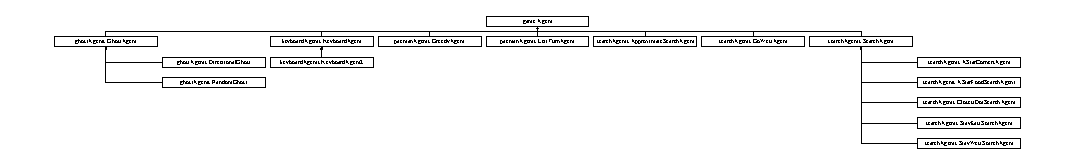
\includegraphics[height=1.770551cm]{classgame_1_1_agent}
\end{center}
\end{figure}
\subsection*{Public Member Functions}
\begin{DoxyCompactItemize}
\item 
\mbox{\Hypertarget{classgame_1_1_agent_aee5fbd6b9e05432c2d47051c516b9ae6}\label{classgame_1_1_agent_aee5fbd6b9e05432c2d47051c516b9ae6}} 
def {\bfseries \+\_\+\+\_\+init\+\_\+\+\_\+} (self, index=0)
\item 
def \hyperlink{classgame_1_1_agent_a6de8008ed3294dd312ecb45a32f63084}{get\+Action} (self, state)
\end{DoxyCompactItemize}
\subsection*{Public Attributes}
\begin{DoxyCompactItemize}
\item 
\mbox{\Hypertarget{classgame_1_1_agent_a171e9f5f634b834d4aa33c1120851235}\label{classgame_1_1_agent_a171e9f5f634b834d4aa33c1120851235}} 
{\bfseries index}
\end{DoxyCompactItemize}


\subsection{Detailed Description}
Parts worth reading \#. 

\begin{DoxyVerb}An agent must define a getAction method, but may also define the
following methods which will be called if they exist:

def registerInitialState(self, state): # inspects the starting state
\end{DoxyVerb}
 

\subsection{Member Function Documentation}
\mbox{\Hypertarget{classgame_1_1_agent_a6de8008ed3294dd312ecb45a32f63084}\label{classgame_1_1_agent_a6de8008ed3294dd312ecb45a32f63084}} 
\index{game\+::\+Agent@{game\+::\+Agent}!get\+Action@{get\+Action}}
\index{get\+Action@{get\+Action}!game\+::\+Agent@{game\+::\+Agent}}
\subsubsection{\texorpdfstring{get\+Action()}{getAction()}}
{\footnotesize\ttfamily def game.\+Agent.\+get\+Action (\begin{DoxyParamCaption}\item[{}]{self,  }\item[{}]{state }\end{DoxyParamCaption})}

\begin{DoxyVerb}The Agent will receive a GameState (from either {pacman, capture, sonar}.py) and
must return an action from Directions.{North, South, East, West, Stop}
\end{DoxyVerb}
 

The documentation for this class was generated from the following file\+:\begin{DoxyCompactItemize}
\item 
game.\+py\end{DoxyCompactItemize}

\hypertarget{classgame_1_1_agent_state}{}\section{game.\+Agent\+State Class Reference}
\label{classgame_1_1_agent_state}\index{game.\+Agent\+State@{game.\+Agent\+State}}
\subsection*{Public Member Functions}
\begin{DoxyCompactItemize}
\item 
\mbox{\Hypertarget{classgame_1_1_agent_state_ae766a9b7f726d3fefd66a1dd1d1a205b}\label{classgame_1_1_agent_state_ae766a9b7f726d3fefd66a1dd1d1a205b}} 
def {\bfseries \+\_\+\+\_\+init\+\_\+\+\_\+} (self, start\+Configuration, is\+Pacman)
\item 
\mbox{\Hypertarget{classgame_1_1_agent_state_a57b22b645dc8ea59d753482f941cadf4}\label{classgame_1_1_agent_state_a57b22b645dc8ea59d753482f941cadf4}} 
def {\bfseries \+\_\+\+\_\+str\+\_\+\+\_\+} (self)
\item 
\mbox{\Hypertarget{classgame_1_1_agent_state_a0152361046570e4adc1538bc80f5597d}\label{classgame_1_1_agent_state_a0152361046570e4adc1538bc80f5597d}} 
def {\bfseries \+\_\+\+\_\+eq\+\_\+\+\_\+} (self, other)
\item 
\mbox{\Hypertarget{classgame_1_1_agent_state_aceebe5bf82ab15a2dd41e68a0320b2d1}\label{classgame_1_1_agent_state_aceebe5bf82ab15a2dd41e68a0320b2d1}} 
def {\bfseries \+\_\+\+\_\+hash\+\_\+\+\_\+} (self)
\item 
\mbox{\Hypertarget{classgame_1_1_agent_state_a63ed2410fe71c9d86e7f1158ac270b16}\label{classgame_1_1_agent_state_a63ed2410fe71c9d86e7f1158ac270b16}} 
def {\bfseries copy} (self)
\item 
\mbox{\Hypertarget{classgame_1_1_agent_state_aa31ead4e3ff2fb8cd28264950567c970}\label{classgame_1_1_agent_state_aa31ead4e3ff2fb8cd28264950567c970}} 
def {\bfseries get\+Position} (self)
\item 
\mbox{\Hypertarget{classgame_1_1_agent_state_acf377ebf6704a25428a2c96737cb3071}\label{classgame_1_1_agent_state_acf377ebf6704a25428a2c96737cb3071}} 
def {\bfseries get\+Direction} (self)
\end{DoxyCompactItemize}
\subsection*{Public Attributes}
\begin{DoxyCompactItemize}
\item 
\mbox{\Hypertarget{classgame_1_1_agent_state_aababfd569db2af85389b4ed54ad114f4}\label{classgame_1_1_agent_state_aababfd569db2af85389b4ed54ad114f4}} 
{\bfseries start}
\item 
\mbox{\Hypertarget{classgame_1_1_agent_state_a39c0db462c50b0485549a14816ab438d}\label{classgame_1_1_agent_state_a39c0db462c50b0485549a14816ab438d}} 
{\bfseries configuration}
\item 
\mbox{\Hypertarget{classgame_1_1_agent_state_aed55d1014e05b62c652a484a3bb6416c}\label{classgame_1_1_agent_state_aed55d1014e05b62c652a484a3bb6416c}} 
{\bfseries is\+Pacman}
\item 
\mbox{\Hypertarget{classgame_1_1_agent_state_ab28305007f9be94841f7d0c938ab9d8c}\label{classgame_1_1_agent_state_ab28305007f9be94841f7d0c938ab9d8c}} 
{\bfseries scared\+Timer}
\end{DoxyCompactItemize}


\subsection{Detailed Description}
\begin{DoxyVerb}AgentStates hold the state of an agent (configuration, speed, scared, etc).
\end{DoxyVerb}
 

The documentation for this class was generated from the following file\+:\begin{DoxyCompactItemize}
\item 
game.\+py\end{DoxyCompactItemize}

\hypertarget{classsearch_agents_1_1_any_food_search_problem}{}\section{search\+Agents.\+Any\+Food\+Search\+Problem Class Reference}
\label{classsearch_agents_1_1_any_food_search_problem}\index{search\+Agents.\+Any\+Food\+Search\+Problem@{search\+Agents.\+Any\+Food\+Search\+Problem}}
Inheritance diagram for search\+Agents.\+Any\+Food\+Search\+Problem\+:\begin{figure}[H]
\begin{center}
\leavevmode
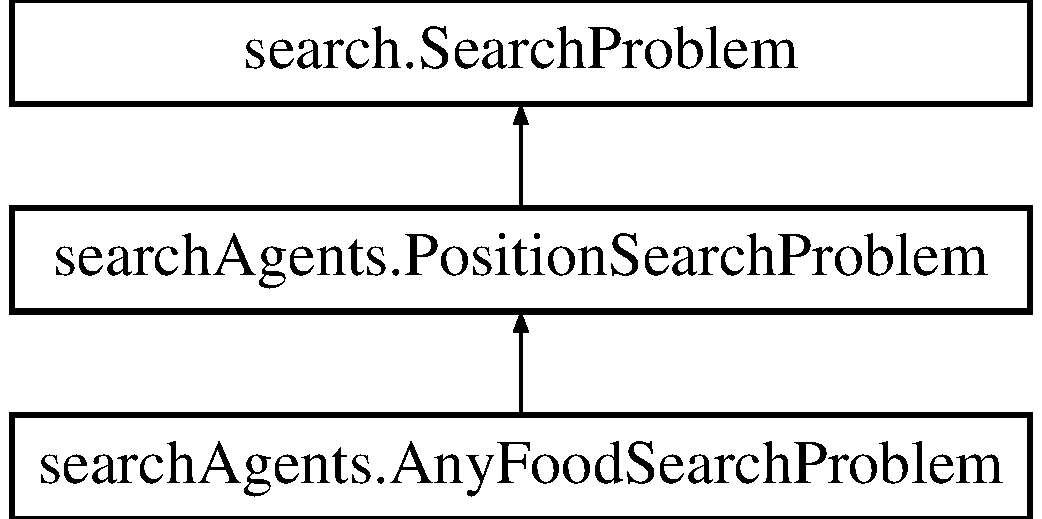
\includegraphics[height=3.000000cm]{classsearch_agents_1_1_any_food_search_problem}
\end{center}
\end{figure}
\subsection*{Public Member Functions}
\begin{DoxyCompactItemize}
\item 
\mbox{\Hypertarget{classsearch_agents_1_1_any_food_search_problem_a4d5a1064232c1ea9acb8e9d76580b225}\label{classsearch_agents_1_1_any_food_search_problem_a4d5a1064232c1ea9acb8e9d76580b225}} 
def {\bfseries \+\_\+\+\_\+init\+\_\+\+\_\+} (self, game\+State)
\item 
def \hyperlink{classsearch_agents_1_1_any_food_search_problem_a2b17e2e517592203930d4cc0ca29659a}{is\+Goal\+State} (self, state)
\end{DoxyCompactItemize}
\subsection*{Public Attributes}
\begin{DoxyCompactItemize}
\item 
\mbox{\Hypertarget{classsearch_agents_1_1_any_food_search_problem_aefcc56a1f0280214c66076fb9f86bc6c}\label{classsearch_agents_1_1_any_food_search_problem_aefcc56a1f0280214c66076fb9f86bc6c}} 
{\bfseries food}
\item 
\mbox{\Hypertarget{classsearch_agents_1_1_any_food_search_problem_aee38c772c21dd19790c052c6623aa9e8}\label{classsearch_agents_1_1_any_food_search_problem_aee38c772c21dd19790c052c6623aa9e8}} 
{\bfseries walls}
\item 
\mbox{\Hypertarget{classsearch_agents_1_1_any_food_search_problem_a4827bfdcd26355e9f66787338861c8b8}\label{classsearch_agents_1_1_any_food_search_problem_a4827bfdcd26355e9f66787338861c8b8}} 
{\bfseries start\+State}
\item 
\mbox{\Hypertarget{classsearch_agents_1_1_any_food_search_problem_abb374c075dafa0041e75e9f6700e2f93}\label{classsearch_agents_1_1_any_food_search_problem_abb374c075dafa0041e75e9f6700e2f93}} 
{\bfseries cost\+Fn}
\end{DoxyCompactItemize}


\subsection{Detailed Description}
\begin{DoxyVerb}  A search problem for finding a path to any food.

  This search problem is just like the PositionSearchProblem, but
  has a different goal test, which you need to fill in below.  The
  state space and successor function do not need to be changed.

  The class definition above, AnyFoodSearchProblem(PositionSearchProblem),
  inherits the methods of the PositionSearchProblem.

  You can use this search problem to help you fill in
  the findPathToClosestDot method.
\end{DoxyVerb}
 

\subsection{Member Function Documentation}
\mbox{\Hypertarget{classsearch_agents_1_1_any_food_search_problem_a2b17e2e517592203930d4cc0ca29659a}\label{classsearch_agents_1_1_any_food_search_problem_a2b17e2e517592203930d4cc0ca29659a}} 
\index{search\+Agents\+::\+Any\+Food\+Search\+Problem@{search\+Agents\+::\+Any\+Food\+Search\+Problem}!is\+Goal\+State@{is\+Goal\+State}}
\index{is\+Goal\+State@{is\+Goal\+State}!search\+Agents\+::\+Any\+Food\+Search\+Problem@{search\+Agents\+::\+Any\+Food\+Search\+Problem}}
\subsubsection{\texorpdfstring{is\+Goal\+State()}{isGoalState()}}
{\footnotesize\ttfamily def search\+Agents.\+Any\+Food\+Search\+Problem.\+is\+Goal\+State (\begin{DoxyParamCaption}\item[{}]{self,  }\item[{}]{state }\end{DoxyParamCaption})}

\begin{DoxyVerb}The state is Pacman's position. Fill this in with a goal test
that will complete the problem definition.
\end{DoxyVerb}
 

The documentation for this class was generated from the following file\+:\begin{DoxyCompactItemize}
\item 
search\+Agents.\+py\end{DoxyCompactItemize}

\hypertarget{classsearch_agents_1_1_approximate_search_agent}{}\section{search\+Agents.\+Approximate\+Search\+Agent Class Reference}
\label{classsearch_agents_1_1_approximate_search_agent}\index{search\+Agents.\+Approximate\+Search\+Agent@{search\+Agents.\+Approximate\+Search\+Agent}}
Inheritance diagram for search\+Agents.\+Approximate\+Search\+Agent\+:\begin{figure}[H]
\begin{center}
\leavevmode
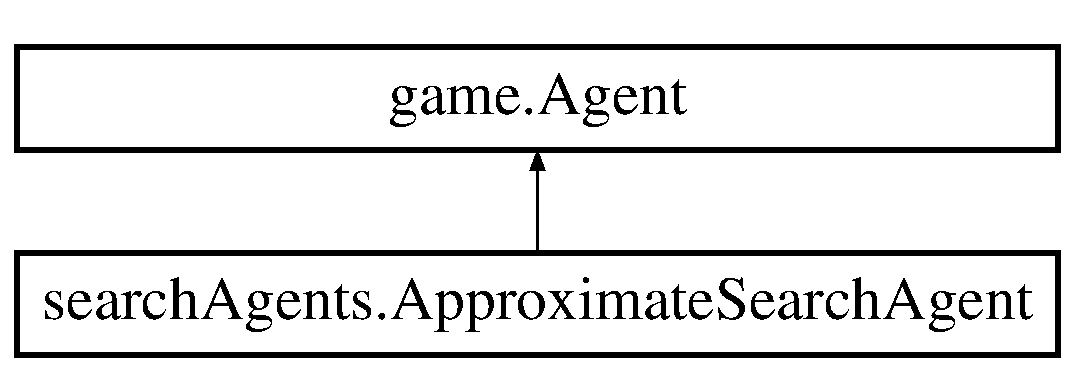
\includegraphics[height=2.000000cm]{classsearch_agents_1_1_approximate_search_agent}
\end{center}
\end{figure}
\subsection*{Public Member Functions}
\begin{DoxyCompactItemize}
\item 
\mbox{\Hypertarget{classsearch_agents_1_1_approximate_search_agent_ae8e395ee22a257e095c2b2d111670af3}\label{classsearch_agents_1_1_approximate_search_agent_ae8e395ee22a257e095c2b2d111670af3}} 
def {\bfseries register\+Initial\+State} (self, state)
\item 
def \hyperlink{classsearch_agents_1_1_approximate_search_agent_aade25c210785670dba8ee1e9a057f936}{get\+Action} (self, state)
\end{DoxyCompactItemize}
\subsection*{Additional Inherited Members}


\subsection{Member Function Documentation}
\mbox{\Hypertarget{classsearch_agents_1_1_approximate_search_agent_aade25c210785670dba8ee1e9a057f936}\label{classsearch_agents_1_1_approximate_search_agent_aade25c210785670dba8ee1e9a057f936}} 
\index{search\+Agents\+::\+Approximate\+Search\+Agent@{search\+Agents\+::\+Approximate\+Search\+Agent}!get\+Action@{get\+Action}}
\index{get\+Action@{get\+Action}!search\+Agents\+::\+Approximate\+Search\+Agent@{search\+Agents\+::\+Approximate\+Search\+Agent}}
\subsubsection{\texorpdfstring{get\+Action()}{getAction()}}
{\footnotesize\ttfamily def search\+Agents.\+Approximate\+Search\+Agent.\+get\+Action (\begin{DoxyParamCaption}\item[{}]{self,  }\item[{}]{state }\end{DoxyParamCaption})}

\begin{DoxyVerb}From game.py:
The Agent will receive a GameState and must return an action from
Directions.{North, South, East, West, Stop}
\end{DoxyVerb}
 

The documentation for this class was generated from the following file\+:\begin{DoxyCompactItemize}
\item 
search\+Agents.\+py\end{DoxyCompactItemize}

\hypertarget{classsearch_agents_1_1_a_star_corners_agent}{}\section{search\+Agents.\+A\+Star\+Corners\+Agent Class Reference}
\label{classsearch_agents_1_1_a_star_corners_agent}\index{search\+Agents.\+A\+Star\+Corners\+Agent@{search\+Agents.\+A\+Star\+Corners\+Agent}}
Inheritance diagram for search\+Agents.\+A\+Star\+Corners\+Agent\+:\begin{figure}[H]
\begin{center}
\leavevmode
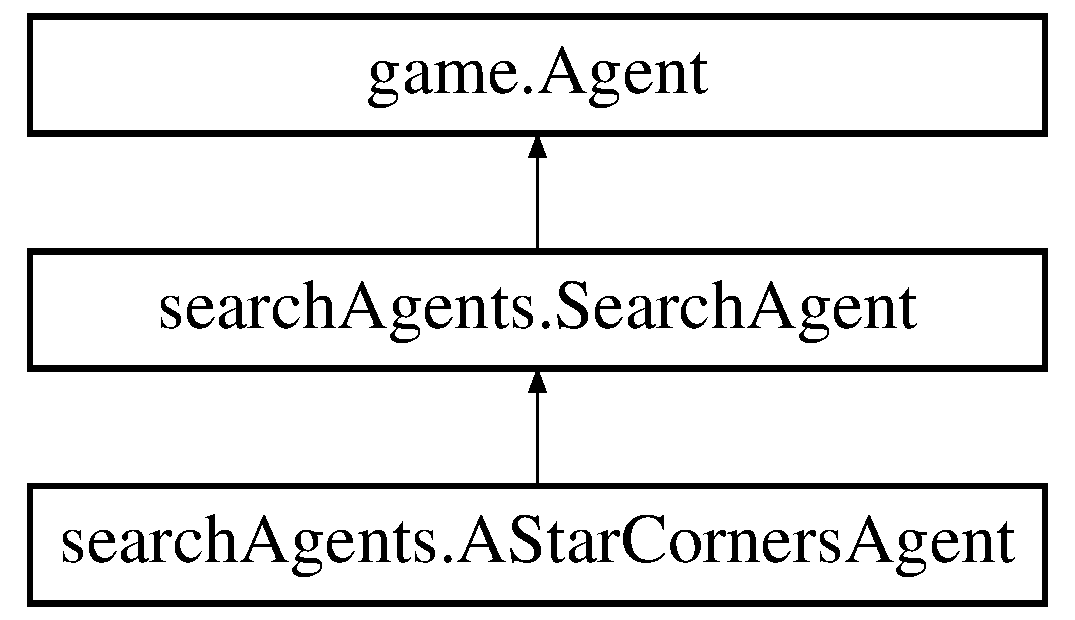
\includegraphics[height=3.000000cm]{classsearch_agents_1_1_a_star_corners_agent}
\end{center}
\end{figure}
\subsection*{Public Member Functions}
\begin{DoxyCompactItemize}
\item 
\mbox{\Hypertarget{classsearch_agents_1_1_a_star_corners_agent_af62eb95e3d237100325fa774514628e7}\label{classsearch_agents_1_1_a_star_corners_agent_af62eb95e3d237100325fa774514628e7}} 
def {\bfseries \+\_\+\+\_\+init\+\_\+\+\_\+} (self)
\end{DoxyCompactItemize}
\subsection*{Public Attributes}
\begin{DoxyCompactItemize}
\item 
\mbox{\Hypertarget{classsearch_agents_1_1_a_star_corners_agent_a8e5fb9dfc31d977e5f302c6e92523615}\label{classsearch_agents_1_1_a_star_corners_agent_a8e5fb9dfc31d977e5f302c6e92523615}} 
{\bfseries search\+Function}
\item 
\mbox{\Hypertarget{classsearch_agents_1_1_a_star_corners_agent_a340f07163c7ccea74ea2155bd6113e77}\label{classsearch_agents_1_1_a_star_corners_agent_a340f07163c7ccea74ea2155bd6113e77}} 
{\bfseries search\+Type}
\end{DoxyCompactItemize}


The documentation for this class was generated from the following file\+:\begin{DoxyCompactItemize}
\item 
search\+Agents.\+py\end{DoxyCompactItemize}

\hypertarget{classsearch_agents_1_1_a_star_food_search_agent}{}\section{search\+Agents.\+A\+Star\+Food\+Search\+Agent Class Reference}
\label{classsearch_agents_1_1_a_star_food_search_agent}\index{search\+Agents.\+A\+Star\+Food\+Search\+Agent@{search\+Agents.\+A\+Star\+Food\+Search\+Agent}}
Inheritance diagram for search\+Agents.\+A\+Star\+Food\+Search\+Agent\+:\begin{figure}[H]
\begin{center}
\leavevmode
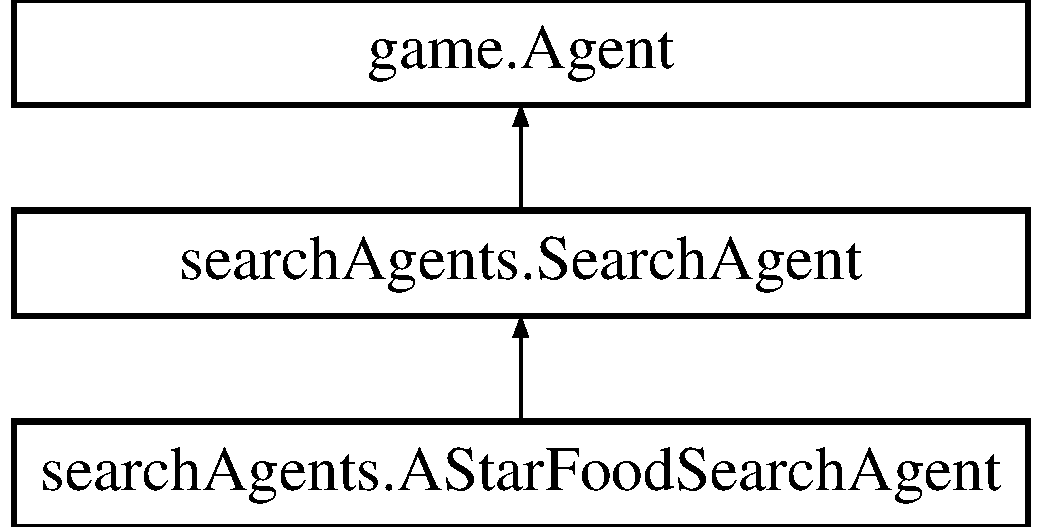
\includegraphics[height=3.000000cm]{classsearch_agents_1_1_a_star_food_search_agent}
\end{center}
\end{figure}
\subsection*{Public Member Functions}
\begin{DoxyCompactItemize}
\item 
\mbox{\Hypertarget{classsearch_agents_1_1_a_star_food_search_agent_a6cca432740051234c47d3a28273a8b4e}\label{classsearch_agents_1_1_a_star_food_search_agent_a6cca432740051234c47d3a28273a8b4e}} 
def {\bfseries \+\_\+\+\_\+init\+\_\+\+\_\+} (self)
\end{DoxyCompactItemize}
\subsection*{Public Attributes}
\begin{DoxyCompactItemize}
\item 
\mbox{\Hypertarget{classsearch_agents_1_1_a_star_food_search_agent_a54eeb36c41ecea572b931f8ffe93fbf0}\label{classsearch_agents_1_1_a_star_food_search_agent_a54eeb36c41ecea572b931f8ffe93fbf0}} 
{\bfseries search\+Function}
\item 
\mbox{\Hypertarget{classsearch_agents_1_1_a_star_food_search_agent_a8f93b1339dfc068a66e9f6eed2582fe2}\label{classsearch_agents_1_1_a_star_food_search_agent_a8f93b1339dfc068a66e9f6eed2582fe2}} 
{\bfseries search\+Type}
\end{DoxyCompactItemize}


The documentation for this class was generated from the following file\+:\begin{DoxyCompactItemize}
\item 
search\+Agents.\+py\end{DoxyCompactItemize}

\hypertarget{classpacman_1_1_classic_game_rules}{}\section{pacman.\+Classic\+Game\+Rules Class Reference}
\label{classpacman_1_1_classic_game_rules}\index{pacman.\+Classic\+Game\+Rules@{pacman.\+Classic\+Game\+Rules}}
\subsection*{Public Member Functions}
\begin{DoxyCompactItemize}
\item 
\mbox{\Hypertarget{classpacman_1_1_classic_game_rules_a545d789125db96710d31230ebf9d989c}\label{classpacman_1_1_classic_game_rules_a545d789125db96710d31230ebf9d989c}} 
def {\bfseries \+\_\+\+\_\+init\+\_\+\+\_\+} (self, timeout=30)
\item 
\mbox{\Hypertarget{classpacman_1_1_classic_game_rules_a19c2586ef3652dfd0f163270a1f030c2}\label{classpacman_1_1_classic_game_rules_a19c2586ef3652dfd0f163270a1f030c2}} 
def {\bfseries new\+Game} (self, layout, pacman\+Agent, ghost\+Agents, display, quiet=False, catch\+Exceptions=False)
\item 
def \hyperlink{classpacman_1_1_classic_game_rules_aa61bf270cf8e333d1aa805106afb08f9}{process} (self, state, game)
\item 
\mbox{\Hypertarget{classpacman_1_1_classic_game_rules_a04915c8a8ce4140b62e3304dd7fa1957}\label{classpacman_1_1_classic_game_rules_a04915c8a8ce4140b62e3304dd7fa1957}} 
def {\bfseries win} (self, state, game)
\item 
\mbox{\Hypertarget{classpacman_1_1_classic_game_rules_a7e16b67534a309cbdfb387df27647d84}\label{classpacman_1_1_classic_game_rules_a7e16b67534a309cbdfb387df27647d84}} 
def {\bfseries lose} (self, state, game)
\item 
\mbox{\Hypertarget{classpacman_1_1_classic_game_rules_aad38e1c704a99302196ad3d39fc5c7b7}\label{classpacman_1_1_classic_game_rules_aad38e1c704a99302196ad3d39fc5c7b7}} 
def {\bfseries get\+Progress} (self, game)
\item 
\mbox{\Hypertarget{classpacman_1_1_classic_game_rules_a4164536264d312b0412be9e944e40fa1}\label{classpacman_1_1_classic_game_rules_a4164536264d312b0412be9e944e40fa1}} 
def {\bfseries agent\+Crash} (self, game, agent\+Index)
\item 
\mbox{\Hypertarget{classpacman_1_1_classic_game_rules_a4cd03038895fae98ef88a87bd7021aa2}\label{classpacman_1_1_classic_game_rules_a4cd03038895fae98ef88a87bd7021aa2}} 
def {\bfseries get\+Max\+Total\+Time} (self, agent\+Index)
\item 
\mbox{\Hypertarget{classpacman_1_1_classic_game_rules_a99d3b445805e45d97f84c99d862db48d}\label{classpacman_1_1_classic_game_rules_a99d3b445805e45d97f84c99d862db48d}} 
def {\bfseries get\+Max\+Startup\+Time} (self, agent\+Index)
\item 
\mbox{\Hypertarget{classpacman_1_1_classic_game_rules_a77be77d83c6a3b61e089b1e6c68920f7}\label{classpacman_1_1_classic_game_rules_a77be77d83c6a3b61e089b1e6c68920f7}} 
def {\bfseries get\+Move\+Warning\+Time} (self, agent\+Index)
\item 
\mbox{\Hypertarget{classpacman_1_1_classic_game_rules_a37c5dccc853855827a6f0d4904466f4f}\label{classpacman_1_1_classic_game_rules_a37c5dccc853855827a6f0d4904466f4f}} 
def {\bfseries get\+Move\+Timeout} (self, agent\+Index)
\item 
\mbox{\Hypertarget{classpacman_1_1_classic_game_rules_a7a1d0b0a81c6187c8f5e0bc48c9f85fd}\label{classpacman_1_1_classic_game_rules_a7a1d0b0a81c6187c8f5e0bc48c9f85fd}} 
def {\bfseries get\+Max\+Time\+Warnings} (self, agent\+Index)
\end{DoxyCompactItemize}
\subsection*{Public Attributes}
\begin{DoxyCompactItemize}
\item 
\mbox{\Hypertarget{classpacman_1_1_classic_game_rules_a73cf20483aa9257e177ec3710e2a51f0}\label{classpacman_1_1_classic_game_rules_a73cf20483aa9257e177ec3710e2a51f0}} 
{\bfseries timeout}
\item 
\mbox{\Hypertarget{classpacman_1_1_classic_game_rules_a08305dede6923092ba2ffd280ae86eec}\label{classpacman_1_1_classic_game_rules_a08305dede6923092ba2ffd280ae86eec}} 
{\bfseries initial\+State}
\item 
\mbox{\Hypertarget{classpacman_1_1_classic_game_rules_ab66749219a7e83af074ced45d35b6073}\label{classpacman_1_1_classic_game_rules_ab66749219a7e83af074ced45d35b6073}} 
{\bfseries quiet}
\end{DoxyCompactItemize}


\subsection{Detailed Description}
\begin{DoxyVerb}These game rules manage the control flow of a game, deciding when
and how the game starts and ends.
\end{DoxyVerb}
 

\subsection{Member Function Documentation}
\mbox{\Hypertarget{classpacman_1_1_classic_game_rules_aa61bf270cf8e333d1aa805106afb08f9}\label{classpacman_1_1_classic_game_rules_aa61bf270cf8e333d1aa805106afb08f9}} 
\index{pacman\+::\+Classic\+Game\+Rules@{pacman\+::\+Classic\+Game\+Rules}!process@{process}}
\index{process@{process}!pacman\+::\+Classic\+Game\+Rules@{pacman\+::\+Classic\+Game\+Rules}}
\subsubsection{\texorpdfstring{process()}{process()}}
{\footnotesize\ttfamily def pacman.\+Classic\+Game\+Rules.\+process (\begin{DoxyParamCaption}\item[{}]{self,  }\item[{}]{state,  }\item[{}]{game }\end{DoxyParamCaption})}

\begin{DoxyVerb}Checks to see whether it is time to end the game.
\end{DoxyVerb}
 

The documentation for this class was generated from the following file\+:\begin{DoxyCompactItemize}
\item 
pacman.\+py\end{DoxyCompactItemize}

\hypertarget{classsearch_agents_1_1_closest_dot_search_agent}{}\section{search\+Agents.\+Closest\+Dot\+Search\+Agent Class Reference}
\label{classsearch_agents_1_1_closest_dot_search_agent}\index{search\+Agents.\+Closest\+Dot\+Search\+Agent@{search\+Agents.\+Closest\+Dot\+Search\+Agent}}
Inheritance diagram for search\+Agents.\+Closest\+Dot\+Search\+Agent\+:\begin{figure}[H]
\begin{center}
\leavevmode
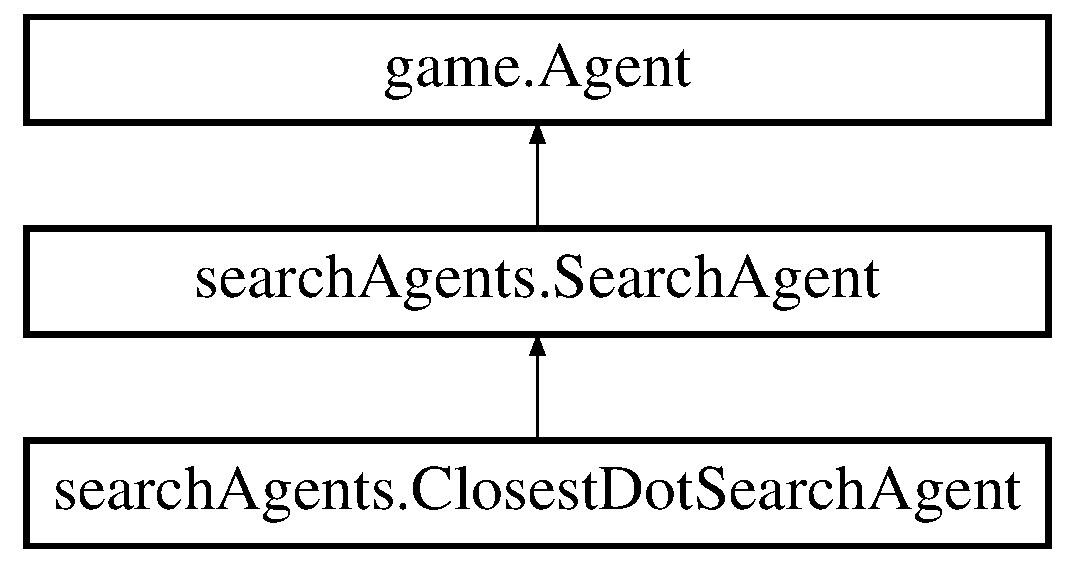
\includegraphics[height=3.000000cm]{classsearch_agents_1_1_closest_dot_search_agent}
\end{center}
\end{figure}
\subsection*{Public Member Functions}
\begin{DoxyCompactItemize}
\item 
\mbox{\Hypertarget{classsearch_agents_1_1_closest_dot_search_agent_aea2d09b148d9b56f9167139bf49d82d1}\label{classsearch_agents_1_1_closest_dot_search_agent_aea2d09b148d9b56f9167139bf49d82d1}} 
def {\bfseries register\+Initial\+State} (self, state)
\item 
\mbox{\Hypertarget{classsearch_agents_1_1_closest_dot_search_agent_a266dbaf93cf6709df5e7bcb083bf9911}\label{classsearch_agents_1_1_closest_dot_search_agent_a266dbaf93cf6709df5e7bcb083bf9911}} 
def {\bfseries find\+Path\+To\+Closest\+Dot} (self, game\+State)
\end{DoxyCompactItemize}
\subsection*{Public Attributes}
\begin{DoxyCompactItemize}
\item 
\mbox{\Hypertarget{classsearch_agents_1_1_closest_dot_search_agent_aac05cab3211d743d08adddecdf672ffd}\label{classsearch_agents_1_1_closest_dot_search_agent_aac05cab3211d743d08adddecdf672ffd}} 
{\bfseries actions}
\item 
\mbox{\Hypertarget{classsearch_agents_1_1_closest_dot_search_agent_a03bba84feac1d7c928042ca27db3b600}\label{classsearch_agents_1_1_closest_dot_search_agent_a03bba84feac1d7c928042ca27db3b600}} 
{\bfseries action\+Index}
\end{DoxyCompactItemize}


The documentation for this class was generated from the following file\+:\begin{DoxyCompactItemize}
\item 
search\+Agents.\+py\end{DoxyCompactItemize}

\hypertarget{classgame_1_1_configuration}{}\section{game.\+Configuration Class Reference}
\label{classgame_1_1_configuration}\index{game.\+Configuration@{game.\+Configuration}}
\subsection*{Public Member Functions}
\begin{DoxyCompactItemize}
\item 
\mbox{\Hypertarget{classgame_1_1_configuration_a09f875cab5e96bc903e5390b6742eb03}\label{classgame_1_1_configuration_a09f875cab5e96bc903e5390b6742eb03}} 
def {\bfseries \+\_\+\+\_\+init\+\_\+\+\_\+} (self, pos, direction)
\item 
\mbox{\Hypertarget{classgame_1_1_configuration_a2b56d29c113daa2c2f6684a777192dff}\label{classgame_1_1_configuration_a2b56d29c113daa2c2f6684a777192dff}} 
def {\bfseries get\+Position} (self)
\item 
\mbox{\Hypertarget{classgame_1_1_configuration_a3e510d8e5104e13681f2c5f066a86b71}\label{classgame_1_1_configuration_a3e510d8e5104e13681f2c5f066a86b71}} 
def {\bfseries get\+Direction} (self)
\item 
\mbox{\Hypertarget{classgame_1_1_configuration_ac3e5734175aaf38e7e766c29d99a7997}\label{classgame_1_1_configuration_ac3e5734175aaf38e7e766c29d99a7997}} 
def {\bfseries is\+Integer} (self)
\item 
\mbox{\Hypertarget{classgame_1_1_configuration_afda2e6acf77361ede5b64b76097db7c4}\label{classgame_1_1_configuration_afda2e6acf77361ede5b64b76097db7c4}} 
def {\bfseries \+\_\+\+\_\+eq\+\_\+\+\_\+} (self, other)
\item 
\mbox{\Hypertarget{classgame_1_1_configuration_a093f183229637e1de2cd36dfa3ca6968}\label{classgame_1_1_configuration_a093f183229637e1de2cd36dfa3ca6968}} 
def {\bfseries \+\_\+\+\_\+hash\+\_\+\+\_\+} (self)
\item 
\mbox{\Hypertarget{classgame_1_1_configuration_a900303f94f3f07e67f80df913282dd7a}\label{classgame_1_1_configuration_a900303f94f3f07e67f80df913282dd7a}} 
def {\bfseries \+\_\+\+\_\+str\+\_\+\+\_\+} (self)
\item 
def \hyperlink{classgame_1_1_configuration_a282e5131bfdb055bdddde8df6d881c02}{generate\+Successor} (self, vector)
\end{DoxyCompactItemize}
\subsection*{Public Attributes}
\begin{DoxyCompactItemize}
\item 
\mbox{\Hypertarget{classgame_1_1_configuration_a152722015a1e6841fd840c7143285dfe}\label{classgame_1_1_configuration_a152722015a1e6841fd840c7143285dfe}} 
{\bfseries pos}
\item 
\mbox{\Hypertarget{classgame_1_1_configuration_a9e623b37d8b98a775937b1f65fedf783}\label{classgame_1_1_configuration_a9e623b37d8b98a775937b1f65fedf783}} 
{\bfseries direction}
\end{DoxyCompactItemize}


\subsection{Detailed Description}
\begin{DoxyVerb}A Configuration holds the (x,y) coordinate of a character, along with its
traveling direction.

The convention for positions, like a graph, is that (0,0) is the lower left corner, x increases
horizontally and y increases vertically.  Therefore, north is the direction of increasing y, or (0,1).
\end{DoxyVerb}
 

\subsection{Member Function Documentation}
\mbox{\Hypertarget{classgame_1_1_configuration_a282e5131bfdb055bdddde8df6d881c02}\label{classgame_1_1_configuration_a282e5131bfdb055bdddde8df6d881c02}} 
\index{game\+::\+Configuration@{game\+::\+Configuration}!generate\+Successor@{generate\+Successor}}
\index{generate\+Successor@{generate\+Successor}!game\+::\+Configuration@{game\+::\+Configuration}}
\subsubsection{\texorpdfstring{generate\+Successor()}{generateSuccessor()}}
{\footnotesize\ttfamily def game.\+Configuration.\+generate\+Successor (\begin{DoxyParamCaption}\item[{}]{self,  }\item[{}]{vector }\end{DoxyParamCaption})}

\begin{DoxyVerb}Generates a new configuration reached by translating the current
configuration by the action vector.  This is a low-level call and does
not attempt to respect the legality of the movement.

Actions are movement vectors.
\end{DoxyVerb}
 

The documentation for this class was generated from the following file\+:\begin{DoxyCompactItemize}
\item 
game.\+py\end{DoxyCompactItemize}

\hypertarget{classsearch_agents_1_1_corners_problem}{}\section{search\+Agents.\+Corners\+Problem Class Reference}
\label{classsearch_agents_1_1_corners_problem}\index{search\+Agents.\+Corners\+Problem@{search\+Agents.\+Corners\+Problem}}


This portion is incomplete.  


Inheritance diagram for search\+Agents.\+Corners\+Problem\+:\begin{figure}[H]
\begin{center}
\leavevmode
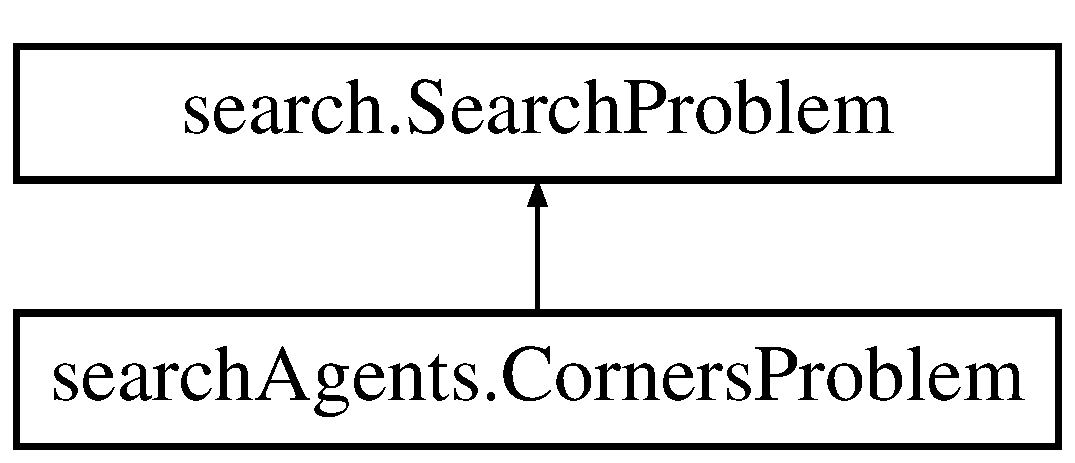
\includegraphics[height=2.000000cm]{classsearch_agents_1_1_corners_problem}
\end{center}
\end{figure}
\subsection*{Public Member Functions}
\begin{DoxyCompactItemize}
\item 
def \hyperlink{classsearch_agents_1_1_corners_problem_a8f0a2bae690d6d0ee6ddb6515ef477d9}{\+\_\+\+\_\+init\+\_\+\+\_\+} (self, starting\+Game\+State)
\item 
\mbox{\Hypertarget{classsearch_agents_1_1_corners_problem_a977edf899a044c6c6dfb10912511c111}\label{classsearch_agents_1_1_corners_problem_a977edf899a044c6c6dfb10912511c111}} 
def {\bfseries get\+Start\+State} (self)
\item 
\mbox{\Hypertarget{classsearch_agents_1_1_corners_problem_a73266786a18f9064a72dacbca62d88f5}\label{classsearch_agents_1_1_corners_problem_a73266786a18f9064a72dacbca62d88f5}} 
def {\bfseries is\+Goal\+State} (self, state)
\item 
def \hyperlink{classsearch_agents_1_1_corners_problem_a9f612b359d4cd90ff87759c4ade8fbab}{get\+Successors} (self, state)
\item 
def \hyperlink{classsearch_agents_1_1_corners_problem_a0530021a28c4f2e26866761ece75cec8}{get\+Cost\+Of\+Actions} (self, actions)
\end{DoxyCompactItemize}
\subsection*{Public Attributes}
\begin{DoxyCompactItemize}
\item 
\mbox{\Hypertarget{classsearch_agents_1_1_corners_problem_a7afbc50121078e7ee8e67e6c5b4871e9}\label{classsearch_agents_1_1_corners_problem_a7afbc50121078e7ee8e67e6c5b4871e9}} 
{\bfseries walls}
\item 
\mbox{\Hypertarget{classsearch_agents_1_1_corners_problem_a8b95bc921aa406bbd5aa8249aa73f932}\label{classsearch_agents_1_1_corners_problem_a8b95bc921aa406bbd5aa8249aa73f932}} 
{\bfseries starting\+Position}
\item 
\mbox{\Hypertarget{classsearch_agents_1_1_corners_problem_a3a92389a3705e5feac95cb72d8e681aa}\label{classsearch_agents_1_1_corners_problem_a3a92389a3705e5feac95cb72d8e681aa}} 
{\bfseries corners}
\end{DoxyCompactItemize}


\subsection{Detailed Description}
This portion is incomplete. 

Time to write code! \#\begin{DoxyVerb}This search problem finds paths through all four corners of a layout.

You must select a suitable state space and successor function
\end{DoxyVerb}
 

\subsection{Constructor \& Destructor Documentation}
\mbox{\Hypertarget{classsearch_agents_1_1_corners_problem_a8f0a2bae690d6d0ee6ddb6515ef477d9}\label{classsearch_agents_1_1_corners_problem_a8f0a2bae690d6d0ee6ddb6515ef477d9}} 
\index{search\+Agents\+::\+Corners\+Problem@{search\+Agents\+::\+Corners\+Problem}!\+\_\+\+\_\+init\+\_\+\+\_\+@{\+\_\+\+\_\+init\+\_\+\+\_\+}}
\index{\+\_\+\+\_\+init\+\_\+\+\_\+@{\+\_\+\+\_\+init\+\_\+\+\_\+}!search\+Agents\+::\+Corners\+Problem@{search\+Agents\+::\+Corners\+Problem}}
\subsubsection{\texorpdfstring{\+\_\+\+\_\+init\+\_\+\+\_\+()}{\_\_init\_\_()}}
{\footnotesize\ttfamily def search\+Agents.\+Corners\+Problem.\+\_\+\+\_\+init\+\_\+\+\_\+ (\begin{DoxyParamCaption}\item[{}]{self,  }\item[{}]{starting\+Game\+State }\end{DoxyParamCaption})}

\begin{DoxyVerb}Stores the walls, pacman's starting position and corners.
\end{DoxyVerb}
 

\subsection{Member Function Documentation}
\mbox{\Hypertarget{classsearch_agents_1_1_corners_problem_a0530021a28c4f2e26866761ece75cec8}\label{classsearch_agents_1_1_corners_problem_a0530021a28c4f2e26866761ece75cec8}} 
\index{search\+Agents\+::\+Corners\+Problem@{search\+Agents\+::\+Corners\+Problem}!get\+Cost\+Of\+Actions@{get\+Cost\+Of\+Actions}}
\index{get\+Cost\+Of\+Actions@{get\+Cost\+Of\+Actions}!search\+Agents\+::\+Corners\+Problem@{search\+Agents\+::\+Corners\+Problem}}
\subsubsection{\texorpdfstring{get\+Cost\+Of\+Actions()}{getCostOfActions()}}
{\footnotesize\ttfamily def search\+Agents.\+Corners\+Problem.\+get\+Cost\+Of\+Actions (\begin{DoxyParamCaption}\item[{}]{self,  }\item[{}]{actions }\end{DoxyParamCaption})}

\begin{DoxyVerb}Returns the cost of a particular sequence of actions.  If those actions
include an illegal move, return 999999.  This is implemented for you.
\end{DoxyVerb}
 \mbox{\Hypertarget{classsearch_agents_1_1_corners_problem_a9f612b359d4cd90ff87759c4ade8fbab}\label{classsearch_agents_1_1_corners_problem_a9f612b359d4cd90ff87759c4ade8fbab}} 
\index{search\+Agents\+::\+Corners\+Problem@{search\+Agents\+::\+Corners\+Problem}!get\+Successors@{get\+Successors}}
\index{get\+Successors@{get\+Successors}!search\+Agents\+::\+Corners\+Problem@{search\+Agents\+::\+Corners\+Problem}}
\subsubsection{\texorpdfstring{get\+Successors()}{getSuccessors()}}
{\footnotesize\ttfamily def search\+Agents.\+Corners\+Problem.\+get\+Successors (\begin{DoxyParamCaption}\item[{}]{self,  }\item[{}]{state }\end{DoxyParamCaption})}

\begin{DoxyVerb}Returns successor states, the actions they require, and a cost of 1.

 As noted in search.py:
     For a given state, this should return a list of triples,
 (successor, action, stepCost), where 'successor' is a
 successor to the current state, 'action' is the action
 required to get there, and 'stepCost' is the incremental
 cost of expanding to that successor
\end{DoxyVerb}
 

The documentation for this class was generated from the following file\+:\begin{DoxyCompactItemize}
\item 
search\+Agents.\+py\end{DoxyCompactItemize}

\hypertarget{classutil_1_1_counter}{}\section{util.\+Counter Class Reference}
\label{classutil_1_1_counter}\index{util.\+Counter@{util.\+Counter}}
Inheritance diagram for util.\+Counter\+:\begin{figure}[H]
\begin{center}
\leavevmode
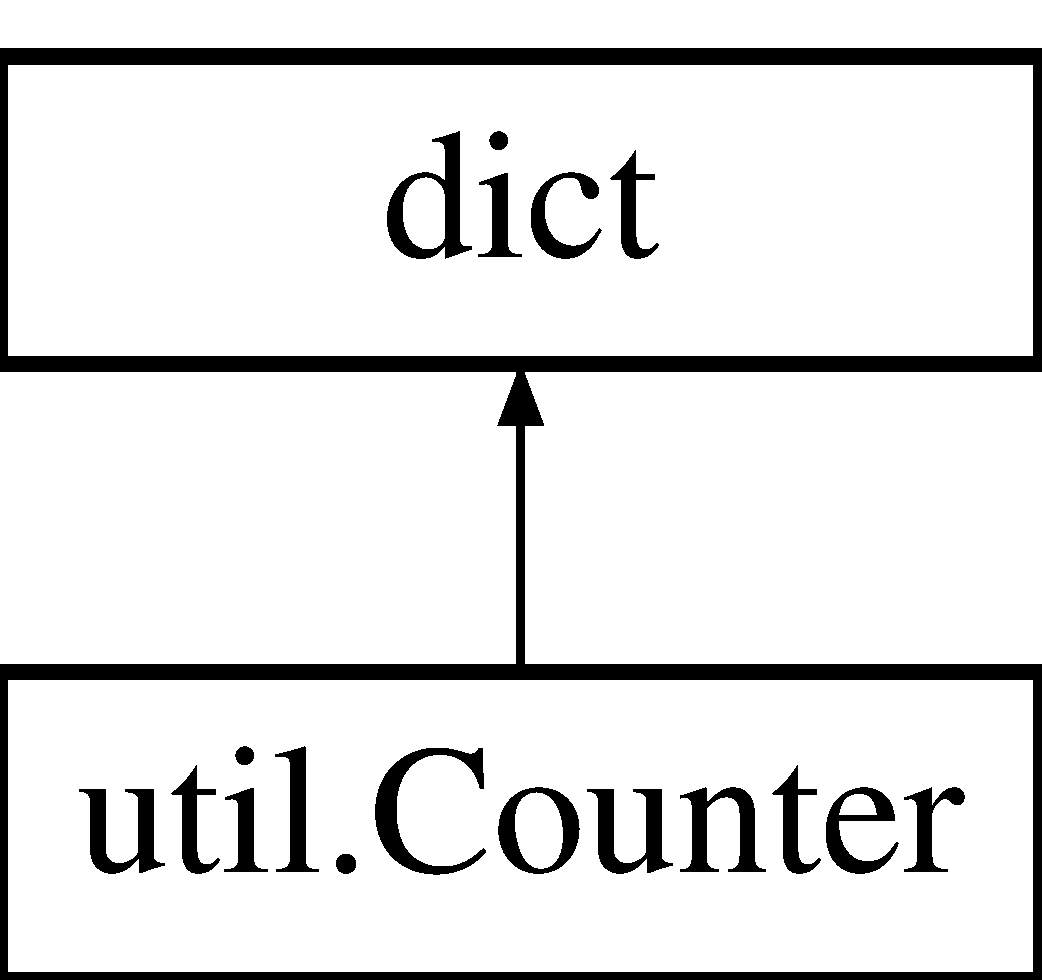
\includegraphics[height=2.000000cm]{classutil_1_1_counter}
\end{center}
\end{figure}
\subsection*{Public Member Functions}
\begin{DoxyCompactItemize}
\item 
\mbox{\Hypertarget{classutil_1_1_counter_a5adf33996410dfdeddfdb4d6d600a587}\label{classutil_1_1_counter_a5adf33996410dfdeddfdb4d6d600a587}} 
def {\bfseries \+\_\+\+\_\+getitem\+\_\+\+\_\+} (self, idx)
\item 
def \hyperlink{classutil_1_1_counter_a92c9ebbb536e6febb2b2856f30f21804}{increment\+All} (self, keys, count)
\item 
def \hyperlink{classutil_1_1_counter_ac783df5e03c63469983b812fd5aff0c2}{arg\+Max} (self)
\item 
def \hyperlink{classutil_1_1_counter_a8e32d106f34cb7cd8341e78b49f5e40a}{sorted\+Keys} (self)
\item 
def \hyperlink{classutil_1_1_counter_a452a24a68fa547c7bf56e619be6bab6d}{total\+Count} (self)
\item 
def \hyperlink{classutil_1_1_counter_a5d3243989dde93af492d2a7618ea322f}{normalize} (self)
\item 
def \hyperlink{classutil_1_1_counter_a510574fa4c36d2d4c845b9f6ac5bc155}{divide\+All} (self, divisor)
\item 
def \hyperlink{classutil_1_1_counter_ac57004446c3d5a15948e7803a0af3d56}{copy} (self)
\item 
def \hyperlink{classutil_1_1_counter_a9f43e857acc90d489555652af32dcd1c}{\+\_\+\+\_\+mul\+\_\+\+\_\+} (self, y)
\item 
def \hyperlink{classutil_1_1_counter_a4d15b474f84349a6d6b0694066b16ac2}{\+\_\+\+\_\+radd\+\_\+\+\_\+} (self, y)
\item 
def \hyperlink{classutil_1_1_counter_ac9dfb7fe386dc63f8d27a66984d5bc75}{\+\_\+\+\_\+add\+\_\+\+\_\+} (self, y)
\item 
def \hyperlink{classutil_1_1_counter_a541fd5f4f74e910852c589ff23b4b280}{\+\_\+\+\_\+sub\+\_\+\+\_\+} (self, y)
\end{DoxyCompactItemize}


\subsection{Detailed Description}
\begin{DoxyVerb}A counter keeps track of counts for a set of keys.

The counter class is an extension of the standard python
dictionary type.  It is specialized to have number values  
(integers or floats), and includes a handful of additional
functions to ease the task of counting data.  In particular, 
all keys are defaulted to have value 0.  Using a dictionary:

a = {}
print a['test']

would give an error, while the Counter class analogue:
  
>>> a = Counter()
>>> print a['test']
0

returns the default 0 value. Note that to reference a key 
that you know is contained in the counter, 
you can still use the dictionary syntax:
  
>>> a = Counter()
>>> a['test'] = 2
>>> print a['test']
2

This is very useful for counting things without initializing their counts,
see for example:

>>> a['blah'] += 1
>>> print a['blah']
1

The counter also includes additional functionality useful in implementing
the classifiers for this assignment.  Two counters can be added,
subtracted or multiplied together.  See below for details.  They can
also be normalized and their total count and arg max can be extracted.
\end{DoxyVerb}
 

\subsection{Member Function Documentation}
\mbox{\Hypertarget{classutil_1_1_counter_ac9dfb7fe386dc63f8d27a66984d5bc75}\label{classutil_1_1_counter_ac9dfb7fe386dc63f8d27a66984d5bc75}} 
\index{util\+::\+Counter@{util\+::\+Counter}!\+\_\+\+\_\+add\+\_\+\+\_\+@{\+\_\+\+\_\+add\+\_\+\+\_\+}}
\index{\+\_\+\+\_\+add\+\_\+\+\_\+@{\+\_\+\+\_\+add\+\_\+\+\_\+}!util\+::\+Counter@{util\+::\+Counter}}
\subsubsection{\texorpdfstring{\+\_\+\+\_\+add\+\_\+\+\_\+()}{\_\_add\_\_()}}
{\footnotesize\ttfamily def util.\+Counter.\+\_\+\+\_\+add\+\_\+\+\_\+ (\begin{DoxyParamCaption}\item[{}]{self,  }\item[{}]{y }\end{DoxyParamCaption})}

\begin{DoxyVerb}Adding two counters gives a counter with the union of all keys and
counts of the second added to counts of the first.

>>> a = Counter()
>>> b = Counter()
>>> a['first'] = -2
>>> a['second'] = 4
>>> b['first'] = 3
>>> b['third'] = 1
>>> (a + b)['first']
1
\end{DoxyVerb}
 \mbox{\Hypertarget{classutil_1_1_counter_a9f43e857acc90d489555652af32dcd1c}\label{classutil_1_1_counter_a9f43e857acc90d489555652af32dcd1c}} 
\index{util\+::\+Counter@{util\+::\+Counter}!\+\_\+\+\_\+mul\+\_\+\+\_\+@{\+\_\+\+\_\+mul\+\_\+\+\_\+}}
\index{\+\_\+\+\_\+mul\+\_\+\+\_\+@{\+\_\+\+\_\+mul\+\_\+\+\_\+}!util\+::\+Counter@{util\+::\+Counter}}
\subsubsection{\texorpdfstring{\+\_\+\+\_\+mul\+\_\+\+\_\+()}{\_\_mul\_\_()}}
{\footnotesize\ttfamily def util.\+Counter.\+\_\+\+\_\+mul\+\_\+\+\_\+ (\begin{DoxyParamCaption}\item[{}]{self,  }\item[{}]{y }\end{DoxyParamCaption})}

\begin{DoxyVerb}Multiplying two counters gives the dot product of their vectors where
each unique label is a vector element.

>>> a = Counter()
>>> b = Counter()
>>> a['first'] = -2
>>> a['second'] = 4
>>> b['first'] = 3
>>> b['second'] = 5
>>> a['third'] = 1.5
>>> a['fourth'] = 2.5
>>> a * b
14
\end{DoxyVerb}
 \mbox{\Hypertarget{classutil_1_1_counter_a4d15b474f84349a6d6b0694066b16ac2}\label{classutil_1_1_counter_a4d15b474f84349a6d6b0694066b16ac2}} 
\index{util\+::\+Counter@{util\+::\+Counter}!\+\_\+\+\_\+radd\+\_\+\+\_\+@{\+\_\+\+\_\+radd\+\_\+\+\_\+}}
\index{\+\_\+\+\_\+radd\+\_\+\+\_\+@{\+\_\+\+\_\+radd\+\_\+\+\_\+}!util\+::\+Counter@{util\+::\+Counter}}
\subsubsection{\texorpdfstring{\+\_\+\+\_\+radd\+\_\+\+\_\+()}{\_\_radd\_\_()}}
{\footnotesize\ttfamily def util.\+Counter.\+\_\+\+\_\+radd\+\_\+\+\_\+ (\begin{DoxyParamCaption}\item[{}]{self,  }\item[{}]{y }\end{DoxyParamCaption})}

\begin{DoxyVerb}Adding another counter to a counter increments the current counter
by the values stored in the second counter.

>>> a = Counter()
>>> b = Counter()
>>> a['first'] = -2
>>> a['second'] = 4
>>> b['first'] = 3
>>> b['third'] = 1
>>> a += b
>>> a['first']
1
\end{DoxyVerb}
 \mbox{\Hypertarget{classutil_1_1_counter_a541fd5f4f74e910852c589ff23b4b280}\label{classutil_1_1_counter_a541fd5f4f74e910852c589ff23b4b280}} 
\index{util\+::\+Counter@{util\+::\+Counter}!\+\_\+\+\_\+sub\+\_\+\+\_\+@{\+\_\+\+\_\+sub\+\_\+\+\_\+}}
\index{\+\_\+\+\_\+sub\+\_\+\+\_\+@{\+\_\+\+\_\+sub\+\_\+\+\_\+}!util\+::\+Counter@{util\+::\+Counter}}
\subsubsection{\texorpdfstring{\+\_\+\+\_\+sub\+\_\+\+\_\+()}{\_\_sub\_\_()}}
{\footnotesize\ttfamily def util.\+Counter.\+\_\+\+\_\+sub\+\_\+\+\_\+ (\begin{DoxyParamCaption}\item[{}]{self,  }\item[{}]{y }\end{DoxyParamCaption})}

\begin{DoxyVerb}Subtracting a counter from another gives a counter with the union of all keys and
counts of the second subtracted from counts of the first.

>>> a = Counter()
>>> b = Counter()
>>> a['first'] = -2
>>> a['second'] = 4
>>> b['first'] = 3
>>> b['third'] = 1
>>> (a - b)['first']
-5
\end{DoxyVerb}
 \mbox{\Hypertarget{classutil_1_1_counter_ac783df5e03c63469983b812fd5aff0c2}\label{classutil_1_1_counter_ac783df5e03c63469983b812fd5aff0c2}} 
\index{util\+::\+Counter@{util\+::\+Counter}!arg\+Max@{arg\+Max}}
\index{arg\+Max@{arg\+Max}!util\+::\+Counter@{util\+::\+Counter}}
\subsubsection{\texorpdfstring{arg\+Max()}{argMax()}}
{\footnotesize\ttfamily def util.\+Counter.\+arg\+Max (\begin{DoxyParamCaption}\item[{}]{self }\end{DoxyParamCaption})}

\begin{DoxyVerb}Returns the key with the highest value.
\end{DoxyVerb}
 \mbox{\Hypertarget{classutil_1_1_counter_ac57004446c3d5a15948e7803a0af3d56}\label{classutil_1_1_counter_ac57004446c3d5a15948e7803a0af3d56}} 
\index{util\+::\+Counter@{util\+::\+Counter}!copy@{copy}}
\index{copy@{copy}!util\+::\+Counter@{util\+::\+Counter}}
\subsubsection{\texorpdfstring{copy()}{copy()}}
{\footnotesize\ttfamily def util.\+Counter.\+copy (\begin{DoxyParamCaption}\item[{}]{self }\end{DoxyParamCaption})}

\begin{DoxyVerb}Returns a copy of the counter
\end{DoxyVerb}
 \mbox{\Hypertarget{classutil_1_1_counter_a510574fa4c36d2d4c845b9f6ac5bc155}\label{classutil_1_1_counter_a510574fa4c36d2d4c845b9f6ac5bc155}} 
\index{util\+::\+Counter@{util\+::\+Counter}!divide\+All@{divide\+All}}
\index{divide\+All@{divide\+All}!util\+::\+Counter@{util\+::\+Counter}}
\subsubsection{\texorpdfstring{divide\+All()}{divideAll()}}
{\footnotesize\ttfamily def util.\+Counter.\+divide\+All (\begin{DoxyParamCaption}\item[{}]{self,  }\item[{}]{divisor }\end{DoxyParamCaption})}

\begin{DoxyVerb}Divides all counts by divisor
\end{DoxyVerb}
 \mbox{\Hypertarget{classutil_1_1_counter_a92c9ebbb536e6febb2b2856f30f21804}\label{classutil_1_1_counter_a92c9ebbb536e6febb2b2856f30f21804}} 
\index{util\+::\+Counter@{util\+::\+Counter}!increment\+All@{increment\+All}}
\index{increment\+All@{increment\+All}!util\+::\+Counter@{util\+::\+Counter}}
\subsubsection{\texorpdfstring{increment\+All()}{incrementAll()}}
{\footnotesize\ttfamily def util.\+Counter.\+increment\+All (\begin{DoxyParamCaption}\item[{}]{self,  }\item[{}]{keys,  }\item[{}]{count }\end{DoxyParamCaption})}

\begin{DoxyVerb}Increments all elements of keys by the same count.

>>> a = Counter()
>>> a.incrementAll(['one','two', 'three'], 1)
>>> a['one']
1
>>> a['two']
1
\end{DoxyVerb}
 \mbox{\Hypertarget{classutil_1_1_counter_a5d3243989dde93af492d2a7618ea322f}\label{classutil_1_1_counter_a5d3243989dde93af492d2a7618ea322f}} 
\index{util\+::\+Counter@{util\+::\+Counter}!normalize@{normalize}}
\index{normalize@{normalize}!util\+::\+Counter@{util\+::\+Counter}}
\subsubsection{\texorpdfstring{normalize()}{normalize()}}
{\footnotesize\ttfamily def util.\+Counter.\+normalize (\begin{DoxyParamCaption}\item[{}]{self }\end{DoxyParamCaption})}

\begin{DoxyVerb}Edits the counter such that the total count of all
keys sums to 1.  The ratio of counts for all keys
will remain the same. Note that normalizing an empty 
Counter will result in an error.
\end{DoxyVerb}
 \mbox{\Hypertarget{classutil_1_1_counter_a8e32d106f34cb7cd8341e78b49f5e40a}\label{classutil_1_1_counter_a8e32d106f34cb7cd8341e78b49f5e40a}} 
\index{util\+::\+Counter@{util\+::\+Counter}!sorted\+Keys@{sorted\+Keys}}
\index{sorted\+Keys@{sorted\+Keys}!util\+::\+Counter@{util\+::\+Counter}}
\subsubsection{\texorpdfstring{sorted\+Keys()}{sortedKeys()}}
{\footnotesize\ttfamily def util.\+Counter.\+sorted\+Keys (\begin{DoxyParamCaption}\item[{}]{self }\end{DoxyParamCaption})}

\begin{DoxyVerb}Returns a list of keys sorted by their values.  Keys
with the highest values will appear first.

>>> a = Counter()
>>> a['first'] = -2
>>> a['second'] = 4
>>> a['third'] = 1
>>> a.sortedKeys()
['second', 'third', 'first']
\end{DoxyVerb}
 \mbox{\Hypertarget{classutil_1_1_counter_a452a24a68fa547c7bf56e619be6bab6d}\label{classutil_1_1_counter_a452a24a68fa547c7bf56e619be6bab6d}} 
\index{util\+::\+Counter@{util\+::\+Counter}!total\+Count@{total\+Count}}
\index{total\+Count@{total\+Count}!util\+::\+Counter@{util\+::\+Counter}}
\subsubsection{\texorpdfstring{total\+Count()}{totalCount()}}
{\footnotesize\ttfamily def util.\+Counter.\+total\+Count (\begin{DoxyParamCaption}\item[{}]{self }\end{DoxyParamCaption})}

\begin{DoxyVerb}Returns the sum of counts for all keys.
\end{DoxyVerb}
 

The documentation for this class was generated from the following file\+:\begin{DoxyCompactItemize}
\item 
util.\+py\end{DoxyCompactItemize}

\hypertarget{classghost_agents_1_1_directional_ghost}{}\section{ghost\+Agents.\+Directional\+Ghost Class Reference}
\label{classghost_agents_1_1_directional_ghost}\index{ghost\+Agents.\+Directional\+Ghost@{ghost\+Agents.\+Directional\+Ghost}}
Inheritance diagram for ghost\+Agents.\+Directional\+Ghost\+:\begin{figure}[H]
\begin{center}
\leavevmode
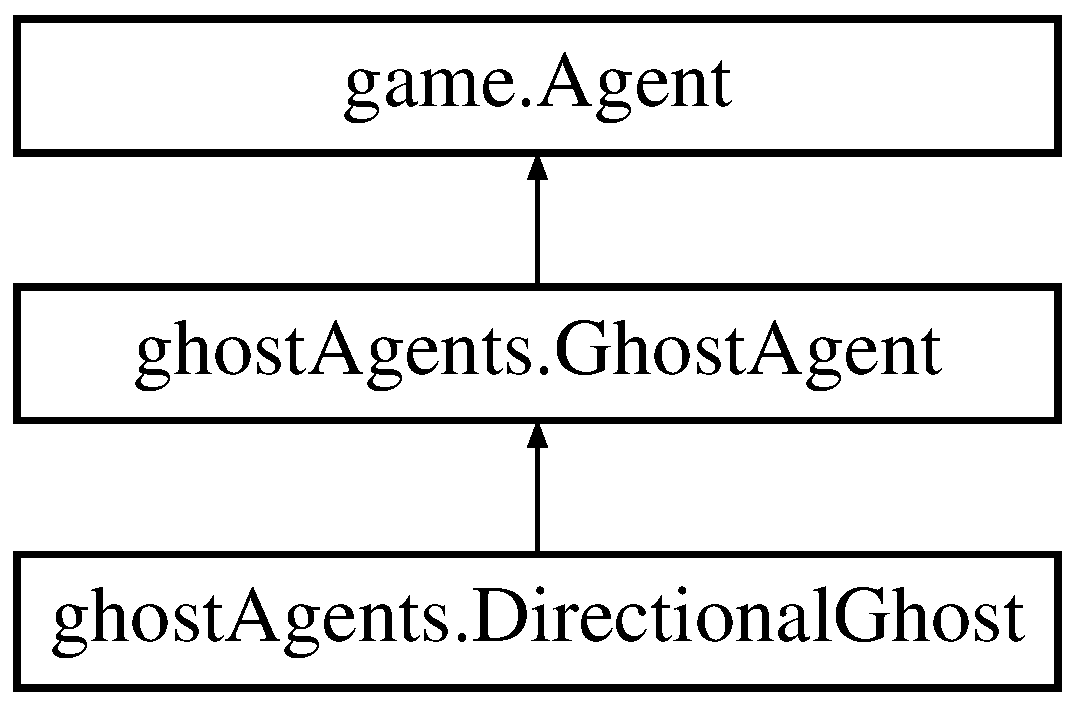
\includegraphics[height=3.000000cm]{classghost_agents_1_1_directional_ghost}
\end{center}
\end{figure}
\subsection*{Public Member Functions}
\begin{DoxyCompactItemize}
\item 
\mbox{\Hypertarget{classghost_agents_1_1_directional_ghost_a84a7ad40273af539193b243bdc779229}\label{classghost_agents_1_1_directional_ghost_a84a7ad40273af539193b243bdc779229}} 
def {\bfseries \+\_\+\+\_\+init\+\_\+\+\_\+} (self, index, prob\+\_\+attack=0.\+8, prob\+\_\+scared\+Flee=0.\+8)
\item 
\mbox{\Hypertarget{classghost_agents_1_1_directional_ghost_a1cb409334e25ac21e3a59e27d781492c}\label{classghost_agents_1_1_directional_ghost_a1cb409334e25ac21e3a59e27d781492c}} 
def {\bfseries get\+Distribution} (self, state)
\end{DoxyCompactItemize}
\subsection*{Public Attributes}
\begin{DoxyCompactItemize}
\item 
\mbox{\Hypertarget{classghost_agents_1_1_directional_ghost_a66b896f308bd62a74b5e9b4894334025}\label{classghost_agents_1_1_directional_ghost_a66b896f308bd62a74b5e9b4894334025}} 
{\bfseries index}
\item 
\mbox{\Hypertarget{classghost_agents_1_1_directional_ghost_a6af983e40d698f5ef02eb6ced4f099cf}\label{classghost_agents_1_1_directional_ghost_a6af983e40d698f5ef02eb6ced4f099cf}} 
{\bfseries prob\+\_\+attack}
\item 
\mbox{\Hypertarget{classghost_agents_1_1_directional_ghost_a69be6e3e8116781a1b24889f5d938c13}\label{classghost_agents_1_1_directional_ghost_a69be6e3e8116781a1b24889f5d938c13}} 
{\bfseries prob\+\_\+scared\+Flee}
\end{DoxyCompactItemize}


The documentation for this class was generated from the following file\+:\begin{DoxyCompactItemize}
\item 
ghost\+Agents.\+py\end{DoxyCompactItemize}

\hypertarget{classgame_1_1_directions}{}\section{game.\+Directions Class Reference}
\label{classgame_1_1_directions}\index{game.\+Directions@{game.\+Directions}}
\subsection*{Static Public Attributes}
\begin{DoxyCompactItemize}
\item 
\mbox{\Hypertarget{classgame_1_1_directions_a1fff6a8a68dbe00f087721d5baceae5c}\label{classgame_1_1_directions_a1fff6a8a68dbe00f087721d5baceae5c}} 
string {\bfseries N\+O\+R\+TH} = \textquotesingle{}North\textquotesingle{}
\item 
\mbox{\Hypertarget{classgame_1_1_directions_ae5858669bbb5df1decffc5607937a2fa}\label{classgame_1_1_directions_ae5858669bbb5df1decffc5607937a2fa}} 
string {\bfseries S\+O\+U\+TH} = \textquotesingle{}South\textquotesingle{}
\item 
\mbox{\Hypertarget{classgame_1_1_directions_ae57293958ef150fea46fcbf5b895972b}\label{classgame_1_1_directions_ae57293958ef150fea46fcbf5b895972b}} 
string {\bfseries E\+A\+ST} = \textquotesingle{}East\textquotesingle{}
\item 
\mbox{\Hypertarget{classgame_1_1_directions_a65ff55da10c03aa93e469ef4d7464994}\label{classgame_1_1_directions_a65ff55da10c03aa93e469ef4d7464994}} 
string {\bfseries W\+E\+ST} = \textquotesingle{}West\textquotesingle{}
\item 
\mbox{\Hypertarget{classgame_1_1_directions_aadd50b4011221fe87cc99c16ecf3c2b2}\label{classgame_1_1_directions_aadd50b4011221fe87cc99c16ecf3c2b2}} 
string {\bfseries S\+T\+OP} = \textquotesingle{}Stop\textquotesingle{}
\item 
dictionary {\bfseries L\+E\+FT}
\item 
\mbox{\Hypertarget{classgame_1_1_directions_a2e9fca42b9c0e302aaf712fe3d3ad5be}\label{classgame_1_1_directions_a2e9fca42b9c0e302aaf712fe3d3ad5be}} 
{\bfseries R\+I\+G\+HT} = dict(\mbox{[}(y,x) for x, y in list(L\+E\+F\+T.\+items())\mbox{]})
\item 
dictionary {\bfseries R\+E\+V\+E\+R\+SE}
\end{DoxyCompactItemize}


\subsection{Member Data Documentation}
\mbox{\Hypertarget{classgame_1_1_directions_a862c07c3211023e93b5eadfecabe1957}\label{classgame_1_1_directions_a862c07c3211023e93b5eadfecabe1957}} 
\index{game\+::\+Directions@{game\+::\+Directions}!L\+E\+FT@{L\+E\+FT}}
\index{L\+E\+FT@{L\+E\+FT}!game\+::\+Directions@{game\+::\+Directions}}
\subsubsection{\texorpdfstring{L\+E\+FT}{LEFT}}
{\footnotesize\ttfamily dictionary game.\+Directions.\+L\+E\+FT\hspace{0.3cm}{\ttfamily [static]}}

{\bfseries Initial value\+:}
\begin{DoxyCode}
=        \{NORTH: WEST,
                 SOUTH: EAST,
                 EAST:  NORTH,
                 WEST:  SOUTH,
                 STOP:  STOP\}
\end{DoxyCode}
\mbox{\Hypertarget{classgame_1_1_directions_ad48d0bb573f126a729c998b505812807}\label{classgame_1_1_directions_ad48d0bb573f126a729c998b505812807}} 
\index{game\+::\+Directions@{game\+::\+Directions}!R\+E\+V\+E\+R\+SE@{R\+E\+V\+E\+R\+SE}}
\index{R\+E\+V\+E\+R\+SE@{R\+E\+V\+E\+R\+SE}!game\+::\+Directions@{game\+::\+Directions}}
\subsubsection{\texorpdfstring{R\+E\+V\+E\+R\+SE}{REVERSE}}
{\footnotesize\ttfamily dictionary game.\+Directions.\+R\+E\+V\+E\+R\+SE\hspace{0.3cm}{\ttfamily [static]}}

{\bfseries Initial value\+:}
\begin{DoxyCode}
=  \{NORTH: SOUTH,
             SOUTH: NORTH,
             EAST: WEST,
             WEST: EAST,
             STOP: STOP\}
\end{DoxyCode}


The documentation for this class was generated from the following file\+:\begin{DoxyCompactItemize}
\item 
game.\+py\end{DoxyCompactItemize}

\hypertarget{classeightpuzzle_1_1_eight_puzzle_search_problem}{}\section{eightpuzzle.\+Eight\+Puzzle\+Search\+Problem Class Reference}
\label{classeightpuzzle_1_1_eight_puzzle_search_problem}\index{eightpuzzle.\+Eight\+Puzzle\+Search\+Problem@{eightpuzzle.\+Eight\+Puzzle\+Search\+Problem}}
Inheritance diagram for eightpuzzle.\+Eight\+Puzzle\+Search\+Problem\+:\begin{figure}[H]
\begin{center}
\leavevmode
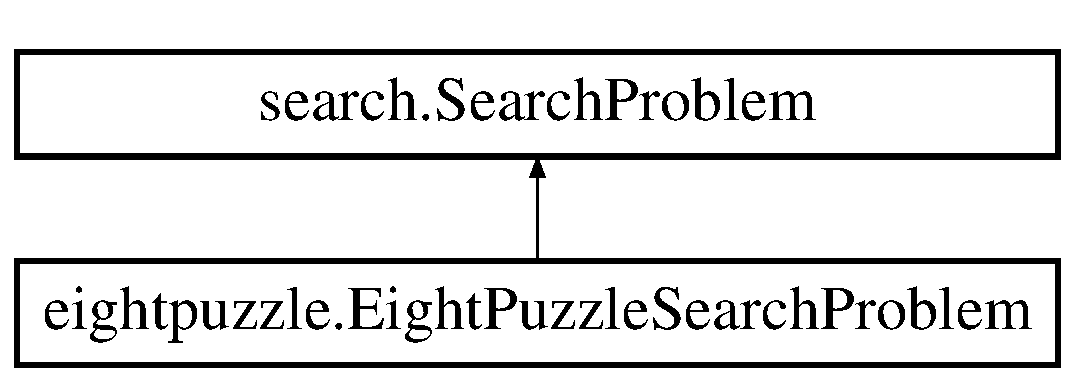
\includegraphics[height=2.000000cm]{classeightpuzzle_1_1_eight_puzzle_search_problem}
\end{center}
\end{figure}
\subsection*{Public Member Functions}
\begin{DoxyCompactItemize}
\item 
\mbox{\Hypertarget{classeightpuzzle_1_1_eight_puzzle_search_problem_ae8bb59255259b3571f333e448c1ec097}\label{classeightpuzzle_1_1_eight_puzzle_search_problem_ae8bb59255259b3571f333e448c1ec097}} 
def {\bfseries \+\_\+\+\_\+init\+\_\+\+\_\+} (self, puzzle)
\item 
\mbox{\Hypertarget{classeightpuzzle_1_1_eight_puzzle_search_problem_ac291c65dbf03a5c060b5a34c04e922bc}\label{classeightpuzzle_1_1_eight_puzzle_search_problem_ac291c65dbf03a5c060b5a34c04e922bc}} 
def {\bfseries get\+Start\+State} (self)
\item 
\mbox{\Hypertarget{classeightpuzzle_1_1_eight_puzzle_search_problem_a9679f43fd8503aaf20c101ecc66bd2ba}\label{classeightpuzzle_1_1_eight_puzzle_search_problem_a9679f43fd8503aaf20c101ecc66bd2ba}} 
def {\bfseries is\+Goal\+State} (self, state)
\item 
def \hyperlink{classeightpuzzle_1_1_eight_puzzle_search_problem_ac33cc3422f9a66bc0270ce43a79cf7c9}{get\+Successors} (self, state)
\item 
def \hyperlink{classeightpuzzle_1_1_eight_puzzle_search_problem_ac2a259f6cf252108fb8560345f788614}{get\+Cost\+Of\+Actions} (self, actions)
\end{DoxyCompactItemize}
\subsection*{Public Attributes}
\begin{DoxyCompactItemize}
\item 
\mbox{\Hypertarget{classeightpuzzle_1_1_eight_puzzle_search_problem_ae16bdf2f41d837d6a79de5528d0b39b4}\label{classeightpuzzle_1_1_eight_puzzle_search_problem_ae16bdf2f41d837d6a79de5528d0b39b4}} 
{\bfseries puzzle}
\end{DoxyCompactItemize}


\subsection{Detailed Description}
\begin{DoxyVerb}  Implementation of a SearchProblem for the  Eight Puzzle domain

  Each state is represented by an instance of an eightPuzzle.
\end{DoxyVerb}
 

\subsection{Member Function Documentation}
\mbox{\Hypertarget{classeightpuzzle_1_1_eight_puzzle_search_problem_ac2a259f6cf252108fb8560345f788614}\label{classeightpuzzle_1_1_eight_puzzle_search_problem_ac2a259f6cf252108fb8560345f788614}} 
\index{eightpuzzle\+::\+Eight\+Puzzle\+Search\+Problem@{eightpuzzle\+::\+Eight\+Puzzle\+Search\+Problem}!get\+Cost\+Of\+Actions@{get\+Cost\+Of\+Actions}}
\index{get\+Cost\+Of\+Actions@{get\+Cost\+Of\+Actions}!eightpuzzle\+::\+Eight\+Puzzle\+Search\+Problem@{eightpuzzle\+::\+Eight\+Puzzle\+Search\+Problem}}
\subsubsection{\texorpdfstring{get\+Cost\+Of\+Actions()}{getCostOfActions()}}
{\footnotesize\ttfamily def eightpuzzle.\+Eight\+Puzzle\+Search\+Problem.\+get\+Cost\+Of\+Actions (\begin{DoxyParamCaption}\item[{}]{self,  }\item[{}]{actions }\end{DoxyParamCaption})}

\begin{DoxyVerb} actions: A list of actions to take

This method returns the total cost of a particular sequence of actions.  The sequence must
be composed of legal moves
\end{DoxyVerb}
 \mbox{\Hypertarget{classeightpuzzle_1_1_eight_puzzle_search_problem_ac33cc3422f9a66bc0270ce43a79cf7c9}\label{classeightpuzzle_1_1_eight_puzzle_search_problem_ac33cc3422f9a66bc0270ce43a79cf7c9}} 
\index{eightpuzzle\+::\+Eight\+Puzzle\+Search\+Problem@{eightpuzzle\+::\+Eight\+Puzzle\+Search\+Problem}!get\+Successors@{get\+Successors}}
\index{get\+Successors@{get\+Successors}!eightpuzzle\+::\+Eight\+Puzzle\+Search\+Problem@{eightpuzzle\+::\+Eight\+Puzzle\+Search\+Problem}}
\subsubsection{\texorpdfstring{get\+Successors()}{getSuccessors()}}
{\footnotesize\ttfamily def eightpuzzle.\+Eight\+Puzzle\+Search\+Problem.\+get\+Successors (\begin{DoxyParamCaption}\item[{}]{self,  }\item[{}]{state }\end{DoxyParamCaption})}

\begin{DoxyVerb}  Returns list of (successor, action, stepCost) pairs where
  each succesor is either left, right, up, or down
  from the original state and the cost is 1.0 for each
\end{DoxyVerb}
 

The documentation for this class was generated from the following file\+:\begin{DoxyCompactItemize}
\item 
eightpuzzle.\+py\end{DoxyCompactItemize}

\hypertarget{classeightpuzzle_1_1_eight_puzzle_state}{}\section{eightpuzzle.\+Eight\+Puzzle\+State Class Reference}
\label{classeightpuzzle_1_1_eight_puzzle_state}\index{eightpuzzle.\+Eight\+Puzzle\+State@{eightpuzzle.\+Eight\+Puzzle\+State}}
\subsection*{Public Member Functions}
\begin{DoxyCompactItemize}
\item 
def \hyperlink{classeightpuzzle_1_1_eight_puzzle_state_a22373dfcbc8746448ef4eb2835694da4}{\+\_\+\+\_\+init\+\_\+\+\_\+} (self, numbers)
\item 
def \hyperlink{classeightpuzzle_1_1_eight_puzzle_state_a39205d164e781dcce7851fc757bf6299}{is\+Goal} (self)
\item 
def \hyperlink{classeightpuzzle_1_1_eight_puzzle_state_a84b1f014353df672abaa38767b775728}{legal\+Moves} (self)
\item 
def \hyperlink{classeightpuzzle_1_1_eight_puzzle_state_a00709c78e645608fffc3fd44d9941519}{result} (self, move)
\item 
def \hyperlink{classeightpuzzle_1_1_eight_puzzle_state_a1a6cd623a0dbba6f268db9a46e3e15e0}{\+\_\+\+\_\+eq\+\_\+\+\_\+} (self, other)
\item 
\mbox{\Hypertarget{classeightpuzzle_1_1_eight_puzzle_state_af31f474616ddc6e1aab9272e0bd13a65}\label{classeightpuzzle_1_1_eight_puzzle_state_af31f474616ddc6e1aab9272e0bd13a65}} 
def {\bfseries \+\_\+\+\_\+hash\+\_\+\+\_\+} (self)
\item 
\mbox{\Hypertarget{classeightpuzzle_1_1_eight_puzzle_state_ab76b60f496605098988ef3267e93aae1}\label{classeightpuzzle_1_1_eight_puzzle_state_ab76b60f496605098988ef3267e93aae1}} 
def {\bfseries \+\_\+\+\_\+str\+\_\+\+\_\+} (self)
\end{DoxyCompactItemize}
\subsection*{Public Attributes}
\begin{DoxyCompactItemize}
\item 
\mbox{\Hypertarget{classeightpuzzle_1_1_eight_puzzle_state_a3508c785ca25b87681f10b32baa6f53d}\label{classeightpuzzle_1_1_eight_puzzle_state_a3508c785ca25b87681f10b32baa6f53d}} 
{\bfseries cells}
\item 
\mbox{\Hypertarget{classeightpuzzle_1_1_eight_puzzle_state_a515568111d27afb30819275eff1f2ccb}\label{classeightpuzzle_1_1_eight_puzzle_state_a515568111d27afb30819275eff1f2ccb}} 
{\bfseries blank\+Location}
\end{DoxyCompactItemize}


\subsection{Detailed Description}
\begin{DoxyVerb}The Eight Puzzle is described in the course textbook on
page 64.

This class defines the mechanics of the puzzle itself.  The
task of recasting this puzzle as a search problem is left to
the EightPuzzleSearchProblem class.
\end{DoxyVerb}
 

\subsection{Constructor \& Destructor Documentation}
\mbox{\Hypertarget{classeightpuzzle_1_1_eight_puzzle_state_a22373dfcbc8746448ef4eb2835694da4}\label{classeightpuzzle_1_1_eight_puzzle_state_a22373dfcbc8746448ef4eb2835694da4}} 
\index{eightpuzzle\+::\+Eight\+Puzzle\+State@{eightpuzzle\+::\+Eight\+Puzzle\+State}!\+\_\+\+\_\+init\+\_\+\+\_\+@{\+\_\+\+\_\+init\+\_\+\+\_\+}}
\index{\+\_\+\+\_\+init\+\_\+\+\_\+@{\+\_\+\+\_\+init\+\_\+\+\_\+}!eightpuzzle\+::\+Eight\+Puzzle\+State@{eightpuzzle\+::\+Eight\+Puzzle\+State}}
\subsubsection{\texorpdfstring{\+\_\+\+\_\+init\+\_\+\+\_\+()}{\_\_init\_\_()}}
{\footnotesize\ttfamily def eightpuzzle.\+Eight\+Puzzle\+State.\+\_\+\+\_\+init\+\_\+\+\_\+ (\begin{DoxyParamCaption}\item[{}]{self,  }\item[{}]{numbers }\end{DoxyParamCaption})}

\begin{DoxyVerb}  Constructs a new eight puzzle from an ordering of numbers.

numbers: a list of integers from 0 to 8 representing an
  instance of the eight puzzle.  0 represents the blank
  space.  Thus, the list

 [1, 0, 2, 3, 4, 5, 6, 7, 8]

  represents the eight puzzle:
 -------------
 | 1 |   | 2 |
 -------------
 | 3 | 4 | 5 |
 -------------
 | 6 | 7 | 8 |
 ------------

The configuration of the puzzle is stored in a 2-dimensional
list (a list of lists) 'cells'.
\end{DoxyVerb}
 

\subsection{Member Function Documentation}
\mbox{\Hypertarget{classeightpuzzle_1_1_eight_puzzle_state_a1a6cd623a0dbba6f268db9a46e3e15e0}\label{classeightpuzzle_1_1_eight_puzzle_state_a1a6cd623a0dbba6f268db9a46e3e15e0}} 
\index{eightpuzzle\+::\+Eight\+Puzzle\+State@{eightpuzzle\+::\+Eight\+Puzzle\+State}!\+\_\+\+\_\+eq\+\_\+\+\_\+@{\+\_\+\+\_\+eq\+\_\+\+\_\+}}
\index{\+\_\+\+\_\+eq\+\_\+\+\_\+@{\+\_\+\+\_\+eq\+\_\+\+\_\+}!eightpuzzle\+::\+Eight\+Puzzle\+State@{eightpuzzle\+::\+Eight\+Puzzle\+State}}
\subsubsection{\texorpdfstring{\+\_\+\+\_\+eq\+\_\+\+\_\+()}{\_\_eq\_\_()}}
{\footnotesize\ttfamily def eightpuzzle.\+Eight\+Puzzle\+State.\+\_\+\+\_\+eq\+\_\+\+\_\+ (\begin{DoxyParamCaption}\item[{}]{self,  }\item[{}]{other }\end{DoxyParamCaption})}

\begin{DoxyVerb} Overloads '==' such that two eightPuzzles with the same configuration
  are equal.

  >>> EightPuzzleState([0, 1, 2, 3, 4, 5, 6, 7, 8]) == \
   EightPuzzleState([1, 0, 2, 3, 4, 5, 6, 7, 8]).result('left')
  True
\end{DoxyVerb}
 \mbox{\Hypertarget{classeightpuzzle_1_1_eight_puzzle_state_a39205d164e781dcce7851fc757bf6299}\label{classeightpuzzle_1_1_eight_puzzle_state_a39205d164e781dcce7851fc757bf6299}} 
\index{eightpuzzle\+::\+Eight\+Puzzle\+State@{eightpuzzle\+::\+Eight\+Puzzle\+State}!is\+Goal@{is\+Goal}}
\index{is\+Goal@{is\+Goal}!eightpuzzle\+::\+Eight\+Puzzle\+State@{eightpuzzle\+::\+Eight\+Puzzle\+State}}
\subsubsection{\texorpdfstring{is\+Goal()}{isGoal()}}
{\footnotesize\ttfamily def eightpuzzle.\+Eight\+Puzzle\+State.\+is\+Goal (\begin{DoxyParamCaption}\item[{}]{self }\end{DoxyParamCaption})}

\begin{DoxyVerb}  Checks to see if the puzzle is in its goal state.

 -------------
 |   | 1 | 2 |
 -------------
 | 3 | 4 | 5 |
 -------------
 | 6 | 7 | 8 |
 -------------

>>> EightPuzzleState([0, 1, 2, 3, 4, 5, 6, 7, 8]).isGoal()
True

>>> EightPuzzleState([1, 0, 2, 3, 4, 5, 6, 7, 8]).isGoal()
False
\end{DoxyVerb}
 \mbox{\Hypertarget{classeightpuzzle_1_1_eight_puzzle_state_a84b1f014353df672abaa38767b775728}\label{classeightpuzzle_1_1_eight_puzzle_state_a84b1f014353df672abaa38767b775728}} 
\index{eightpuzzle\+::\+Eight\+Puzzle\+State@{eightpuzzle\+::\+Eight\+Puzzle\+State}!legal\+Moves@{legal\+Moves}}
\index{legal\+Moves@{legal\+Moves}!eightpuzzle\+::\+Eight\+Puzzle\+State@{eightpuzzle\+::\+Eight\+Puzzle\+State}}
\subsubsection{\texorpdfstring{legal\+Moves()}{legalMoves()}}
{\footnotesize\ttfamily def eightpuzzle.\+Eight\+Puzzle\+State.\+legal\+Moves (\begin{DoxyParamCaption}\item[{}]{self }\end{DoxyParamCaption})}

\begin{DoxyVerb}  Returns a list of legal moves from the current state.

Moves consist of moving the blank space up, down, left or right.
These are encoded as 'up', 'down', 'left' and 'right' respectively.

>>> EightPuzzleState([0, 1, 2, 3, 4, 5, 6, 7, 8]).legalMoves()
['down', 'right']
\end{DoxyVerb}
 \mbox{\Hypertarget{classeightpuzzle_1_1_eight_puzzle_state_a00709c78e645608fffc3fd44d9941519}\label{classeightpuzzle_1_1_eight_puzzle_state_a00709c78e645608fffc3fd44d9941519}} 
\index{eightpuzzle\+::\+Eight\+Puzzle\+State@{eightpuzzle\+::\+Eight\+Puzzle\+State}!result@{result}}
\index{result@{result}!eightpuzzle\+::\+Eight\+Puzzle\+State@{eightpuzzle\+::\+Eight\+Puzzle\+State}}
\subsubsection{\texorpdfstring{result()}{result()}}
{\footnotesize\ttfamily def eightpuzzle.\+Eight\+Puzzle\+State.\+result (\begin{DoxyParamCaption}\item[{}]{self,  }\item[{}]{move }\end{DoxyParamCaption})}

\begin{DoxyVerb}  Returns a new eightPuzzle with the current state and blankLocation
updated based on the provided move.

The move should be a string drawn from a list returned by legalMoves.
Illegal moves will raise an exception, which may be an array bounds
exception.

NOTE: This function *does not* change the current object.  Instead,
it returns a new object.
\end{DoxyVerb}
 

The documentation for this class was generated from the following file\+:\begin{DoxyCompactItemize}
\item 
eightpuzzle.\+py\end{DoxyCompactItemize}

\hypertarget{classgraphics_display_1_1_first_person_pacman_graphics}{}\section{graphics\+Display.\+First\+Person\+Pacman\+Graphics Class Reference}
\label{classgraphics_display_1_1_first_person_pacman_graphics}\index{graphics\+Display.\+First\+Person\+Pacman\+Graphics@{graphics\+Display.\+First\+Person\+Pacman\+Graphics}}
Inheritance diagram for graphics\+Display.\+First\+Person\+Pacman\+Graphics\+:\begin{figure}[H]
\begin{center}
\leavevmode
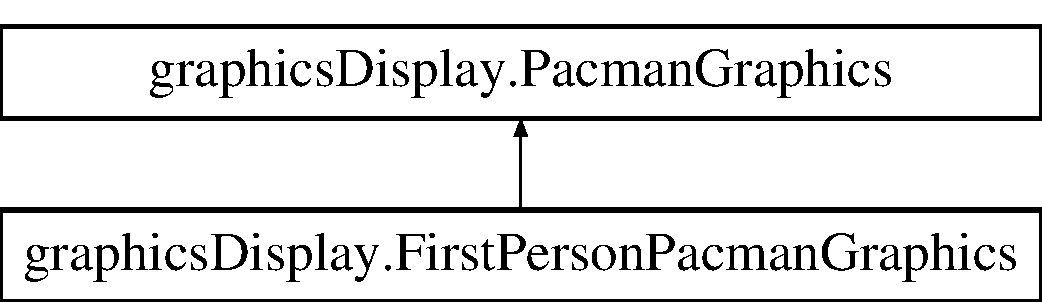
\includegraphics[height=2.000000cm]{classgraphics_display_1_1_first_person_pacman_graphics}
\end{center}
\end{figure}
\subsection*{Public Member Functions}
\begin{DoxyCompactItemize}
\item 
\mbox{\Hypertarget{classgraphics_display_1_1_first_person_pacman_graphics_a9a4254cdca8646924056b36442d89ee4}\label{classgraphics_display_1_1_first_person_pacman_graphics_a9a4254cdca8646924056b36442d89ee4}} 
def {\bfseries \+\_\+\+\_\+init\+\_\+\+\_\+} (self, zoom=1.\+0, show\+Ghosts=True, capture=False, frame\+Time=0)
\item 
\mbox{\Hypertarget{classgraphics_display_1_1_first_person_pacman_graphics_a43779a7ad6e7ee48c7169b4b5312ccd1}\label{classgraphics_display_1_1_first_person_pacman_graphics_a43779a7ad6e7ee48c7169b4b5312ccd1}} 
def {\bfseries initialize} (self, state, is\+Blue=False)
\item 
\mbox{\Hypertarget{classgraphics_display_1_1_first_person_pacman_graphics_a6996651f68d57f2e405dbcc57e8d29ac}\label{classgraphics_display_1_1_first_person_pacman_graphics_a6996651f68d57f2e405dbcc57e8d29ac}} 
def {\bfseries look\+Ahead} (self, config, state)
\item 
\mbox{\Hypertarget{classgraphics_display_1_1_first_person_pacman_graphics_a7c603b3281c4d2d0ac672e6344e29798}\label{classgraphics_display_1_1_first_person_pacman_graphics_a7c603b3281c4d2d0ac672e6344e29798}} 
def {\bfseries get\+Ghost\+Color} (self, ghost, ghost\+Index)
\item 
\mbox{\Hypertarget{classgraphics_display_1_1_first_person_pacman_graphics_aa5628ea291a7f5b2650f27cd147711e5}\label{classgraphics_display_1_1_first_person_pacman_graphics_aa5628ea291a7f5b2650f27cd147711e5}} 
def {\bfseries get\+Position} (self, ghost\+State)
\end{DoxyCompactItemize}
\subsection*{Public Attributes}
\begin{DoxyCompactItemize}
\item 
\mbox{\Hypertarget{classgraphics_display_1_1_first_person_pacman_graphics_aae1ccb9db807d50f65415a19a48485a9}\label{classgraphics_display_1_1_first_person_pacman_graphics_aae1ccb9db807d50f65415a19a48485a9}} 
{\bfseries show\+Ghosts}
\item 
\mbox{\Hypertarget{classgraphics_display_1_1_first_person_pacman_graphics_af14d89fcadf1b96c2b288b03c173cd49}\label{classgraphics_display_1_1_first_person_pacman_graphics_af14d89fcadf1b96c2b288b03c173cd49}} 
{\bfseries capture}
\item 
\mbox{\Hypertarget{classgraphics_display_1_1_first_person_pacman_graphics_ae032aba81cef88b005ad440771120fb8}\label{classgraphics_display_1_1_first_person_pacman_graphics_ae032aba81cef88b005ad440771120fb8}} 
{\bfseries is\+Blue}
\item 
\mbox{\Hypertarget{classgraphics_display_1_1_first_person_pacman_graphics_a3b7983e2c15de390851a03c501099131}\label{classgraphics_display_1_1_first_person_pacman_graphics_a3b7983e2c15de390851a03c501099131}} 
{\bfseries layout}
\item 
\mbox{\Hypertarget{classgraphics_display_1_1_first_person_pacman_graphics_a39c1689911d46d847ceef6c4aa1b4500}\label{classgraphics_display_1_1_first_person_pacman_graphics_a39c1689911d46d847ceef6c4aa1b4500}} 
{\bfseries distribution\+Images}
\item 
\mbox{\Hypertarget{classgraphics_display_1_1_first_person_pacman_graphics_a6a9abfa36d0d270894d33a1e17b1e148}\label{classgraphics_display_1_1_first_person_pacman_graphics_a6a9abfa36d0d270894d33a1e17b1e148}} 
{\bfseries previous\+State}
\end{DoxyCompactItemize}


The documentation for this class was generated from the following file\+:\begin{DoxyCompactItemize}
\item 
graphics\+Display.\+py\end{DoxyCompactItemize}

\hypertarget{classsearch_agents_1_1_food_search_problem}{}\section{search\+Agents.\+Food\+Search\+Problem Class Reference}
\label{classsearch_agents_1_1_food_search_problem}\index{search\+Agents.\+Food\+Search\+Problem@{search\+Agents.\+Food\+Search\+Problem}}
\subsection*{Public Member Functions}
\begin{DoxyCompactItemize}
\item 
\mbox{\Hypertarget{classsearch_agents_1_1_food_search_problem_aceb4d4d29de50f107fa13e25e7d0be74}\label{classsearch_agents_1_1_food_search_problem_aceb4d4d29de50f107fa13e25e7d0be74}} 
def {\bfseries \+\_\+\+\_\+init\+\_\+\+\_\+} (self, starting\+Game\+State)
\item 
\mbox{\Hypertarget{classsearch_agents_1_1_food_search_problem_af3ef21c5f2c240580642904a471d7073}\label{classsearch_agents_1_1_food_search_problem_af3ef21c5f2c240580642904a471d7073}} 
def {\bfseries get\+Start\+State} (self)
\item 
\mbox{\Hypertarget{classsearch_agents_1_1_food_search_problem_abc299d7e9ab66fa115f43baa0fdd7fbf}\label{classsearch_agents_1_1_food_search_problem_abc299d7e9ab66fa115f43baa0fdd7fbf}} 
def {\bfseries is\+Goal\+State} (self, state)
\item 
\mbox{\Hypertarget{classsearch_agents_1_1_food_search_problem_aa892375d4b57691f981999a870c6734d}\label{classsearch_agents_1_1_food_search_problem_aa892375d4b57691f981999a870c6734d}} 
def {\bfseries get\+Successors} (self, state)
\item 
def \hyperlink{classsearch_agents_1_1_food_search_problem_a77b77a7182bb81a22a67f0b48170da2c}{get\+Cost\+Of\+Actions} (self, actions)
\end{DoxyCompactItemize}
\subsection*{Public Attributes}
\begin{DoxyCompactItemize}
\item 
\mbox{\Hypertarget{classsearch_agents_1_1_food_search_problem_a4ef87b14faf538073a2b15cf7c3d425d}\label{classsearch_agents_1_1_food_search_problem_a4ef87b14faf538073a2b15cf7c3d425d}} 
{\bfseries start}
\item 
\mbox{\Hypertarget{classsearch_agents_1_1_food_search_problem_a453ebb7aa98704cf8ccac7dc98157494}\label{classsearch_agents_1_1_food_search_problem_a453ebb7aa98704cf8ccac7dc98157494}} 
{\bfseries walls}
\item 
\mbox{\Hypertarget{classsearch_agents_1_1_food_search_problem_a53eb097b181626e977c8fe5a337c1a1a}\label{classsearch_agents_1_1_food_search_problem_a53eb097b181626e977c8fe5a337c1a1a}} 
{\bfseries starting\+Game\+State}
\item 
\mbox{\Hypertarget{classsearch_agents_1_1_food_search_problem_a5ed921e24b8daf256d6738415f1e22c1}\label{classsearch_agents_1_1_food_search_problem_a5ed921e24b8daf256d6738415f1e22c1}} 
{\bfseries heuristic\+Info}
\end{DoxyCompactItemize}


\subsection{Detailed Description}
\begin{DoxyVerb}A search problem associated with finding the a path that collects all of the
food (dots) in a Pacman game.

A search state in this problem is a tuple ( pacmanPosition, foodGrid ) where
  pacmanPosition: a tuple (x,y) of integers specifying Pacman's position
  foodGrid:       a Grid (see game.py) of either True or False, specifying remaining food
\end{DoxyVerb}
 

\subsection{Member Function Documentation}
\mbox{\Hypertarget{classsearch_agents_1_1_food_search_problem_a77b77a7182bb81a22a67f0b48170da2c}\label{classsearch_agents_1_1_food_search_problem_a77b77a7182bb81a22a67f0b48170da2c}} 
\index{search\+Agents\+::\+Food\+Search\+Problem@{search\+Agents\+::\+Food\+Search\+Problem}!get\+Cost\+Of\+Actions@{get\+Cost\+Of\+Actions}}
\index{get\+Cost\+Of\+Actions@{get\+Cost\+Of\+Actions}!search\+Agents\+::\+Food\+Search\+Problem@{search\+Agents\+::\+Food\+Search\+Problem}}
\subsubsection{\texorpdfstring{get\+Cost\+Of\+Actions()}{getCostOfActions()}}
{\footnotesize\ttfamily def search\+Agents.\+Food\+Search\+Problem.\+get\+Cost\+Of\+Actions (\begin{DoxyParamCaption}\item[{}]{self,  }\item[{}]{actions }\end{DoxyParamCaption})}

\begin{DoxyVerb}Returns the cost of a particular sequence of actions.  If those actions
include an illegal move, return 999999\end{DoxyVerb}
 

The documentation for this class was generated from the following file\+:\begin{DoxyCompactItemize}
\item 
search\+Agents.\+py\end{DoxyCompactItemize}

\hypertarget{classgame_1_1_game}{}\section{game.\+Game Class Reference}
\label{classgame_1_1_game}\index{game.\+Game@{game.\+Game}}
\subsection*{Public Member Functions}
\begin{DoxyCompactItemize}
\item 
\mbox{\Hypertarget{classgame_1_1_game_a0252ff2844570b8cdb4d8cc2773e38f3}\label{classgame_1_1_game_a0252ff2844570b8cdb4d8cc2773e38f3}} 
def {\bfseries \+\_\+\+\_\+init\+\_\+\+\_\+} (self, agents, display, rules, starting\+Index=0, mute\+Agents=False, catch\+Exceptions=False)
\item 
\mbox{\Hypertarget{classgame_1_1_game_a612b385764b718342a51541d078513bb}\label{classgame_1_1_game_a612b385764b718342a51541d078513bb}} 
def {\bfseries get\+Progress} (self)
\item 
\mbox{\Hypertarget{classgame_1_1_game_a88817c9dc6f5755f999043cdafddf791}\label{classgame_1_1_game_a88817c9dc6f5755f999043cdafddf791}} 
def {\bfseries mute} (self)
\item 
\mbox{\Hypertarget{classgame_1_1_game_a48c3a76f1dc82f1630ee91021cd0db93}\label{classgame_1_1_game_a48c3a76f1dc82f1630ee91021cd0db93}} 
def {\bfseries unmute} (self)
\item 
def \hyperlink{classgame_1_1_game_a5ac60e090ecb22edd8fe33073b45866e}{run} (self)
\end{DoxyCompactItemize}
\subsection*{Public Attributes}
\begin{DoxyCompactItemize}
\item 
\mbox{\Hypertarget{classgame_1_1_game_a3a7bae150ed81271fd683784092b4ef5}\label{classgame_1_1_game_a3a7bae150ed81271fd683784092b4ef5}} 
{\bfseries agent\+Crashed}
\item 
\mbox{\Hypertarget{classgame_1_1_game_a63d26aa71e10bbe4cf44e3e9cb67f353}\label{classgame_1_1_game_a63d26aa71e10bbe4cf44e3e9cb67f353}} 
{\bfseries agents}
\item 
\mbox{\Hypertarget{classgame_1_1_game_a287336b84d466cdb9adca9b189120be9}\label{classgame_1_1_game_a287336b84d466cdb9adca9b189120be9}} 
{\bfseries display}
\item 
\mbox{\Hypertarget{classgame_1_1_game_abf21adb2ae4967476b66346e99e16584}\label{classgame_1_1_game_abf21adb2ae4967476b66346e99e16584}} 
{\bfseries rules}
\item 
\mbox{\Hypertarget{classgame_1_1_game_a75b69405729c4d993b34bf02c4460b91}\label{classgame_1_1_game_a75b69405729c4d993b34bf02c4460b91}} 
{\bfseries starting\+Index}
\item 
\mbox{\Hypertarget{classgame_1_1_game_a8387804bf60984f336a477be8b405ec1}\label{classgame_1_1_game_a8387804bf60984f336a477be8b405ec1}} 
{\bfseries game\+Over}
\item 
\mbox{\Hypertarget{classgame_1_1_game_ad8a2998d104cca6ef043f417948955a9}\label{classgame_1_1_game_ad8a2998d104cca6ef043f417948955a9}} 
{\bfseries mute\+Agents}
\item 
\mbox{\Hypertarget{classgame_1_1_game_ab5a73b31df08fac2afd3f72aed7148b0}\label{classgame_1_1_game_ab5a73b31df08fac2afd3f72aed7148b0}} 
{\bfseries catch\+Exceptions}
\item 
\mbox{\Hypertarget{classgame_1_1_game_a74cd84c26784c541ca2ebeaa4b897a13}\label{classgame_1_1_game_a74cd84c26784c541ca2ebeaa4b897a13}} 
{\bfseries move\+History}
\item 
\mbox{\Hypertarget{classgame_1_1_game_af2a24dc23d93f7f4021498016d0116f0}\label{classgame_1_1_game_af2a24dc23d93f7f4021498016d0116f0}} 
{\bfseries total\+Agent\+Times}
\item 
\mbox{\Hypertarget{classgame_1_1_game_a39cd4c1d2fc487f19a3628d1361d6519}\label{classgame_1_1_game_a39cd4c1d2fc487f19a3628d1361d6519}} 
{\bfseries total\+Agent\+Time\+Warnings}
\item 
\hyperlink{classgame_1_1_game_a269239dbb1e058565244d278b9ba460f}{agent\+Timeout}
\begin{DoxyCompactList}\small\item\em self.\+display.\+initialize(self.\+state.\+make\+Observation(1).data) inform learning agents of the game start \end{DoxyCompactList}\item 
\mbox{\Hypertarget{classgame_1_1_game_a3951c9397f2f303a0724b35622d86b9d}\label{classgame_1_1_game_a3951c9397f2f303a0724b35622d86b9d}} 
{\bfseries num\+Moves}
\item 
\mbox{\Hypertarget{classgame_1_1_game_a3467c8e943cb5c048b3b45bc9b563311}\label{classgame_1_1_game_a3467c8e943cb5c048b3b45bc9b563311}} 
{\bfseries state}
\end{DoxyCompactItemize}
\subsection*{Static Public Attributes}
\begin{DoxyCompactItemize}
\item 
\mbox{\Hypertarget{classgame_1_1_game_a89eff163f532c2e5c8c85f996b4cf936}\label{classgame_1_1_game_a89eff163f532c2e5c8c85f996b4cf936}} 
{\bfseries O\+L\+D\+\_\+\+S\+T\+D\+O\+UT} = None
\item 
\mbox{\Hypertarget{classgame_1_1_game_aaacc3bad55fb2cd0f91acfff08397f9f}\label{classgame_1_1_game_aaacc3bad55fb2cd0f91acfff08397f9f}} 
{\bfseries O\+L\+D\+\_\+\+S\+T\+D\+E\+RR} = None
\end{DoxyCompactItemize}


\subsection{Detailed Description}
\begin{DoxyVerb}The Game manages the control flow, soliciting actions from agents.
\end{DoxyVerb}
 

\subsection{Member Function Documentation}
\mbox{\Hypertarget{classgame_1_1_game_a5ac60e090ecb22edd8fe33073b45866e}\label{classgame_1_1_game_a5ac60e090ecb22edd8fe33073b45866e}} 
\index{game\+::\+Game@{game\+::\+Game}!run@{run}}
\index{run@{run}!game\+::\+Game@{game\+::\+Game}}
\subsubsection{\texorpdfstring{run()}{run()}}
{\footnotesize\ttfamily def game.\+Game.\+run (\begin{DoxyParamCaption}\item[{}]{self }\end{DoxyParamCaption})}

\begin{DoxyVerb}Main control loop for game play.
\end{DoxyVerb}
 

\subsection{Member Data Documentation}
\mbox{\Hypertarget{classgame_1_1_game_a269239dbb1e058565244d278b9ba460f}\label{classgame_1_1_game_a269239dbb1e058565244d278b9ba460f}} 
\index{game\+::\+Game@{game\+::\+Game}!agent\+Timeout@{agent\+Timeout}}
\index{agent\+Timeout@{agent\+Timeout}!game\+::\+Game@{game\+::\+Game}}
\subsubsection{\texorpdfstring{agent\+Timeout}{agentTimeout}}
{\footnotesize\ttfamily game.\+Game.\+agent\+Timeout}



self.\+display.\+initialize(self.\+state.\+make\+Observation(1).data) inform learning agents of the game start 

T\+O\+DO\+: could this exceed the total time. 

The documentation for this class was generated from the following file\+:\begin{DoxyCompactItemize}
\item 
game.\+py\end{DoxyCompactItemize}

\hypertarget{classpacman_1_1_game_state}{}\section{pacman.\+Game\+State Class Reference}
\label{classpacman_1_1_game_state}\index{pacman.\+Game\+State@{pacman.\+Game\+State}}


Y\+O\+UR I\+N\+T\+E\+R\+F\+A\+CE TO T\+HE P\+A\+C\+M\+AN W\+O\+R\+LD\+: A \hyperlink{classpacman_1_1_game_state}{Game\+State} \#.  


\subsection*{Public Member Functions}
\begin{DoxyCompactItemize}
\item 
def \hyperlink{classpacman_1_1_game_state_a052ecff567f806c589fa08f21c8d3b15}{get\+Legal\+Actions} (self, agent\+Index=0)
\begin{DoxyCompactList}\small\item\em Accessor methods\+: use these to access state data \#. \end{DoxyCompactList}\item 
def \hyperlink{classpacman_1_1_game_state_a1c66e94fa4b64bce020b711bfefd4d81}{generate\+Successor} (self, agent\+Index, action)
\item 
\mbox{\Hypertarget{classpacman_1_1_game_state_ad3301e604605140a6097fc89dc044eec}\label{classpacman_1_1_game_state_ad3301e604605140a6097fc89dc044eec}} 
def {\bfseries get\+Legal\+Pacman\+Actions} (self)
\item 
def \hyperlink{classpacman_1_1_game_state_a944c5f5ba5f3c356db326602e5734451}{generate\+Pacman\+Successor} (self, action)
\item 
def \hyperlink{classpacman_1_1_game_state_a5e17856afbfa1f0a0fbafcff73878fd8}{get\+Pacman\+State} (self)
\item 
\mbox{\Hypertarget{classpacman_1_1_game_state_a33d07b517901bff5476830815c2fbc15}\label{classpacman_1_1_game_state_a33d07b517901bff5476830815c2fbc15}} 
def {\bfseries get\+Pacman\+Position} (self)
\item 
\mbox{\Hypertarget{classpacman_1_1_game_state_af1cb7ad188ec2f5f2ea8a2ff2a9b9c98}\label{classpacman_1_1_game_state_af1cb7ad188ec2f5f2ea8a2ff2a9b9c98}} 
def {\bfseries get\+Ghost\+States} (self)
\item 
\mbox{\Hypertarget{classpacman_1_1_game_state_a8751dd97bc037d03bfacef57bffbfd83}\label{classpacman_1_1_game_state_a8751dd97bc037d03bfacef57bffbfd83}} 
def {\bfseries get\+Ghost\+State} (self, agent\+Index)
\item 
\mbox{\Hypertarget{classpacman_1_1_game_state_a772374c3d2df51eda98d610baae1db8d}\label{classpacman_1_1_game_state_a772374c3d2df51eda98d610baae1db8d}} 
def {\bfseries get\+Ghost\+Position} (self, agent\+Index)
\item 
\mbox{\Hypertarget{classpacman_1_1_game_state_a4485dbbf65e0f98412a402edbbcb9a9a}\label{classpacman_1_1_game_state_a4485dbbf65e0f98412a402edbbcb9a9a}} 
def {\bfseries get\+Ghost\+Positions} (self)
\item 
\mbox{\Hypertarget{classpacman_1_1_game_state_ad19bd7f4416300f647108c86e5be28f4}\label{classpacman_1_1_game_state_ad19bd7f4416300f647108c86e5be28f4}} 
def {\bfseries get\+Num\+Agents} (self)
\item 
\mbox{\Hypertarget{classpacman_1_1_game_state_a7b3dff620b0d5e278f3ce8813607f7f0}\label{classpacman_1_1_game_state_a7b3dff620b0d5e278f3ce8813607f7f0}} 
def {\bfseries get\+Score} (self)
\item 
def \hyperlink{classpacman_1_1_game_state_a1221e5f48a5acae4f1794c352c8549e8}{get\+Capsules} (self)
\item 
\mbox{\Hypertarget{classpacman_1_1_game_state_a8eb83a19a2e8f2fdaa3bfca97b66cd9f}\label{classpacman_1_1_game_state_a8eb83a19a2e8f2fdaa3bfca97b66cd9f}} 
def {\bfseries get\+Num\+Food} (self)
\item 
def \hyperlink{classpacman_1_1_game_state_a532341ee8ed3d7940681bc6d1c489253}{get\+Food} (self)
\item 
def \hyperlink{classpacman_1_1_game_state_a770ccd37a37643829098559de97f4b09}{get\+Walls} (self)
\item 
\mbox{\Hypertarget{classpacman_1_1_game_state_a01276bec7b87eefa3549473689990433}\label{classpacman_1_1_game_state_a01276bec7b87eefa3549473689990433}} 
def {\bfseries has\+Food} (self, x, y)
\item 
\mbox{\Hypertarget{classpacman_1_1_game_state_a5b5f448d085c24a0c87f3d4abbbfa1c9}\label{classpacman_1_1_game_state_a5b5f448d085c24a0c87f3d4abbbfa1c9}} 
def {\bfseries has\+Wall} (self, x, y)
\item 
\mbox{\Hypertarget{classpacman_1_1_game_state_a10b8e79d9e31c753340d9edccf65f971}\label{classpacman_1_1_game_state_a10b8e79d9e31c753340d9edccf65f971}} 
def {\bfseries is\+Lose} (self)
\item 
\mbox{\Hypertarget{classpacman_1_1_game_state_aa06e9b926f57f62892a5815ed45abde1}\label{classpacman_1_1_game_state_aa06e9b926f57f62892a5815ed45abde1}} 
def {\bfseries is\+Win} (self)
\item 
def \hyperlink{classpacman_1_1_game_state_ab9cd0448f581a626b6fa2f05a5331ca1}{\+\_\+\+\_\+init\+\_\+\+\_\+} (self, prev\+State=None)
\begin{DoxyCompactList}\small\item\em \begin{DoxyVerb}        Helper methods:               #
\end{DoxyVerb}
 You shouldn\textquotesingle{}t need to call these directly \# \end{DoxyCompactList}\item 
\mbox{\Hypertarget{classpacman_1_1_game_state_a9444717b02e2809cb1864f540c544350}\label{classpacman_1_1_game_state_a9444717b02e2809cb1864f540c544350}} 
def {\bfseries deep\+Copy} (self)
\item 
def \hyperlink{classpacman_1_1_game_state_a9a4c4fa4c3744ec2cf1ca3afd232d089}{\+\_\+\+\_\+eq\+\_\+\+\_\+} (self, other)
\item 
def \hyperlink{classpacman_1_1_game_state_a51305408cabe92cebb6282e033a07bca}{\+\_\+\+\_\+hash\+\_\+\+\_\+} (self)
\item 
\mbox{\Hypertarget{classpacman_1_1_game_state_afa63b5c06afb29b9a0660d85d8333834}\label{classpacman_1_1_game_state_afa63b5c06afb29b9a0660d85d8333834}} 
def {\bfseries \+\_\+\+\_\+str\+\_\+\+\_\+} (self)
\item 
def \hyperlink{classpacman_1_1_game_state_a4c6d262e61c43f550cc509e584c559f1}{initialize} (self, layout, num\+Ghost\+Agents=1000)
\end{DoxyCompactItemize}
\subsection*{Public Attributes}
\begin{DoxyCompactItemize}
\item 
\mbox{\Hypertarget{classpacman_1_1_game_state_a3588cad7134271ae1b53dc726535368b}\label{classpacman_1_1_game_state_a3588cad7134271ae1b53dc726535368b}} 
{\bfseries data}
\end{DoxyCompactItemize}


\subsection{Detailed Description}
Y\+O\+UR I\+N\+T\+E\+R\+F\+A\+CE TO T\+HE P\+A\+C\+M\+AN W\+O\+R\+LD\+: A \hyperlink{classpacman_1_1_game_state}{Game\+State} \#. 

\begin{DoxyVerb}A GameState specifies the full game state, including the food, capsules,
agent configurations and score changes.

GameStates are used by the Game object to capture the actual state of the game and
can be used by agents to reason about the game.

Much of the information in a GameState is stored in a GameStateData object.  We
strongly suggest that you access that data via the accessor methods below rather
than referring to the GameStateData object directly.

Note that in classic Pacman, Pacman is always agent 0.
\end{DoxyVerb}
 

\subsection{Constructor \& Destructor Documentation}
\mbox{\Hypertarget{classpacman_1_1_game_state_ab9cd0448f581a626b6fa2f05a5331ca1}\label{classpacman_1_1_game_state_ab9cd0448f581a626b6fa2f05a5331ca1}} 
\index{pacman\+::\+Game\+State@{pacman\+::\+Game\+State}!\+\_\+\+\_\+init\+\_\+\+\_\+@{\+\_\+\+\_\+init\+\_\+\+\_\+}}
\index{\+\_\+\+\_\+init\+\_\+\+\_\+@{\+\_\+\+\_\+init\+\_\+\+\_\+}!pacman\+::\+Game\+State@{pacman\+::\+Game\+State}}
\subsubsection{\texorpdfstring{\+\_\+\+\_\+init\+\_\+\+\_\+()}{\_\_init\_\_()}}
{\footnotesize\ttfamily def pacman.\+Game\+State.\+\_\+\+\_\+init\+\_\+\+\_\+ (\begin{DoxyParamCaption}\item[{}]{self,  }\item[{}]{prev\+State = {\ttfamily None} }\end{DoxyParamCaption})}



\begin{DoxyVerb}        Helper methods:               #
\end{DoxyVerb}
 You shouldn\textquotesingle{}t need to call these directly \# 

\begin{DoxyVerb}Generates a new state by copying information from its predecessor.
\end{DoxyVerb}
 

\subsection{Member Function Documentation}
\mbox{\Hypertarget{classpacman_1_1_game_state_a9a4c4fa4c3744ec2cf1ca3afd232d089}\label{classpacman_1_1_game_state_a9a4c4fa4c3744ec2cf1ca3afd232d089}} 
\index{pacman\+::\+Game\+State@{pacman\+::\+Game\+State}!\+\_\+\+\_\+eq\+\_\+\+\_\+@{\+\_\+\+\_\+eq\+\_\+\+\_\+}}
\index{\+\_\+\+\_\+eq\+\_\+\+\_\+@{\+\_\+\+\_\+eq\+\_\+\+\_\+}!pacman\+::\+Game\+State@{pacman\+::\+Game\+State}}
\subsubsection{\texorpdfstring{\+\_\+\+\_\+eq\+\_\+\+\_\+()}{\_\_eq\_\_()}}
{\footnotesize\ttfamily def pacman.\+Game\+State.\+\_\+\+\_\+eq\+\_\+\+\_\+ (\begin{DoxyParamCaption}\item[{}]{self,  }\item[{}]{other }\end{DoxyParamCaption})}

\begin{DoxyVerb}Allows two states to be compared.
\end{DoxyVerb}
 \mbox{\Hypertarget{classpacman_1_1_game_state_a51305408cabe92cebb6282e033a07bca}\label{classpacman_1_1_game_state_a51305408cabe92cebb6282e033a07bca}} 
\index{pacman\+::\+Game\+State@{pacman\+::\+Game\+State}!\+\_\+\+\_\+hash\+\_\+\+\_\+@{\+\_\+\+\_\+hash\+\_\+\+\_\+}}
\index{\+\_\+\+\_\+hash\+\_\+\+\_\+@{\+\_\+\+\_\+hash\+\_\+\+\_\+}!pacman\+::\+Game\+State@{pacman\+::\+Game\+State}}
\subsubsection{\texorpdfstring{\+\_\+\+\_\+hash\+\_\+\+\_\+()}{\_\_hash\_\_()}}
{\footnotesize\ttfamily def pacman.\+Game\+State.\+\_\+\+\_\+hash\+\_\+\+\_\+ (\begin{DoxyParamCaption}\item[{}]{self }\end{DoxyParamCaption})}

\begin{DoxyVerb}Allows states to be keys of dictionaries.
\end{DoxyVerb}
 \mbox{\Hypertarget{classpacman_1_1_game_state_a944c5f5ba5f3c356db326602e5734451}\label{classpacman_1_1_game_state_a944c5f5ba5f3c356db326602e5734451}} 
\index{pacman\+::\+Game\+State@{pacman\+::\+Game\+State}!generate\+Pacman\+Successor@{generate\+Pacman\+Successor}}
\index{generate\+Pacman\+Successor@{generate\+Pacman\+Successor}!pacman\+::\+Game\+State@{pacman\+::\+Game\+State}}
\subsubsection{\texorpdfstring{generate\+Pacman\+Successor()}{generatePacmanSuccessor()}}
{\footnotesize\ttfamily def pacman.\+Game\+State.\+generate\+Pacman\+Successor (\begin{DoxyParamCaption}\item[{}]{self,  }\item[{}]{action }\end{DoxyParamCaption})}

\begin{DoxyVerb}Generates the successor state after the specified pacman move
\end{DoxyVerb}
 \mbox{\Hypertarget{classpacman_1_1_game_state_a1c66e94fa4b64bce020b711bfefd4d81}\label{classpacman_1_1_game_state_a1c66e94fa4b64bce020b711bfefd4d81}} 
\index{pacman\+::\+Game\+State@{pacman\+::\+Game\+State}!generate\+Successor@{generate\+Successor}}
\index{generate\+Successor@{generate\+Successor}!pacman\+::\+Game\+State@{pacman\+::\+Game\+State}}
\subsubsection{\texorpdfstring{generate\+Successor()}{generateSuccessor()}}
{\footnotesize\ttfamily def pacman.\+Game\+State.\+generate\+Successor (\begin{DoxyParamCaption}\item[{}]{self,  }\item[{}]{agent\+Index,  }\item[{}]{action }\end{DoxyParamCaption})}

\begin{DoxyVerb}Returns the successor state after the specified agent takes the action.
\end{DoxyVerb}
 \mbox{\Hypertarget{classpacman_1_1_game_state_a1221e5f48a5acae4f1794c352c8549e8}\label{classpacman_1_1_game_state_a1221e5f48a5acae4f1794c352c8549e8}} 
\index{pacman\+::\+Game\+State@{pacman\+::\+Game\+State}!get\+Capsules@{get\+Capsules}}
\index{get\+Capsules@{get\+Capsules}!pacman\+::\+Game\+State@{pacman\+::\+Game\+State}}
\subsubsection{\texorpdfstring{get\+Capsules()}{getCapsules()}}
{\footnotesize\ttfamily def pacman.\+Game\+State.\+get\+Capsules (\begin{DoxyParamCaption}\item[{}]{self }\end{DoxyParamCaption})}

\begin{DoxyVerb}Returns a list of positions (x,y) of the remaining capsules.
\end{DoxyVerb}
 \mbox{\Hypertarget{classpacman_1_1_game_state_a532341ee8ed3d7940681bc6d1c489253}\label{classpacman_1_1_game_state_a532341ee8ed3d7940681bc6d1c489253}} 
\index{pacman\+::\+Game\+State@{pacman\+::\+Game\+State}!get\+Food@{get\+Food}}
\index{get\+Food@{get\+Food}!pacman\+::\+Game\+State@{pacman\+::\+Game\+State}}
\subsubsection{\texorpdfstring{get\+Food()}{getFood()}}
{\footnotesize\ttfamily def pacman.\+Game\+State.\+get\+Food (\begin{DoxyParamCaption}\item[{}]{self }\end{DoxyParamCaption})}

\begin{DoxyVerb}Returns a Grid of boolean food indicator variables.

Grids can be accessed via list notation, so to check
if there is food at (x,y), just call

currentFood = state.getFood()
if currentFood[x][y] == True: ...
\end{DoxyVerb}
 \mbox{\Hypertarget{classpacman_1_1_game_state_a052ecff567f806c589fa08f21c8d3b15}\label{classpacman_1_1_game_state_a052ecff567f806c589fa08f21c8d3b15}} 
\index{pacman\+::\+Game\+State@{pacman\+::\+Game\+State}!get\+Legal\+Actions@{get\+Legal\+Actions}}
\index{get\+Legal\+Actions@{get\+Legal\+Actions}!pacman\+::\+Game\+State@{pacman\+::\+Game\+State}}
\subsubsection{\texorpdfstring{get\+Legal\+Actions()}{getLegalActions()}}
{\footnotesize\ttfamily def pacman.\+Game\+State.\+get\+Legal\+Actions (\begin{DoxyParamCaption}\item[{}]{self,  }\item[{}]{agent\+Index = {\ttfamily 0} }\end{DoxyParamCaption})}



Accessor methods\+: use these to access state data \#. 

\begin{DoxyVerb}Returns the legal actions for the agent specified.
\end{DoxyVerb}
 \mbox{\Hypertarget{classpacman_1_1_game_state_a5e17856afbfa1f0a0fbafcff73878fd8}\label{classpacman_1_1_game_state_a5e17856afbfa1f0a0fbafcff73878fd8}} 
\index{pacman\+::\+Game\+State@{pacman\+::\+Game\+State}!get\+Pacman\+State@{get\+Pacman\+State}}
\index{get\+Pacman\+State@{get\+Pacman\+State}!pacman\+::\+Game\+State@{pacman\+::\+Game\+State}}
\subsubsection{\texorpdfstring{get\+Pacman\+State()}{getPacmanState()}}
{\footnotesize\ttfamily def pacman.\+Game\+State.\+get\+Pacman\+State (\begin{DoxyParamCaption}\item[{}]{self }\end{DoxyParamCaption})}

\begin{DoxyVerb}Returns an AgentState object for pacman (in game.py)

state.pos gives the current position
state.direction gives the travel vector
\end{DoxyVerb}
 \mbox{\Hypertarget{classpacman_1_1_game_state_a770ccd37a37643829098559de97f4b09}\label{classpacman_1_1_game_state_a770ccd37a37643829098559de97f4b09}} 
\index{pacman\+::\+Game\+State@{pacman\+::\+Game\+State}!get\+Walls@{get\+Walls}}
\index{get\+Walls@{get\+Walls}!pacman\+::\+Game\+State@{pacman\+::\+Game\+State}}
\subsubsection{\texorpdfstring{get\+Walls()}{getWalls()}}
{\footnotesize\ttfamily def pacman.\+Game\+State.\+get\+Walls (\begin{DoxyParamCaption}\item[{}]{self }\end{DoxyParamCaption})}

\begin{DoxyVerb}Returns a Grid of boolean wall indicator variables.

Grids can be accessed via list notation, so to check
if there is food at (x,y), just call

walls = state.getWalls()
if walls[x][y] == True: ...
\end{DoxyVerb}
 \mbox{\Hypertarget{classpacman_1_1_game_state_a4c6d262e61c43f550cc509e584c559f1}\label{classpacman_1_1_game_state_a4c6d262e61c43f550cc509e584c559f1}} 
\index{pacman\+::\+Game\+State@{pacman\+::\+Game\+State}!initialize@{initialize}}
\index{initialize@{initialize}!pacman\+::\+Game\+State@{pacman\+::\+Game\+State}}
\subsubsection{\texorpdfstring{initialize()}{initialize()}}
{\footnotesize\ttfamily def pacman.\+Game\+State.\+initialize (\begin{DoxyParamCaption}\item[{}]{self,  }\item[{}]{layout,  }\item[{}]{num\+Ghost\+Agents = {\ttfamily 1000} }\end{DoxyParamCaption})}

\begin{DoxyVerb}Creates an initial game state from a layout array (see layout.py).
\end{DoxyVerb}
 

The documentation for this class was generated from the following file\+:\begin{DoxyCompactItemize}
\item 
pacman.\+py\end{DoxyCompactItemize}

\hypertarget{classgame_1_1_game_state_data}{}\section{game.\+Game\+State\+Data Class Reference}
\label{classgame_1_1_game_state_data}\index{game.\+Game\+State\+Data@{game.\+Game\+State\+Data}}
\subsection*{Public Member Functions}
\begin{DoxyCompactItemize}
\item 
def \hyperlink{classgame_1_1_game_state_data_a764ef0d670ccef7010e70f95481ee80f}{\+\_\+\+\_\+init\+\_\+\+\_\+} (self, prev\+State=None)
\item 
\mbox{\Hypertarget{classgame_1_1_game_state_data_a6e7bd5a57dd3ba2ce08bbb9cf34eb059}\label{classgame_1_1_game_state_data_a6e7bd5a57dd3ba2ce08bbb9cf34eb059}} 
def {\bfseries deep\+Copy} (self)
\item 
\mbox{\Hypertarget{classgame_1_1_game_state_data_ac376b6f3b6aa2d05117ad3bf35529f19}\label{classgame_1_1_game_state_data_ac376b6f3b6aa2d05117ad3bf35529f19}} 
def {\bfseries copy\+Agent\+States} (self, agent\+States)
\item 
def \hyperlink{classgame_1_1_game_state_data_ab9100acd3f840cbe9bdf8a40eda19e73}{\+\_\+\+\_\+eq\+\_\+\+\_\+} (self, other)
\item 
def \hyperlink{classgame_1_1_game_state_data_a206fb476b979a446a4f11e3b0b0b8e23}{\+\_\+\+\_\+hash\+\_\+\+\_\+} (self)
\item 
\mbox{\Hypertarget{classgame_1_1_game_state_data_ad0a8c7e780b172d171ebd0c05b5d9ecc}\label{classgame_1_1_game_state_data_ad0a8c7e780b172d171ebd0c05b5d9ecc}} 
def {\bfseries \+\_\+\+\_\+str\+\_\+\+\_\+} (self)
\item 
def \hyperlink{classgame_1_1_game_state_data_a6d54572aa8882da95c81921b89c0791b}{initialize} (self, layout, num\+Ghost\+Agents)
\end{DoxyCompactItemize}
\subsection*{Public Attributes}
\begin{DoxyCompactItemize}
\item 
\mbox{\Hypertarget{classgame_1_1_game_state_data_a72692e981c3acf8b6d47d6799b3ecb4d}\label{classgame_1_1_game_state_data_a72692e981c3acf8b6d47d6799b3ecb4d}} 
{\bfseries food}
\item 
\mbox{\Hypertarget{classgame_1_1_game_state_data_ae3e71a93e64a513844678e0eafdb4480}\label{classgame_1_1_game_state_data_ae3e71a93e64a513844678e0eafdb4480}} 
{\bfseries capsules}
\item 
\mbox{\Hypertarget{classgame_1_1_game_state_data_a82eaddd308ad641a76f957597141d4c9}\label{classgame_1_1_game_state_data_a82eaddd308ad641a76f957597141d4c9}} 
{\bfseries agent\+States}
\item 
\mbox{\Hypertarget{classgame_1_1_game_state_data_a7c372b6ff85915c7507b036c54b6e0d7}\label{classgame_1_1_game_state_data_a7c372b6ff85915c7507b036c54b6e0d7}} 
{\bfseries layout}
\item 
\mbox{\Hypertarget{classgame_1_1_game_state_data_aadc0d8d56eccd6ea8f9987d9ffc0bba7}\label{classgame_1_1_game_state_data_aadc0d8d56eccd6ea8f9987d9ffc0bba7}} 
{\bfseries score}
\item 
\mbox{\Hypertarget{classgame_1_1_game_state_data_af564ae05c2feb60aa3ee96465c74a8bf}\label{classgame_1_1_game_state_data_af564ae05c2feb60aa3ee96465c74a8bf}} 
{\bfseries score\+Change}
\end{DoxyCompactItemize}


\subsection{Detailed Description}
\begin{DoxyVerb}\end{DoxyVerb}
 

\subsection{Constructor \& Destructor Documentation}
\mbox{\Hypertarget{classgame_1_1_game_state_data_a764ef0d670ccef7010e70f95481ee80f}\label{classgame_1_1_game_state_data_a764ef0d670ccef7010e70f95481ee80f}} 
\index{game\+::\+Game\+State\+Data@{game\+::\+Game\+State\+Data}!\+\_\+\+\_\+init\+\_\+\+\_\+@{\+\_\+\+\_\+init\+\_\+\+\_\+}}
\index{\+\_\+\+\_\+init\+\_\+\+\_\+@{\+\_\+\+\_\+init\+\_\+\+\_\+}!game\+::\+Game\+State\+Data@{game\+::\+Game\+State\+Data}}
\subsubsection{\texorpdfstring{\+\_\+\+\_\+init\+\_\+\+\_\+()}{\_\_init\_\_()}}
{\footnotesize\ttfamily def game.\+Game\+State\+Data.\+\_\+\+\_\+init\+\_\+\+\_\+ (\begin{DoxyParamCaption}\item[{}]{self,  }\item[{}]{prev\+State = {\ttfamily None} }\end{DoxyParamCaption})}

\begin{DoxyVerb}Generates a new data packet by copying information from its predecessor.
\end{DoxyVerb}
 

\subsection{Member Function Documentation}
\mbox{\Hypertarget{classgame_1_1_game_state_data_ab9100acd3f840cbe9bdf8a40eda19e73}\label{classgame_1_1_game_state_data_ab9100acd3f840cbe9bdf8a40eda19e73}} 
\index{game\+::\+Game\+State\+Data@{game\+::\+Game\+State\+Data}!\+\_\+\+\_\+eq\+\_\+\+\_\+@{\+\_\+\+\_\+eq\+\_\+\+\_\+}}
\index{\+\_\+\+\_\+eq\+\_\+\+\_\+@{\+\_\+\+\_\+eq\+\_\+\+\_\+}!game\+::\+Game\+State\+Data@{game\+::\+Game\+State\+Data}}
\subsubsection{\texorpdfstring{\+\_\+\+\_\+eq\+\_\+\+\_\+()}{\_\_eq\_\_()}}
{\footnotesize\ttfamily def game.\+Game\+State\+Data.\+\_\+\+\_\+eq\+\_\+\+\_\+ (\begin{DoxyParamCaption}\item[{}]{self,  }\item[{}]{other }\end{DoxyParamCaption})}

\begin{DoxyVerb}Allows two states to be compared.
\end{DoxyVerb}
 \mbox{\Hypertarget{classgame_1_1_game_state_data_a206fb476b979a446a4f11e3b0b0b8e23}\label{classgame_1_1_game_state_data_a206fb476b979a446a4f11e3b0b0b8e23}} 
\index{game\+::\+Game\+State\+Data@{game\+::\+Game\+State\+Data}!\+\_\+\+\_\+hash\+\_\+\+\_\+@{\+\_\+\+\_\+hash\+\_\+\+\_\+}}
\index{\+\_\+\+\_\+hash\+\_\+\+\_\+@{\+\_\+\+\_\+hash\+\_\+\+\_\+}!game\+::\+Game\+State\+Data@{game\+::\+Game\+State\+Data}}
\subsubsection{\texorpdfstring{\+\_\+\+\_\+hash\+\_\+\+\_\+()}{\_\_hash\_\_()}}
{\footnotesize\ttfamily def game.\+Game\+State\+Data.\+\_\+\+\_\+hash\+\_\+\+\_\+ (\begin{DoxyParamCaption}\item[{}]{self }\end{DoxyParamCaption})}

\begin{DoxyVerb}Allows states to be keys of dictionaries.
\end{DoxyVerb}
 \mbox{\Hypertarget{classgame_1_1_game_state_data_a6d54572aa8882da95c81921b89c0791b}\label{classgame_1_1_game_state_data_a6d54572aa8882da95c81921b89c0791b}} 
\index{game\+::\+Game\+State\+Data@{game\+::\+Game\+State\+Data}!initialize@{initialize}}
\index{initialize@{initialize}!game\+::\+Game\+State\+Data@{game\+::\+Game\+State\+Data}}
\subsubsection{\texorpdfstring{initialize()}{initialize()}}
{\footnotesize\ttfamily def game.\+Game\+State\+Data.\+initialize (\begin{DoxyParamCaption}\item[{}]{self,  }\item[{}]{layout,  }\item[{}]{num\+Ghost\+Agents }\end{DoxyParamCaption})}

\begin{DoxyVerb}Creates an initial game state from a layout array (see layout.py).
\end{DoxyVerb}
 

The documentation for this class was generated from the following file\+:\begin{DoxyCompactItemize}
\item 
game.\+py\end{DoxyCompactItemize}

\hypertarget{classghost_agents_1_1_ghost_agent}{}\section{ghost\+Agents.\+Ghost\+Agent Class Reference}
\label{classghost_agents_1_1_ghost_agent}\index{ghost\+Agents.\+Ghost\+Agent@{ghost\+Agents.\+Ghost\+Agent}}
Inheritance diagram for ghost\+Agents.\+Ghost\+Agent\+:\begin{figure}[H]
\begin{center}
\leavevmode
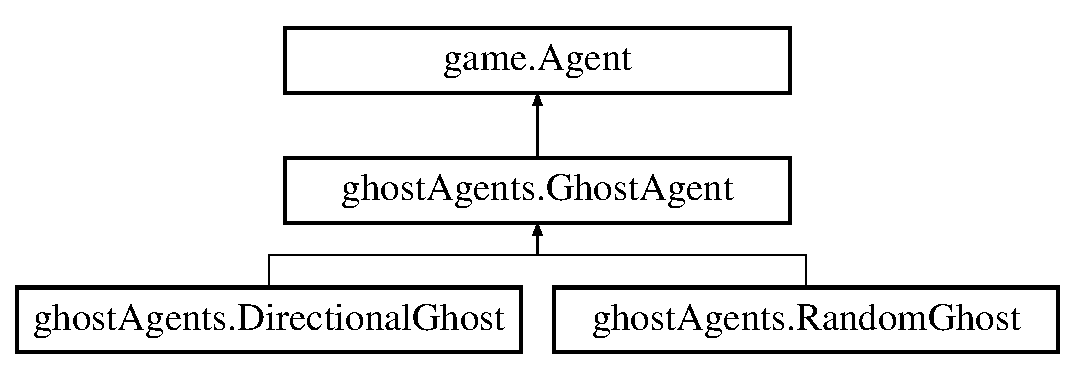
\includegraphics[height=3.000000cm]{classghost_agents_1_1_ghost_agent}
\end{center}
\end{figure}
\subsection*{Public Member Functions}
\begin{DoxyCompactItemize}
\item 
\mbox{\Hypertarget{classghost_agents_1_1_ghost_agent_a310fa4e78fec0b7667ff6bcbcc54ad1e}\label{classghost_agents_1_1_ghost_agent_a310fa4e78fec0b7667ff6bcbcc54ad1e}} 
def {\bfseries \+\_\+\+\_\+init\+\_\+\+\_\+} (self, index)
\item 
\mbox{\Hypertarget{classghost_agents_1_1_ghost_agent_a2139653922c8efd6599b9c53b6ef0d9a}\label{classghost_agents_1_1_ghost_agent_a2139653922c8efd6599b9c53b6ef0d9a}} 
def {\bfseries get\+Action} (self, state)
\item 
\mbox{\Hypertarget{classghost_agents_1_1_ghost_agent_afb68eca205c88f32a9ec80e5f0c7adb3}\label{classghost_agents_1_1_ghost_agent_afb68eca205c88f32a9ec80e5f0c7adb3}} 
def {\bfseries get\+Distribution} (self, state)
\end{DoxyCompactItemize}
\subsection*{Public Attributes}
\begin{DoxyCompactItemize}
\item 
\mbox{\Hypertarget{classghost_agents_1_1_ghost_agent_a13192b8c0890659fd738af2c02cfd04c}\label{classghost_agents_1_1_ghost_agent_a13192b8c0890659fd738af2c02cfd04c}} 
{\bfseries index}
\end{DoxyCompactItemize}


The documentation for this class was generated from the following file\+:\begin{DoxyCompactItemize}
\item 
ghost\+Agents.\+py\end{DoxyCompactItemize}

\hypertarget{classpacman_1_1_ghost_rules}{}\section{pacman.\+Ghost\+Rules Class Reference}
\label{classpacman_1_1_ghost_rules}\index{pacman.\+Ghost\+Rules@{pacman.\+Ghost\+Rules}}
\subsection*{Public Member Functions}
\begin{DoxyCompactItemize}
\item 
def \hyperlink{classpacman_1_1_ghost_rules_a48577275f722505c68d595515c53859b}{get\+Legal\+Actions} (state, ghost\+Index)
\item 
\mbox{\Hypertarget{classpacman_1_1_ghost_rules_a37c28017fa5b59bc17ba6d580e4f0a21}\label{classpacman_1_1_ghost_rules_a37c28017fa5b59bc17ba6d580e4f0a21}} 
def {\bfseries apply\+Action} (state, action, ghost\+Index)
\item 
\mbox{\Hypertarget{classpacman_1_1_ghost_rules_aeaa76146bcebc36df5bb426159be884e}\label{classpacman_1_1_ghost_rules_aeaa76146bcebc36df5bb426159be884e}} 
def {\bfseries decrement\+Timer} (ghost\+State)
\item 
\mbox{\Hypertarget{classpacman_1_1_ghost_rules_a495c986813866509cd1985121e0f50c6}\label{classpacman_1_1_ghost_rules_a495c986813866509cd1985121e0f50c6}} 
def {\bfseries check\+Death} (state, agent\+Index)
\item 
\mbox{\Hypertarget{classpacman_1_1_ghost_rules_a9e1a57075b0fbf2d91721fccff6ec276}\label{classpacman_1_1_ghost_rules_a9e1a57075b0fbf2d91721fccff6ec276}} 
def {\bfseries collide} (state, ghost\+State, agent\+Index)
\item 
\mbox{\Hypertarget{classpacman_1_1_ghost_rules_a12f9bc228959d00755fbc3d7c6d99649}\label{classpacman_1_1_ghost_rules_a12f9bc228959d00755fbc3d7c6d99649}} 
def {\bfseries can\+Kill} (pacman\+Position, ghost\+Position)
\item 
\mbox{\Hypertarget{classpacman_1_1_ghost_rules_aece2f6e41fe172273fd634b54eabcec0}\label{classpacman_1_1_ghost_rules_aece2f6e41fe172273fd634b54eabcec0}} 
def {\bfseries place\+Ghost} (state, ghost\+State)
\end{DoxyCompactItemize}
\subsection*{Static Public Attributes}
\begin{DoxyCompactItemize}
\item 
\mbox{\Hypertarget{classpacman_1_1_ghost_rules_aebac2d1a41f6ab9264e4d1f96d34c5a7}\label{classpacman_1_1_ghost_rules_aebac2d1a41f6ab9264e4d1f96d34c5a7}} 
float {\bfseries G\+H\+O\+S\+T\+\_\+\+S\+P\+E\+ED} = 1.\+0
\item 
\mbox{\Hypertarget{classpacman_1_1_ghost_rules_a49be343751caa936de632344b5fea06c}\label{classpacman_1_1_ghost_rules_a49be343751caa936de632344b5fea06c}} 
{\bfseries get\+Legal\+Actions} = staticmethod( get\+Legal\+Actions )
\item 
\mbox{\Hypertarget{classpacman_1_1_ghost_rules_a886a1e7eb522fe15c2985a681ae56b1f}\label{classpacman_1_1_ghost_rules_a886a1e7eb522fe15c2985a681ae56b1f}} 
{\bfseries apply\+Action} = staticmethod( apply\+Action )
\item 
\mbox{\Hypertarget{classpacman_1_1_ghost_rules_ac6c43c3d3195b9a7e3c60161b32ef416}\label{classpacman_1_1_ghost_rules_ac6c43c3d3195b9a7e3c60161b32ef416}} 
{\bfseries decrement\+Timer} = staticmethod( decrement\+Timer )
\item 
\mbox{\Hypertarget{classpacman_1_1_ghost_rules_a451aa087637c3e9d853eb3b3ba8ae65e}\label{classpacman_1_1_ghost_rules_a451aa087637c3e9d853eb3b3ba8ae65e}} 
{\bfseries check\+Death} = staticmethod( check\+Death )
\item 
\mbox{\Hypertarget{classpacman_1_1_ghost_rules_a363ec0ec93ac5440a06de47d492f8450}\label{classpacman_1_1_ghost_rules_a363ec0ec93ac5440a06de47d492f8450}} 
{\bfseries collide} = staticmethod( collide )
\item 
\mbox{\Hypertarget{classpacman_1_1_ghost_rules_af7953fe487ff87de00c62ce368c2b67c}\label{classpacman_1_1_ghost_rules_af7953fe487ff87de00c62ce368c2b67c}} 
{\bfseries can\+Kill} = staticmethod( can\+Kill )
\item 
\mbox{\Hypertarget{classpacman_1_1_ghost_rules_ac6098b781cc1cc40a85441355a407a95}\label{classpacman_1_1_ghost_rules_ac6098b781cc1cc40a85441355a407a95}} 
{\bfseries place\+Ghost} = staticmethod( place\+Ghost )
\end{DoxyCompactItemize}


\subsection{Detailed Description}
\begin{DoxyVerb}These functions dictate how ghosts interact with their environment.
\end{DoxyVerb}
 

\subsection{Member Function Documentation}
\mbox{\Hypertarget{classpacman_1_1_ghost_rules_a48577275f722505c68d595515c53859b}\label{classpacman_1_1_ghost_rules_a48577275f722505c68d595515c53859b}} 
\index{pacman\+::\+Ghost\+Rules@{pacman\+::\+Ghost\+Rules}!get\+Legal\+Actions@{get\+Legal\+Actions}}
\index{get\+Legal\+Actions@{get\+Legal\+Actions}!pacman\+::\+Ghost\+Rules@{pacman\+::\+Ghost\+Rules}}
\subsubsection{\texorpdfstring{get\+Legal\+Actions()}{getLegalActions()}}
{\footnotesize\ttfamily def pacman.\+Ghost\+Rules.\+get\+Legal\+Actions (\begin{DoxyParamCaption}\item[{}]{state,  }\item[{}]{ghost\+Index }\end{DoxyParamCaption})}

\begin{DoxyVerb}Ghosts cannot stop, and cannot turn around unless they
reach a dead end, but can turn 90 degrees at intersections.
\end{DoxyVerb}
 

The documentation for this class was generated from the following file\+:\begin{DoxyCompactItemize}
\item 
pacman.\+py\end{DoxyCompactItemize}

\hypertarget{classsearch_agents_1_1_go_west_agent}{}\section{search\+Agents.\+Go\+West\+Agent Class Reference}
\label{classsearch_agents_1_1_go_west_agent}\index{search\+Agents.\+Go\+West\+Agent@{search\+Agents.\+Go\+West\+Agent}}
Inheritance diagram for search\+Agents.\+Go\+West\+Agent\+:\begin{figure}[H]
\begin{center}
\leavevmode
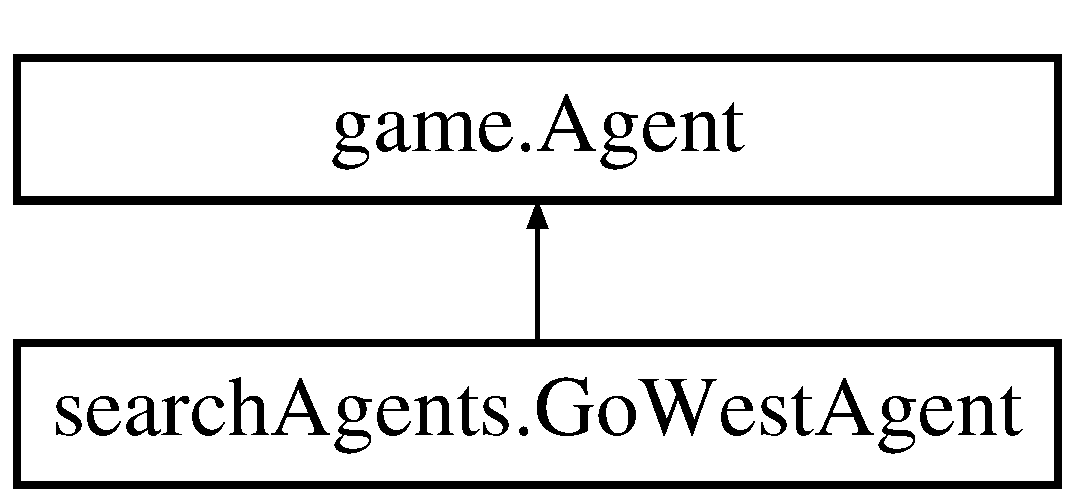
\includegraphics[height=2.000000cm]{classsearch_agents_1_1_go_west_agent}
\end{center}
\end{figure}
\subsection*{Public Member Functions}
\begin{DoxyCompactItemize}
\item 
\mbox{\Hypertarget{classsearch_agents_1_1_go_west_agent_a9388dd683a456db8643cbe65f37341cc}\label{classsearch_agents_1_1_go_west_agent_a9388dd683a456db8643cbe65f37341cc}} 
def {\bfseries get\+Action} (self, state)
\end{DoxyCompactItemize}
\subsection*{Additional Inherited Members}


The documentation for this class was generated from the following file\+:\begin{DoxyCompactItemize}
\item 
search\+Agents.\+py\end{DoxyCompactItemize}

\hypertarget{classpacman_agents_1_1_greedy_agent}{}\section{pacman\+Agents.\+Greedy\+Agent Class Reference}
\label{classpacman_agents_1_1_greedy_agent}\index{pacman\+Agents.\+Greedy\+Agent@{pacman\+Agents.\+Greedy\+Agent}}
Inheritance diagram for pacman\+Agents.\+Greedy\+Agent\+:\begin{figure}[H]
\begin{center}
\leavevmode
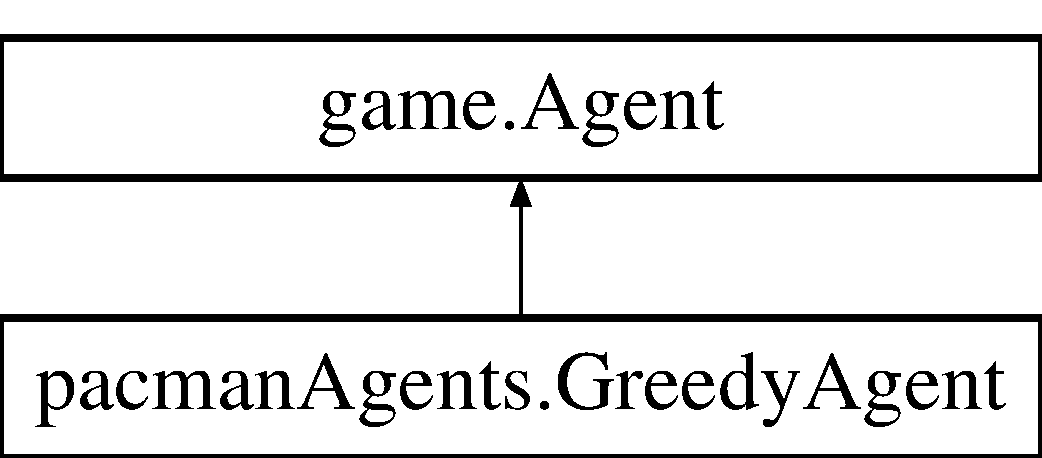
\includegraphics[height=2.000000cm]{classpacman_agents_1_1_greedy_agent}
\end{center}
\end{figure}
\subsection*{Public Member Functions}
\begin{DoxyCompactItemize}
\item 
\mbox{\Hypertarget{classpacman_agents_1_1_greedy_agent_ab1b3b7a06301b7382668a18ddcae3d73}\label{classpacman_agents_1_1_greedy_agent_ab1b3b7a06301b7382668a18ddcae3d73}} 
def {\bfseries \+\_\+\+\_\+init\+\_\+\+\_\+} (self, eval\+Fn=\char`\"{}score\+Evaluation\char`\"{})
\item 
\mbox{\Hypertarget{classpacman_agents_1_1_greedy_agent_a55f39125cdcb5c991ac8989b4ca9c4dd}\label{classpacman_agents_1_1_greedy_agent_a55f39125cdcb5c991ac8989b4ca9c4dd}} 
def {\bfseries get\+Action} (self, state)
\end{DoxyCompactItemize}
\subsection*{Public Attributes}
\begin{DoxyCompactItemize}
\item 
\mbox{\Hypertarget{classpacman_agents_1_1_greedy_agent_aa1bd3b90476cee8214e9b0a8f7109a01}\label{classpacman_agents_1_1_greedy_agent_aa1bd3b90476cee8214e9b0a8f7109a01}} 
{\bfseries evaluation\+Function}
\end{DoxyCompactItemize}


The documentation for this class was generated from the following file\+:\begin{DoxyCompactItemize}
\item 
pacman\+Agents.\+py\end{DoxyCompactItemize}

\hypertarget{classgame_1_1_grid}{}\section{game.\+Grid Class Reference}
\label{classgame_1_1_grid}\index{game.\+Grid@{game.\+Grid}}
\subsection*{Public Member Functions}
\begin{DoxyCompactItemize}
\item 
\mbox{\Hypertarget{classgame_1_1_grid_a3b1b83ba30899fe0c032e4c0c54742b5}\label{classgame_1_1_grid_a3b1b83ba30899fe0c032e4c0c54742b5}} 
def {\bfseries \+\_\+\+\_\+init\+\_\+\+\_\+} (self, width, height, initial\+Value=False, bit\+Representation=None)
\item 
\mbox{\Hypertarget{classgame_1_1_grid_ab510e1e89123ae205d1650456531a61b}\label{classgame_1_1_grid_ab510e1e89123ae205d1650456531a61b}} 
def {\bfseries \+\_\+\+\_\+getitem\+\_\+\+\_\+} (self, i)
\item 
\mbox{\Hypertarget{classgame_1_1_grid_a49d1ab55502c27cc282aedb477a1a9b1}\label{classgame_1_1_grid_a49d1ab55502c27cc282aedb477a1a9b1}} 
def {\bfseries \+\_\+\+\_\+setitem\+\_\+\+\_\+} (self, key, item)
\item 
\mbox{\Hypertarget{classgame_1_1_grid_a9386299c8dbfc9b670ed524b61d394c1}\label{classgame_1_1_grid_a9386299c8dbfc9b670ed524b61d394c1}} 
def {\bfseries \+\_\+\+\_\+str\+\_\+\+\_\+} (self)
\item 
\mbox{\Hypertarget{classgame_1_1_grid_a130cb4e409a9e69c9925c324b3c3c943}\label{classgame_1_1_grid_a130cb4e409a9e69c9925c324b3c3c943}} 
def {\bfseries \+\_\+\+\_\+eq\+\_\+\+\_\+} (self, other)
\item 
\mbox{\Hypertarget{classgame_1_1_grid_a6c182310c465b15d37a5971216285a06}\label{classgame_1_1_grid_a6c182310c465b15d37a5971216285a06}} 
def {\bfseries \+\_\+\+\_\+hash\+\_\+\+\_\+} (self)
\item 
\mbox{\Hypertarget{classgame_1_1_grid_a23c3c93e0813bf12635de17581d385da}\label{classgame_1_1_grid_a23c3c93e0813bf12635de17581d385da}} 
def {\bfseries copy} (self)
\item 
\mbox{\Hypertarget{classgame_1_1_grid_adcbc2f6d8ec7587b01df7aa2e060cb8d}\label{classgame_1_1_grid_adcbc2f6d8ec7587b01df7aa2e060cb8d}} 
def {\bfseries deep\+Copy} (self)
\item 
\mbox{\Hypertarget{classgame_1_1_grid_a1c2f255b295594d9fe01f6214ca3baec}\label{classgame_1_1_grid_a1c2f255b295594d9fe01f6214ca3baec}} 
def {\bfseries shallow\+Copy} (self)
\item 
\mbox{\Hypertarget{classgame_1_1_grid_a53de0c6dd98574c4e21aeb1df1a4c421}\label{classgame_1_1_grid_a53de0c6dd98574c4e21aeb1df1a4c421}} 
def {\bfseries count} (self, item=True)
\item 
\mbox{\Hypertarget{classgame_1_1_grid_a74e91d6f40cd3131c4c3541942cd45ba}\label{classgame_1_1_grid_a74e91d6f40cd3131c4c3541942cd45ba}} 
def {\bfseries as\+List} (self, key=True)
\item 
def \hyperlink{classgame_1_1_grid_a4cd22a6adb8a287be07ee4f09e623a2d}{pack\+Bits} (self)
\end{DoxyCompactItemize}
\subsection*{Public Attributes}
\begin{DoxyCompactItemize}
\item 
\mbox{\Hypertarget{classgame_1_1_grid_a1f1cd914b8cf1ff7caa66300968d1b55}\label{classgame_1_1_grid_a1f1cd914b8cf1ff7caa66300968d1b55}} 
{\bfseries C\+E\+L\+L\+S\+\_\+\+P\+E\+R\+\_\+\+I\+NT}
\item 
\mbox{\Hypertarget{classgame_1_1_grid_a106ada4249166c0c7ada9af0da1cace7}\label{classgame_1_1_grid_a106ada4249166c0c7ada9af0da1cace7}} 
{\bfseries width}
\item 
\mbox{\Hypertarget{classgame_1_1_grid_aaa8c96b31123ef167b4e2df70244174c}\label{classgame_1_1_grid_aaa8c96b31123ef167b4e2df70244174c}} 
{\bfseries height}
\item 
\mbox{\Hypertarget{classgame_1_1_grid_ae5f6f4dd2adda81b2db218c70a21694a}\label{classgame_1_1_grid_ae5f6f4dd2adda81b2db218c70a21694a}} 
{\bfseries data}
\end{DoxyCompactItemize}


\subsection{Detailed Description}
\begin{DoxyVerb}A 2-dimensional array of objects backed by a list of lists.  Data is accessed
via grid[x][y] where (x,y) are positions on a Pacman map with x horizontal,
y vertical and the origin (0,0) in the bottom left corner.

The __str__ method constructs an output that is oriented like a pacman board.
\end{DoxyVerb}
 

\subsection{Member Function Documentation}
\mbox{\Hypertarget{classgame_1_1_grid_a4cd22a6adb8a287be07ee4f09e623a2d}\label{classgame_1_1_grid_a4cd22a6adb8a287be07ee4f09e623a2d}} 
\index{game\+::\+Grid@{game\+::\+Grid}!pack\+Bits@{pack\+Bits}}
\index{pack\+Bits@{pack\+Bits}!game\+::\+Grid@{game\+::\+Grid}}
\subsubsection{\texorpdfstring{pack\+Bits()}{packBits()}}
{\footnotesize\ttfamily def game.\+Grid.\+pack\+Bits (\begin{DoxyParamCaption}\item[{}]{self }\end{DoxyParamCaption})}

\begin{DoxyVerb}Returns an efficient int list representation

(width, height, bitPackedInts...)
\end{DoxyVerb}
 

The documentation for this class was generated from the following file\+:\begin{DoxyCompactItemize}
\item 
game.\+py\end{DoxyCompactItemize}

\hypertarget{classgraphics_display_1_1_info_pane}{}\section{graphics\+Display.\+Info\+Pane Class Reference}
\label{classgraphics_display_1_1_info_pane}\index{graphics\+Display.\+Info\+Pane@{graphics\+Display.\+Info\+Pane}}
\subsection*{Public Member Functions}
\begin{DoxyCompactItemize}
\item 
\mbox{\Hypertarget{classgraphics_display_1_1_info_pane_aca3d7061176d3c4fa30ec5867402521b}\label{classgraphics_display_1_1_info_pane_aca3d7061176d3c4fa30ec5867402521b}} 
def {\bfseries \+\_\+\+\_\+init\+\_\+\+\_\+} (self, layout, grid\+Size)
\item 
def \hyperlink{classgraphics_display_1_1_info_pane_a187bf3ca47cd15c70a31d389463dfc62}{to\+Screen} (self, pos, y=None)
\item 
\mbox{\Hypertarget{classgraphics_display_1_1_info_pane_a8ab2aa721210b0c4fc4cf98725abfbb7}\label{classgraphics_display_1_1_info_pane_a8ab2aa721210b0c4fc4cf98725abfbb7}} 
def {\bfseries draw\+Pane} (self)
\item 
\mbox{\Hypertarget{classgraphics_display_1_1_info_pane_ac1ab4316ce7cab83076301d8d8c073a2}\label{classgraphics_display_1_1_info_pane_ac1ab4316ce7cab83076301d8d8c073a2}} 
def {\bfseries initialize\+Ghost\+Distances} (self, distances)
\item 
\mbox{\Hypertarget{classgraphics_display_1_1_info_pane_a9d4033159e219174a6ec86eb771d769b}\label{classgraphics_display_1_1_info_pane_a9d4033159e219174a6ec86eb771d769b}} 
def {\bfseries update\+Score} (self, score)
\item 
\mbox{\Hypertarget{classgraphics_display_1_1_info_pane_a9c14c0974008ee73bcab36130bf4c797}\label{classgraphics_display_1_1_info_pane_a9c14c0974008ee73bcab36130bf4c797}} 
def {\bfseries set\+Team} (self, is\+Blue)
\item 
\mbox{\Hypertarget{classgraphics_display_1_1_info_pane_a1fc130f47191c9db681003b5eb32e5f8}\label{classgraphics_display_1_1_info_pane_a1fc130f47191c9db681003b5eb32e5f8}} 
def {\bfseries update\+Ghost\+Distances} (self, distances)
\item 
\mbox{\Hypertarget{classgraphics_display_1_1_info_pane_a6d6f3620e86b4440ee59aa7cdddb81c8}\label{classgraphics_display_1_1_info_pane_a6d6f3620e86b4440ee59aa7cdddb81c8}} 
def {\bfseries draw\+Ghost} (self)
\item 
\mbox{\Hypertarget{classgraphics_display_1_1_info_pane_a1de4aa13f3c86313abf3aadc3997faa5}\label{classgraphics_display_1_1_info_pane_a1de4aa13f3c86313abf3aadc3997faa5}} 
def {\bfseries draw\+Pacman} (self)
\item 
\mbox{\Hypertarget{classgraphics_display_1_1_info_pane_aaea35dfa69d41ca7c99237840c70ad29}\label{classgraphics_display_1_1_info_pane_aaea35dfa69d41ca7c99237840c70ad29}} 
def {\bfseries draw\+Warning} (self)
\item 
\mbox{\Hypertarget{classgraphics_display_1_1_info_pane_a5156c9d17119c8134889138394de119e}\label{classgraphics_display_1_1_info_pane_a5156c9d17119c8134889138394de119e}} 
def {\bfseries clear\+Icon} (self)
\item 
\mbox{\Hypertarget{classgraphics_display_1_1_info_pane_af7fde70489bf993752d18b7721ffc514}\label{classgraphics_display_1_1_info_pane_af7fde70489bf993752d18b7721ffc514}} 
def {\bfseries update\+Message} (self, message)
\item 
\mbox{\Hypertarget{classgraphics_display_1_1_info_pane_a4c8899267718843696d75b6d4b898534}\label{classgraphics_display_1_1_info_pane_a4c8899267718843696d75b6d4b898534}} 
def {\bfseries clear\+Message} (self)
\end{DoxyCompactItemize}
\subsection*{Public Attributes}
\begin{DoxyCompactItemize}
\item 
\mbox{\Hypertarget{classgraphics_display_1_1_info_pane_af14473111b5ff56368287f7a15bfdc14}\label{classgraphics_display_1_1_info_pane_af14473111b5ff56368287f7a15bfdc14}} 
{\bfseries grid\+Size}
\item 
\mbox{\Hypertarget{classgraphics_display_1_1_info_pane_af75ef6c23a2e044eb774f646ce4e02e4}\label{classgraphics_display_1_1_info_pane_af75ef6c23a2e044eb774f646ce4e02e4}} 
{\bfseries width}
\item 
\mbox{\Hypertarget{classgraphics_display_1_1_info_pane_a02a632cc3e1297c7ddde3c7e56320633}\label{classgraphics_display_1_1_info_pane_a02a632cc3e1297c7ddde3c7e56320633}} 
{\bfseries base}
\item 
\mbox{\Hypertarget{classgraphics_display_1_1_info_pane_a518daef9e46b6f2078b6b567540ccf3c}\label{classgraphics_display_1_1_info_pane_a518daef9e46b6f2078b6b567540ccf3c}} 
{\bfseries height}
\item 
\mbox{\Hypertarget{classgraphics_display_1_1_info_pane_a19caafc08967904d2e64421d3af57fdb}\label{classgraphics_display_1_1_info_pane_a19caafc08967904d2e64421d3af57fdb}} 
{\bfseries font\+Size}
\item 
\mbox{\Hypertarget{classgraphics_display_1_1_info_pane_a1d8dd32873451c2feca70cd83e320074}\label{classgraphics_display_1_1_info_pane_a1d8dd32873451c2feca70cd83e320074}} 
{\bfseries text\+Color}
\item 
\mbox{\Hypertarget{classgraphics_display_1_1_info_pane_a3747d70eea5318a757a5209649048c51}\label{classgraphics_display_1_1_info_pane_a3747d70eea5318a757a5209649048c51}} 
{\bfseries score\+Text}
\item 
\mbox{\Hypertarget{classgraphics_display_1_1_info_pane_adad53bf1ebc476ca93da22db3ad183a9}\label{classgraphics_display_1_1_info_pane_adad53bf1ebc476ca93da22db3ad183a9}} 
{\bfseries ghost\+Distance\+Text}
\item 
\mbox{\Hypertarget{classgraphics_display_1_1_info_pane_a6092e91524243ab5fdc8af69fd2cea4d}\label{classgraphics_display_1_1_info_pane_a6092e91524243ab5fdc8af69fd2cea4d}} 
{\bfseries team\+Text}
\end{DoxyCompactItemize}


\subsection{Member Function Documentation}
\mbox{\Hypertarget{classgraphics_display_1_1_info_pane_a187bf3ca47cd15c70a31d389463dfc62}\label{classgraphics_display_1_1_info_pane_a187bf3ca47cd15c70a31d389463dfc62}} 
\index{graphics\+Display\+::\+Info\+Pane@{graphics\+Display\+::\+Info\+Pane}!to\+Screen@{to\+Screen}}
\index{to\+Screen@{to\+Screen}!graphics\+Display\+::\+Info\+Pane@{graphics\+Display\+::\+Info\+Pane}}
\subsubsection{\texorpdfstring{to\+Screen()}{toScreen()}}
{\footnotesize\ttfamily def graphics\+Display.\+Info\+Pane.\+to\+Screen (\begin{DoxyParamCaption}\item[{}]{self,  }\item[{}]{pos,  }\item[{}]{y = {\ttfamily None} }\end{DoxyParamCaption})}

\begin{DoxyVerb}  Translates a point relative from the bottom left of the info pane.
\end{DoxyVerb}
 

The documentation for this class was generated from the following file\+:\begin{DoxyCompactItemize}
\item 
graphics\+Display.\+py\end{DoxyCompactItemize}

\hypertarget{classkeyboard_agents_1_1_keyboard_agent}{}\section{keyboard\+Agents.\+Keyboard\+Agent Class Reference}
\label{classkeyboard_agents_1_1_keyboard_agent}\index{keyboard\+Agents.\+Keyboard\+Agent@{keyboard\+Agents.\+Keyboard\+Agent}}
Inheritance diagram for keyboard\+Agents.\+Keyboard\+Agent\+:\begin{figure}[H]
\begin{center}
\leavevmode
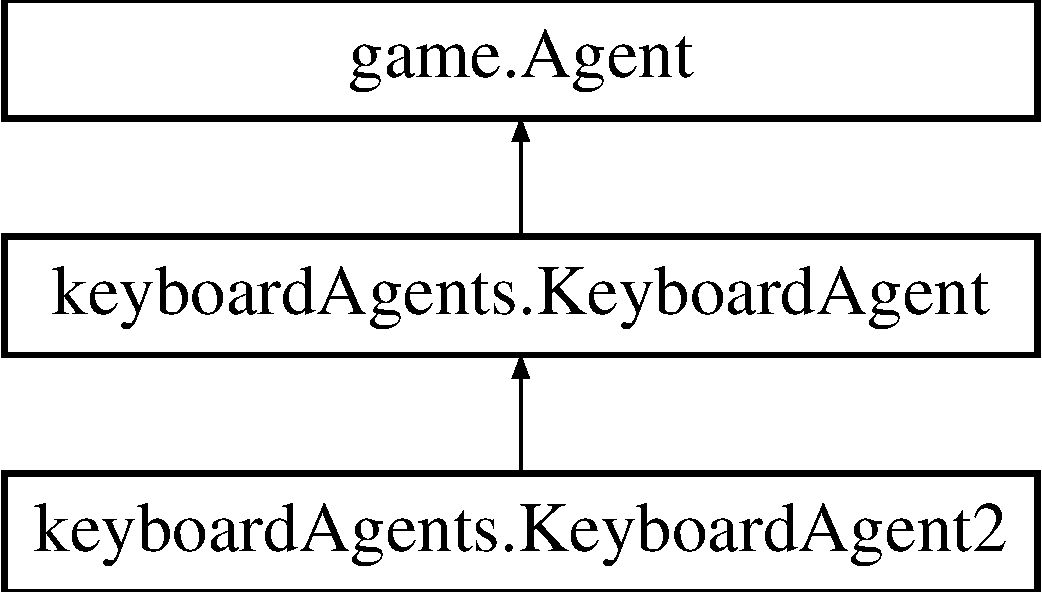
\includegraphics[height=3.000000cm]{classkeyboard_agents_1_1_keyboard_agent}
\end{center}
\end{figure}
\subsection*{Public Member Functions}
\begin{DoxyCompactItemize}
\item 
\mbox{\Hypertarget{classkeyboard_agents_1_1_keyboard_agent_a7f3e347791daf272729ef327c851a1d2}\label{classkeyboard_agents_1_1_keyboard_agent_a7f3e347791daf272729ef327c851a1d2}} 
def {\bfseries \+\_\+\+\_\+init\+\_\+\+\_\+} (self, index=0)
\item 
\mbox{\Hypertarget{classkeyboard_agents_1_1_keyboard_agent_ab543dae39f1789b6e3977d8020a8b057}\label{classkeyboard_agents_1_1_keyboard_agent_ab543dae39f1789b6e3977d8020a8b057}} 
def {\bfseries get\+Action} (self, state)
\item 
\mbox{\Hypertarget{classkeyboard_agents_1_1_keyboard_agent_a7bfbb5a2ac852a82c1ec237e7a197567}\label{classkeyboard_agents_1_1_keyboard_agent_a7bfbb5a2ac852a82c1ec237e7a197567}} 
def {\bfseries get\+Move} (self, legal)
\end{DoxyCompactItemize}
\subsection*{Public Attributes}
\begin{DoxyCompactItemize}
\item 
\mbox{\Hypertarget{classkeyboard_agents_1_1_keyboard_agent_a7565fe4c6dcd44fedae7679ad0ecd1b3}\label{classkeyboard_agents_1_1_keyboard_agent_a7565fe4c6dcd44fedae7679ad0ecd1b3}} 
{\bfseries last\+Move}
\item 
\mbox{\Hypertarget{classkeyboard_agents_1_1_keyboard_agent_a176bc9b6f308dd362f0483cbe8973c2f}\label{classkeyboard_agents_1_1_keyboard_agent_a176bc9b6f308dd362f0483cbe8973c2f}} 
{\bfseries index}
\item 
\mbox{\Hypertarget{classkeyboard_agents_1_1_keyboard_agent_a5a5b9646d55b8c7f3ca5f94507750e94}\label{classkeyboard_agents_1_1_keyboard_agent_a5a5b9646d55b8c7f3ca5f94507750e94}} 
{\bfseries keys}
\end{DoxyCompactItemize}
\subsection*{Static Public Attributes}
\begin{DoxyCompactItemize}
\item 
\mbox{\Hypertarget{classkeyboard_agents_1_1_keyboard_agent_a87be222de2f75014dec16cc6e8b463e6}\label{classkeyboard_agents_1_1_keyboard_agent_a87be222de2f75014dec16cc6e8b463e6}} 
string {\bfseries W\+E\+S\+T\+\_\+\+K\+EY} = \textquotesingle{}a\textquotesingle{}
\item 
\mbox{\Hypertarget{classkeyboard_agents_1_1_keyboard_agent_a691a87037816ea97841c435b1d3cf1cf}\label{classkeyboard_agents_1_1_keyboard_agent_a691a87037816ea97841c435b1d3cf1cf}} 
string {\bfseries E\+A\+S\+T\+\_\+\+K\+EY} = \textquotesingle{}d\textquotesingle{}
\item 
\mbox{\Hypertarget{classkeyboard_agents_1_1_keyboard_agent_a05e99895a700f1303a035a4c39bd7762}\label{classkeyboard_agents_1_1_keyboard_agent_a05e99895a700f1303a035a4c39bd7762}} 
string {\bfseries N\+O\+R\+T\+H\+\_\+\+K\+EY} = \textquotesingle{}w\textquotesingle{}
\item 
\mbox{\Hypertarget{classkeyboard_agents_1_1_keyboard_agent_a3f32ee636819f2c4655d086d6890d4f0}\label{classkeyboard_agents_1_1_keyboard_agent_a3f32ee636819f2c4655d086d6890d4f0}} 
string {\bfseries S\+O\+U\+T\+H\+\_\+\+K\+EY} = \textquotesingle{}s\textquotesingle{}
\item 
\mbox{\Hypertarget{classkeyboard_agents_1_1_keyboard_agent_ad96eebc75e3ac5028a2b60abed0e48f1}\label{classkeyboard_agents_1_1_keyboard_agent_ad96eebc75e3ac5028a2b60abed0e48f1}} 
string {\bfseries S\+T\+O\+P\+\_\+\+K\+EY} = \textquotesingle{}q\textquotesingle{}
\end{DoxyCompactItemize}


\subsection{Detailed Description}
\begin{DoxyVerb}An agent controlled by the keyboard.
\end{DoxyVerb}
 

The documentation for this class was generated from the following file\+:\begin{DoxyCompactItemize}
\item 
keyboard\+Agents.\+py\end{DoxyCompactItemize}

\hypertarget{classkeyboard_agents_1_1_keyboard_agent2}{}\section{keyboard\+Agents.\+Keyboard\+Agent2 Class Reference}
\label{classkeyboard_agents_1_1_keyboard_agent2}\index{keyboard\+Agents.\+Keyboard\+Agent2@{keyboard\+Agents.\+Keyboard\+Agent2}}
Inheritance diagram for keyboard\+Agents.\+Keyboard\+Agent2\+:\begin{figure}[H]
\begin{center}
\leavevmode
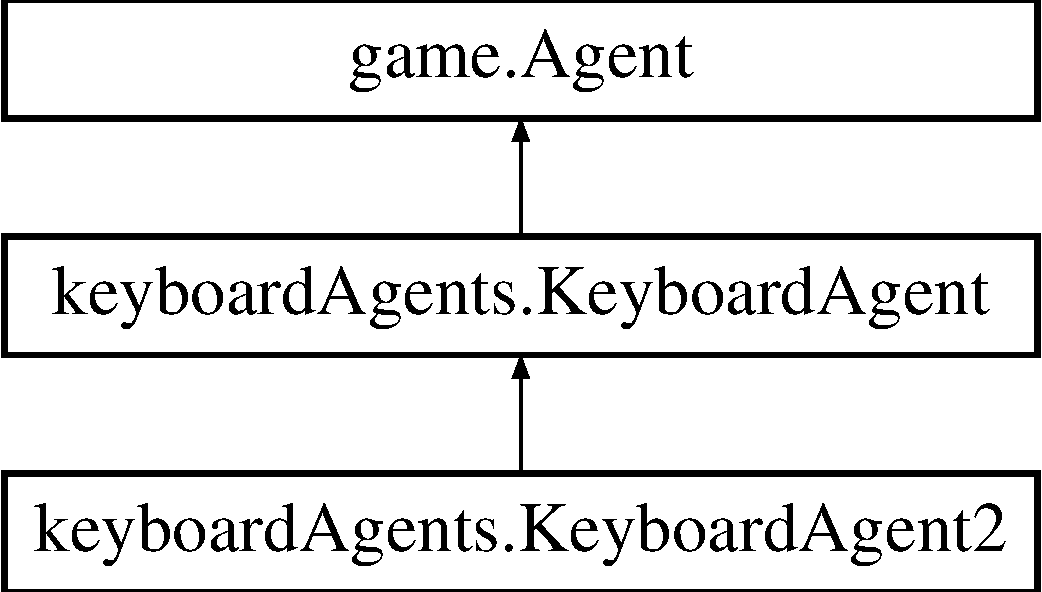
\includegraphics[height=3.000000cm]{classkeyboard_agents_1_1_keyboard_agent2}
\end{center}
\end{figure}
\subsection*{Public Member Functions}
\begin{DoxyCompactItemize}
\item 
\mbox{\Hypertarget{classkeyboard_agents_1_1_keyboard_agent2_a31d5f7e4cb4b593d397d749542e2f506}\label{classkeyboard_agents_1_1_keyboard_agent2_a31d5f7e4cb4b593d397d749542e2f506}} 
def {\bfseries get\+Move} (self, legal)
\end{DoxyCompactItemize}
\subsection*{Static Public Attributes}
\begin{DoxyCompactItemize}
\item 
\mbox{\Hypertarget{classkeyboard_agents_1_1_keyboard_agent2_aa3ef988d9fd4dd6332e6bafc5d7b0394}\label{classkeyboard_agents_1_1_keyboard_agent2_aa3ef988d9fd4dd6332e6bafc5d7b0394}} 
string {\bfseries W\+E\+S\+T\+\_\+\+K\+EY} = \textquotesingle{}j\textquotesingle{}
\item 
\mbox{\Hypertarget{classkeyboard_agents_1_1_keyboard_agent2_aaa3cb5f4c39f3a3f0db6f5f2b84edd56}\label{classkeyboard_agents_1_1_keyboard_agent2_aaa3cb5f4c39f3a3f0db6f5f2b84edd56}} 
string {\bfseries E\+A\+S\+T\+\_\+\+K\+EY} = \char`\"{}l\char`\"{}
\item 
\mbox{\Hypertarget{classkeyboard_agents_1_1_keyboard_agent2_a57c2562b51c56b8233076a44c4b6f014}\label{classkeyboard_agents_1_1_keyboard_agent2_a57c2562b51c56b8233076a44c4b6f014}} 
string {\bfseries N\+O\+R\+T\+H\+\_\+\+K\+EY} = \textquotesingle{}i\textquotesingle{}
\item 
\mbox{\Hypertarget{classkeyboard_agents_1_1_keyboard_agent2_a50e5d60e42d3c1ac22c3f9e36dac32af}\label{classkeyboard_agents_1_1_keyboard_agent2_a50e5d60e42d3c1ac22c3f9e36dac32af}} 
string {\bfseries S\+O\+U\+T\+H\+\_\+\+K\+EY} = \textquotesingle{}k\textquotesingle{}
\item 
\mbox{\Hypertarget{classkeyboard_agents_1_1_keyboard_agent2_a7ce3b23fb9b986174e839064dff885f5}\label{classkeyboard_agents_1_1_keyboard_agent2_a7ce3b23fb9b986174e839064dff885f5}} 
string {\bfseries S\+T\+O\+P\+\_\+\+K\+EY} = \textquotesingle{}u\textquotesingle{}
\end{DoxyCompactItemize}
\subsection*{Additional Inherited Members}


\subsection{Detailed Description}
\begin{DoxyVerb}A second agent controlled by the keyboard.
\end{DoxyVerb}
 

The documentation for this class was generated from the following file\+:\begin{DoxyCompactItemize}
\item 
keyboard\+Agents.\+py\end{DoxyCompactItemize}

\hypertarget{classlayout_1_1_layout}{}\section{layout.\+Layout Class Reference}
\label{classlayout_1_1_layout}\index{layout.\+Layout@{layout.\+Layout}}
\subsection*{Public Member Functions}
\begin{DoxyCompactItemize}
\item 
\mbox{\Hypertarget{classlayout_1_1_layout_a9315188e463c2a392e9ffbd56d4905cb}\label{classlayout_1_1_layout_a9315188e463c2a392e9ffbd56d4905cb}} 
def {\bfseries \+\_\+\+\_\+init\+\_\+\+\_\+} (self, layout\+Text)
\item 
\mbox{\Hypertarget{classlayout_1_1_layout_adc4a2a5c6766df70656b82735233658b}\label{classlayout_1_1_layout_adc4a2a5c6766df70656b82735233658b}} 
def {\bfseries get\+Num\+Ghosts} (self)
\item 
\mbox{\Hypertarget{classlayout_1_1_layout_abe375dbaeb7a51ba9084a2f68be9e8a9}\label{classlayout_1_1_layout_abe375dbaeb7a51ba9084a2f68be9e8a9}} 
def {\bfseries initialize\+Visibility\+Matrix} (self)
\item 
\mbox{\Hypertarget{classlayout_1_1_layout_acfa1ebd690d85feca46f19b98bd0010d}\label{classlayout_1_1_layout_acfa1ebd690d85feca46f19b98bd0010d}} 
def {\bfseries is\+Wall} (self, pos)
\item 
\mbox{\Hypertarget{classlayout_1_1_layout_a5e0682daef5027cb2a1de90ee55df82d}\label{classlayout_1_1_layout_a5e0682daef5027cb2a1de90ee55df82d}} 
def {\bfseries get\+Random\+Legal\+Position} (self)
\item 
\mbox{\Hypertarget{classlayout_1_1_layout_a4508abb1e19f362186190d38d771b61b}\label{classlayout_1_1_layout_a4508abb1e19f362186190d38d771b61b}} 
def {\bfseries get\+Random\+Corner} (self)
\item 
\mbox{\Hypertarget{classlayout_1_1_layout_a74cb9bf2995079b0a014acb2e3621945}\label{classlayout_1_1_layout_a74cb9bf2995079b0a014acb2e3621945}} 
def {\bfseries get\+Furthest\+Corner} (self, pac\+Pos)
\item 
\mbox{\Hypertarget{classlayout_1_1_layout_a0cfafa0bf7e8db7dd59b5a887db260c5}\label{classlayout_1_1_layout_a0cfafa0bf7e8db7dd59b5a887db260c5}} 
def {\bfseries is\+Visible\+From} (self, ghost\+Pos, pac\+Pos, pac\+Direction)
\item 
\mbox{\Hypertarget{classlayout_1_1_layout_a9dc7c8d1acb6584c10a193d6369a31c4}\label{classlayout_1_1_layout_a9dc7c8d1acb6584c10a193d6369a31c4}} 
def {\bfseries \+\_\+\+\_\+str\+\_\+\+\_\+} (self)
\item 
\mbox{\Hypertarget{classlayout_1_1_layout_aebbd593a1d9ac45c3c3e1a82926de076}\label{classlayout_1_1_layout_aebbd593a1d9ac45c3c3e1a82926de076}} 
def {\bfseries deep\+Copy} (self)
\item 
def \hyperlink{classlayout_1_1_layout_a4e7437180be84096a4352067707318eb}{process\+Layout\+Text} (self, layout\+Text)
\item 
\mbox{\Hypertarget{classlayout_1_1_layout_a3f337d339f7a34f1f7149b43091c9607}\label{classlayout_1_1_layout_a3f337d339f7a34f1f7149b43091c9607}} 
def {\bfseries process\+Layout\+Char} (self, x, y, layout\+Char)
\end{DoxyCompactItemize}
\subsection*{Public Attributes}
\begin{DoxyCompactItemize}
\item 
\mbox{\Hypertarget{classlayout_1_1_layout_ae1f581ae0a8470e37f0073a010a13880}\label{classlayout_1_1_layout_ae1f581ae0a8470e37f0073a010a13880}} 
{\bfseries width}
\item 
\mbox{\Hypertarget{classlayout_1_1_layout_a1240dd71a3c0fbd34c7298d91a840df1}\label{classlayout_1_1_layout_a1240dd71a3c0fbd34c7298d91a840df1}} 
{\bfseries height}
\item 
\mbox{\Hypertarget{classlayout_1_1_layout_acfe8131363e76df140f8da2a1c4b8a7a}\label{classlayout_1_1_layout_acfe8131363e76df140f8da2a1c4b8a7a}} 
{\bfseries walls}
\item 
\mbox{\Hypertarget{classlayout_1_1_layout_accd46c3abae6c892d74d79e919b31f81}\label{classlayout_1_1_layout_accd46c3abae6c892d74d79e919b31f81}} 
{\bfseries food}
\item 
\mbox{\Hypertarget{classlayout_1_1_layout_af0c5f58aa7c5a7b66fdb4926a8ac441f}\label{classlayout_1_1_layout_af0c5f58aa7c5a7b66fdb4926a8ac441f}} 
{\bfseries capsules}
\item 
\mbox{\Hypertarget{classlayout_1_1_layout_ab2246a2777b806f8f4344fb25063cfe7}\label{classlayout_1_1_layout_ab2246a2777b806f8f4344fb25063cfe7}} 
{\bfseries agent\+Positions}
\item 
\mbox{\Hypertarget{classlayout_1_1_layout_a5ab246ebcd9541a880d87523f57dee5c}\label{classlayout_1_1_layout_a5ab246ebcd9541a880d87523f57dee5c}} 
{\bfseries num\+Ghosts}
\item 
\mbox{\Hypertarget{classlayout_1_1_layout_a1ccbddeb86f90301f41e3cd8b6c58661}\label{classlayout_1_1_layout_a1ccbddeb86f90301f41e3cd8b6c58661}} 
{\bfseries layout\+Text}
\item 
\mbox{\Hypertarget{classlayout_1_1_layout_a2cfd77f7fa177e9c96992cad586aa879}\label{classlayout_1_1_layout_a2cfd77f7fa177e9c96992cad586aa879}} 
{\bfseries visibility}
\end{DoxyCompactItemize}


\subsection{Detailed Description}
\begin{DoxyVerb}A Layout manages the static information about the game board.
\end{DoxyVerb}
 

\subsection{Member Function Documentation}
\mbox{\Hypertarget{classlayout_1_1_layout_a4e7437180be84096a4352067707318eb}\label{classlayout_1_1_layout_a4e7437180be84096a4352067707318eb}} 
\index{layout\+::\+Layout@{layout\+::\+Layout}!process\+Layout\+Text@{process\+Layout\+Text}}
\index{process\+Layout\+Text@{process\+Layout\+Text}!layout\+::\+Layout@{layout\+::\+Layout}}
\subsubsection{\texorpdfstring{process\+Layout\+Text()}{processLayoutText()}}
{\footnotesize\ttfamily def layout.\+Layout.\+process\+Layout\+Text (\begin{DoxyParamCaption}\item[{}]{self,  }\item[{}]{layout\+Text }\end{DoxyParamCaption})}

\begin{DoxyVerb}Coordinates are flipped from the input format to the (x,y) convention here

The shape of the maze.  Each character  
represents a different type of object.   
 % - Wall                               
 . - Food
 o - Capsule
 G - Ghost
 P - Pacman
Other characters are ignored.
\end{DoxyVerb}
 

The documentation for this class was generated from the following file\+:\begin{DoxyCompactItemize}
\item 
layout.\+py\end{DoxyCompactItemize}

\hypertarget{classpacman_agents_1_1_left_turn_agent}{}\section{pacman\+Agents.\+Left\+Turn\+Agent Class Reference}
\label{classpacman_agents_1_1_left_turn_agent}\index{pacman\+Agents.\+Left\+Turn\+Agent@{pacman\+Agents.\+Left\+Turn\+Agent}}
Inheritance diagram for pacman\+Agents.\+Left\+Turn\+Agent\+:\begin{figure}[H]
\begin{center}
\leavevmode
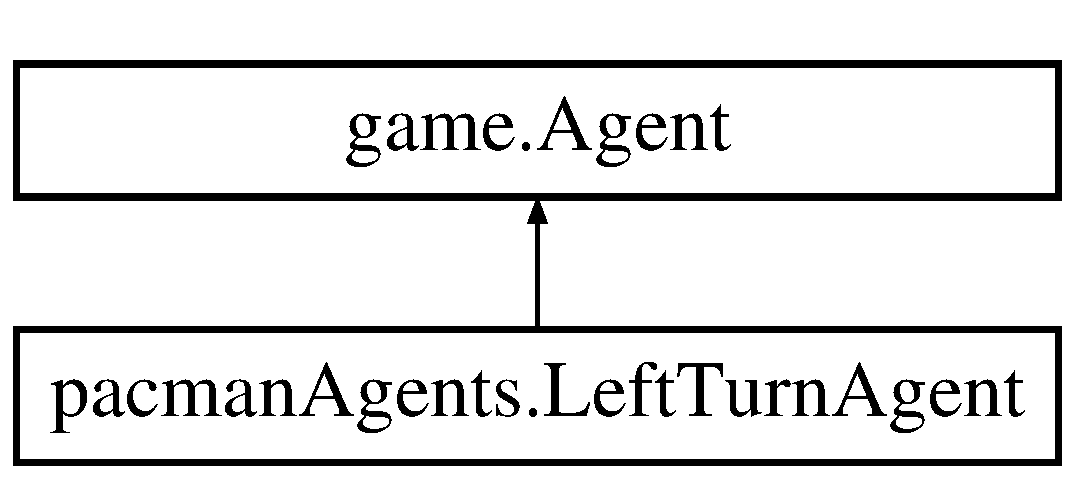
\includegraphics[height=2.000000cm]{classpacman_agents_1_1_left_turn_agent}
\end{center}
\end{figure}
\subsection*{Public Member Functions}
\begin{DoxyCompactItemize}
\item 
\mbox{\Hypertarget{classpacman_agents_1_1_left_turn_agent_a43d1804ba0a400dd83272ad3f634abc1}\label{classpacman_agents_1_1_left_turn_agent_a43d1804ba0a400dd83272ad3f634abc1}} 
def {\bfseries get\+Action} (self, state)
\end{DoxyCompactItemize}
\subsection*{Additional Inherited Members}


The documentation for this class was generated from the following file\+:\begin{DoxyCompactItemize}
\item 
pacman\+Agents.\+py\end{DoxyCompactItemize}

\hypertarget{classtext_display_1_1_null_graphics}{}\section{text\+Display.\+Null\+Graphics Class Reference}
\label{classtext_display_1_1_null_graphics}\index{text\+Display.\+Null\+Graphics@{text\+Display.\+Null\+Graphics}}
\subsection*{Public Member Functions}
\begin{DoxyCompactItemize}
\item 
\mbox{\Hypertarget{classtext_display_1_1_null_graphics_a15d4fa88ba93d27cf1342214e4f75473}\label{classtext_display_1_1_null_graphics_a15d4fa88ba93d27cf1342214e4f75473}} 
def {\bfseries initialize} (self, state, is\+Blue=False)
\item 
\mbox{\Hypertarget{classtext_display_1_1_null_graphics_ab4a92614b259e35d388ea5aeed5872d6}\label{classtext_display_1_1_null_graphics_ab4a92614b259e35d388ea5aeed5872d6}} 
def {\bfseries update} (self, state)
\item 
\mbox{\Hypertarget{classtext_display_1_1_null_graphics_a4243d7efb99c6aed25ac3017cede8666}\label{classtext_display_1_1_null_graphics_a4243d7efb99c6aed25ac3017cede8666}} 
def {\bfseries pause} (self)
\item 
\mbox{\Hypertarget{classtext_display_1_1_null_graphics_a4d4204bef8e5415f173d58ca4ae6a4a9}\label{classtext_display_1_1_null_graphics_a4d4204bef8e5415f173d58ca4ae6a4a9}} 
def {\bfseries draw} (self, state)
\item 
\mbox{\Hypertarget{classtext_display_1_1_null_graphics_a34f8876adf514cb304a3697dd128d552}\label{classtext_display_1_1_null_graphics_a34f8876adf514cb304a3697dd128d552}} 
def {\bfseries finish} (self)
\end{DoxyCompactItemize}


The documentation for this class was generated from the following file\+:\begin{DoxyCompactItemize}
\item 
text\+Display.\+py\end{DoxyCompactItemize}

\hypertarget{classtext_display_1_1_pacman_graphics}{}\section{text\+Display.\+Pacman\+Graphics Class Reference}
\label{classtext_display_1_1_pacman_graphics}\index{text\+Display.\+Pacman\+Graphics@{text\+Display.\+Pacman\+Graphics}}
\subsection*{Public Member Functions}
\begin{DoxyCompactItemize}
\item 
\mbox{\Hypertarget{classtext_display_1_1_pacman_graphics_a2a53cc3f0e6e5481e370429f7f714239}\label{classtext_display_1_1_pacman_graphics_a2a53cc3f0e6e5481e370429f7f714239}} 
def {\bfseries \+\_\+\+\_\+init\+\_\+\+\_\+} (self, speed=None)
\item 
\mbox{\Hypertarget{classtext_display_1_1_pacman_graphics_ae4253aa0a95b7a17d7536781a78e4d2e}\label{classtext_display_1_1_pacman_graphics_ae4253aa0a95b7a17d7536781a78e4d2e}} 
def {\bfseries initialize} (self, state, is\+Blue=False)
\item 
\mbox{\Hypertarget{classtext_display_1_1_pacman_graphics_a431f581ebd8d2cf60950edc516f4360b}\label{classtext_display_1_1_pacman_graphics_a431f581ebd8d2cf60950edc516f4360b}} 
def {\bfseries update} (self, state)
\item 
\mbox{\Hypertarget{classtext_display_1_1_pacman_graphics_ac0eb1250e27709f4efc2551743bfa042}\label{classtext_display_1_1_pacman_graphics_ac0eb1250e27709f4efc2551743bfa042}} 
def {\bfseries pause} (self)
\item 
\mbox{\Hypertarget{classtext_display_1_1_pacman_graphics_a2d230bfc90373966580443ce18bc7f01}\label{classtext_display_1_1_pacman_graphics_a2d230bfc90373966580443ce18bc7f01}} 
def {\bfseries draw} (self, state)
\item 
\mbox{\Hypertarget{classtext_display_1_1_pacman_graphics_a3f5ce6c054c157205caf55f62c926619}\label{classtext_display_1_1_pacman_graphics_a3f5ce6c054c157205caf55f62c926619}} 
def {\bfseries finish} (self)
\end{DoxyCompactItemize}
\subsection*{Public Attributes}
\begin{DoxyCompactItemize}
\item 
\mbox{\Hypertarget{classtext_display_1_1_pacman_graphics_ad590b9cef8434051027a2ef04346dad5}\label{classtext_display_1_1_pacman_graphics_ad590b9cef8434051027a2ef04346dad5}} 
{\bfseries turn}
\item 
\mbox{\Hypertarget{classtext_display_1_1_pacman_graphics_af360ec76080002ef0e1c1b2f57b7cef4}\label{classtext_display_1_1_pacman_graphics_af360ec76080002ef0e1c1b2f57b7cef4}} 
{\bfseries agent\+Counter}
\end{DoxyCompactItemize}


The documentation for this class was generated from the following file\+:\begin{DoxyCompactItemize}
\item 
text\+Display.\+py\end{DoxyCompactItemize}

\hypertarget{classgraphics_display_1_1_pacman_graphics}{}\section{graphics\+Display.\+Pacman\+Graphics Class Reference}
\label{classgraphics_display_1_1_pacman_graphics}\index{graphics\+Display.\+Pacman\+Graphics@{graphics\+Display.\+Pacman\+Graphics}}
Inheritance diagram for graphics\+Display.\+Pacman\+Graphics\+:\begin{figure}[H]
\begin{center}
\leavevmode
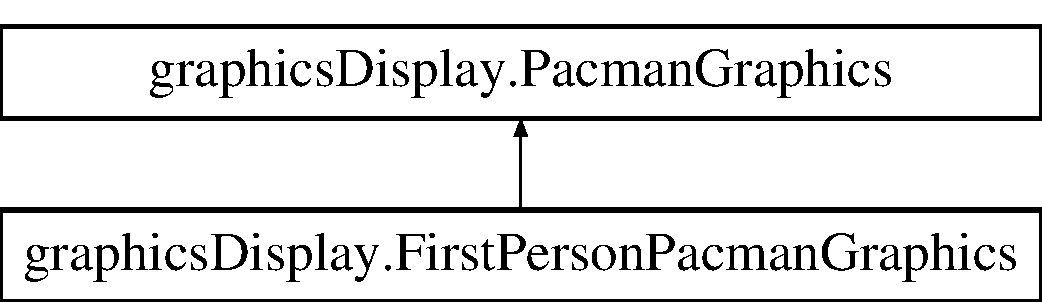
\includegraphics[height=2.000000cm]{classgraphics_display_1_1_pacman_graphics}
\end{center}
\end{figure}
\subsection*{Public Member Functions}
\begin{DoxyCompactItemize}
\item 
\mbox{\Hypertarget{classgraphics_display_1_1_pacman_graphics_a1f2ff5e46ad9142e430d1db50dc62fb3}\label{classgraphics_display_1_1_pacman_graphics_a1f2ff5e46ad9142e430d1db50dc62fb3}} 
def {\bfseries \+\_\+\+\_\+init\+\_\+\+\_\+} (self, zoom=1.\+0, frame\+Time=0.\+0, capture=False)
\item 
\mbox{\Hypertarget{classgraphics_display_1_1_pacman_graphics_a2d797692da8672d6dbbf90686dc9d33c}\label{classgraphics_display_1_1_pacman_graphics_a2d797692da8672d6dbbf90686dc9d33c}} 
def {\bfseries initialize} (self, state, is\+Blue=False)
\item 
\mbox{\Hypertarget{classgraphics_display_1_1_pacman_graphics_a757ee12fb854deed038d1c8805c1173d}\label{classgraphics_display_1_1_pacman_graphics_a757ee12fb854deed038d1c8805c1173d}} 
def {\bfseries start\+Graphics} (self, state)
\item 
\mbox{\Hypertarget{classgraphics_display_1_1_pacman_graphics_af9909fdb51aed076e63cc8e52e125f3c}\label{classgraphics_display_1_1_pacman_graphics_af9909fdb51aed076e63cc8e52e125f3c}} 
def {\bfseries draw\+Distributions} (self, state)
\item 
\mbox{\Hypertarget{classgraphics_display_1_1_pacman_graphics_a7cc7858ce3f72db75ffbb9bc3652578c}\label{classgraphics_display_1_1_pacman_graphics_a7cc7858ce3f72db75ffbb9bc3652578c}} 
def {\bfseries draw\+Static\+Objects} (self, state)
\item 
\mbox{\Hypertarget{classgraphics_display_1_1_pacman_graphics_a8c3b8f95c2ea4a9c497bc6bfe7d0368a}\label{classgraphics_display_1_1_pacman_graphics_a8c3b8f95c2ea4a9c497bc6bfe7d0368a}} 
def {\bfseries draw\+Agent\+Objects} (self, state)
\item 
def \hyperlink{classgraphics_display_1_1_pacman_graphics_afa38cdde4141fb7f84b80983404f6ab0}{swap\+Images} (self, agent\+Index, new\+State)
\item 
\mbox{\Hypertarget{classgraphics_display_1_1_pacman_graphics_ad2344cf277b2d71ab9da78bdeecd489b}\label{classgraphics_display_1_1_pacman_graphics_ad2344cf277b2d71ab9da78bdeecd489b}} 
def {\bfseries update} (self, new\+State)
\item 
\mbox{\Hypertarget{classgraphics_display_1_1_pacman_graphics_a36fbd919ef70248db977e693074ed848}\label{classgraphics_display_1_1_pacman_graphics_a36fbd919ef70248db977e693074ed848}} 
def {\bfseries make\+\_\+window} (self, width, height)
\item 
\mbox{\Hypertarget{classgraphics_display_1_1_pacman_graphics_a2d3c8792a0f373190d40d093ba8d2955}\label{classgraphics_display_1_1_pacman_graphics_a2d3c8792a0f373190d40d093ba8d2955}} 
def {\bfseries draw\+Pacman} (self, pacman, index)
\item 
\mbox{\Hypertarget{classgraphics_display_1_1_pacman_graphics_a4b717eafb23f242ddedaa795471c3253}\label{classgraphics_display_1_1_pacman_graphics_a4b717eafb23f242ddedaa795471c3253}} 
def {\bfseries get\+Endpoints} (self, direction, position=(0, 0))
\item 
\mbox{\Hypertarget{classgraphics_display_1_1_pacman_graphics_a35e2df6f62735a6a38111524af7bede1}\label{classgraphics_display_1_1_pacman_graphics_a35e2df6f62735a6a38111524af7bede1}} 
def {\bfseries move\+Pacman} (self, position, direction, image)
\item 
\mbox{\Hypertarget{classgraphics_display_1_1_pacman_graphics_a3c5c3ac8fa716a1cecda0aa719ec907e}\label{classgraphics_display_1_1_pacman_graphics_a3c5c3ac8fa716a1cecda0aa719ec907e}} 
def {\bfseries animate\+Pacman} (self, pacman, prev\+Pacman, image)
\item 
\mbox{\Hypertarget{classgraphics_display_1_1_pacman_graphics_aa1ba3d9e8c9121cc94a77a51c3cfe439}\label{classgraphics_display_1_1_pacman_graphics_aa1ba3d9e8c9121cc94a77a51c3cfe439}} 
def {\bfseries get\+Ghost\+Color} (self, ghost, ghost\+Index)
\item 
\mbox{\Hypertarget{classgraphics_display_1_1_pacman_graphics_a5ae92dd9a341e486aca20e5e66e0030d}\label{classgraphics_display_1_1_pacman_graphics_a5ae92dd9a341e486aca20e5e66e0030d}} 
def {\bfseries draw\+Ghost} (self, ghost, agent\+Index)
\item 
\mbox{\Hypertarget{classgraphics_display_1_1_pacman_graphics_aa07a9f6bf3c41431c373f8b6d84bc7d4}\label{classgraphics_display_1_1_pacman_graphics_aa07a9f6bf3c41431c373f8b6d84bc7d4}} 
def {\bfseries move\+Eyes} (self, pos, dir, eyes)
\item 
\mbox{\Hypertarget{classgraphics_display_1_1_pacman_graphics_a0ed205d5b7f9f1b0813c944f8ac7ebc0}\label{classgraphics_display_1_1_pacman_graphics_a0ed205d5b7f9f1b0813c944f8ac7ebc0}} 
def {\bfseries move\+Ghost} (self, ghost, ghost\+Index, prev\+Ghost, ghost\+Image\+Parts)
\item 
\mbox{\Hypertarget{classgraphics_display_1_1_pacman_graphics_a00aca399e2ac5c297c03e008046f3e24}\label{classgraphics_display_1_1_pacman_graphics_a00aca399e2ac5c297c03e008046f3e24}} 
def {\bfseries get\+Position} (self, agent\+State)
\item 
\mbox{\Hypertarget{classgraphics_display_1_1_pacman_graphics_a9fde033f0bf70d5e95910ffe3896bb52}\label{classgraphics_display_1_1_pacman_graphics_a9fde033f0bf70d5e95910ffe3896bb52}} 
def {\bfseries get\+Direction} (self, agent\+State)
\item 
\mbox{\Hypertarget{classgraphics_display_1_1_pacman_graphics_a702b67f9d71c25bc8ed9ebadede0b9f3}\label{classgraphics_display_1_1_pacman_graphics_a702b67f9d71c25bc8ed9ebadede0b9f3}} 
def {\bfseries finish} (self)
\item 
\mbox{\Hypertarget{classgraphics_display_1_1_pacman_graphics_a3121c93084f5d390174e03c5bb8c9f4b}\label{classgraphics_display_1_1_pacman_graphics_a3121c93084f5d390174e03c5bb8c9f4b}} 
def {\bfseries to\+\_\+screen} (self, point)
\item 
\mbox{\Hypertarget{classgraphics_display_1_1_pacman_graphics_adda16a80985b9eb9bd3ef9252d8db67d}\label{classgraphics_display_1_1_pacman_graphics_adda16a80985b9eb9bd3ef9252d8db67d}} 
def {\bfseries to\+\_\+screen2} (self, point)
\item 
\mbox{\Hypertarget{classgraphics_display_1_1_pacman_graphics_a8f15572076460835e300795d8a762018}\label{classgraphics_display_1_1_pacman_graphics_a8f15572076460835e300795d8a762018}} 
def {\bfseries draw\+Walls} (self, wall\+Matrix)
\item 
\mbox{\Hypertarget{classgraphics_display_1_1_pacman_graphics_a059148894da37d0e349484f8bbaf9ca5}\label{classgraphics_display_1_1_pacman_graphics_a059148894da37d0e349484f8bbaf9ca5}} 
def {\bfseries is\+Wall} (self, x, y, walls)
\item 
\mbox{\Hypertarget{classgraphics_display_1_1_pacman_graphics_a5e73a7939de734223671a2888236f689}\label{classgraphics_display_1_1_pacman_graphics_a5e73a7939de734223671a2888236f689}} 
def {\bfseries draw\+Food} (self, food\+Matrix)
\item 
\mbox{\Hypertarget{classgraphics_display_1_1_pacman_graphics_a7dcea1083c01392a624df34f4f76de96}\label{classgraphics_display_1_1_pacman_graphics_a7dcea1083c01392a624df34f4f76de96}} 
def {\bfseries draw\+Capsules} (self, capsules)
\item 
\mbox{\Hypertarget{classgraphics_display_1_1_pacman_graphics_a55ce947b9b687aef8e071e8dcc24f6ff}\label{classgraphics_display_1_1_pacman_graphics_a55ce947b9b687aef8e071e8dcc24f6ff}} 
def {\bfseries remove\+Food} (self, cell, food\+Images)
\item 
\mbox{\Hypertarget{classgraphics_display_1_1_pacman_graphics_a20b4b9e970a473a7d8a4e9ff4f5b584e}\label{classgraphics_display_1_1_pacman_graphics_a20b4b9e970a473a7d8a4e9ff4f5b584e}} 
def {\bfseries remove\+Capsule} (self, cell, capsule\+Images)
\item 
def \hyperlink{classgraphics_display_1_1_pacman_graphics_a9097dacf55460e7a0c6a1b2c8f1a7346}{draw\+Expanded\+Cells} (self, cells)
\item 
\mbox{\Hypertarget{classgraphics_display_1_1_pacman_graphics_ae4f415c33b65793e33d2ca369e8556b4}\label{classgraphics_display_1_1_pacman_graphics_ae4f415c33b65793e33d2ca369e8556b4}} 
def {\bfseries clear\+Expanded\+Cells} (self)
\item 
\mbox{\Hypertarget{classgraphics_display_1_1_pacman_graphics_ae26e9ef2dea7f3cc59de2b0061dc33d3}\label{classgraphics_display_1_1_pacman_graphics_ae26e9ef2dea7f3cc59de2b0061dc33d3}} 
def {\bfseries update\+Distributions} (self, distributions)
\end{DoxyCompactItemize}
\subsection*{Public Attributes}
\begin{DoxyCompactItemize}
\item 
\mbox{\Hypertarget{classgraphics_display_1_1_pacman_graphics_aa916db99e77cd4e2f4e7aae433addac5}\label{classgraphics_display_1_1_pacman_graphics_aa916db99e77cd4e2f4e7aae433addac5}} 
{\bfseries have\+\_\+window}
\item 
\mbox{\Hypertarget{classgraphics_display_1_1_pacman_graphics_a7f69a4470491916ad69863838e20a082}\label{classgraphics_display_1_1_pacman_graphics_a7f69a4470491916ad69863838e20a082}} 
{\bfseries current\+Ghost\+Images}
\item 
\mbox{\Hypertarget{classgraphics_display_1_1_pacman_graphics_adda2da4b2d88bec8df0d8a0089bec972}\label{classgraphics_display_1_1_pacman_graphics_adda2da4b2d88bec8df0d8a0089bec972}} 
{\bfseries pacman\+Image}
\item 
\mbox{\Hypertarget{classgraphics_display_1_1_pacman_graphics_a367afa50a454ec05c9914e97a3780153}\label{classgraphics_display_1_1_pacman_graphics_a367afa50a454ec05c9914e97a3780153}} 
{\bfseries zoom}
\item 
\mbox{\Hypertarget{classgraphics_display_1_1_pacman_graphics_a4e4c7286aa4927662e242ab6a4b6c1e3}\label{classgraphics_display_1_1_pacman_graphics_a4e4c7286aa4927662e242ab6a4b6c1e3}} 
{\bfseries grid\+Size}
\item 
\mbox{\Hypertarget{classgraphics_display_1_1_pacman_graphics_ad1551d0fdcd806f7130bd4bf07b7c067}\label{classgraphics_display_1_1_pacman_graphics_ad1551d0fdcd806f7130bd4bf07b7c067}} 
{\bfseries capture}
\item 
\mbox{\Hypertarget{classgraphics_display_1_1_pacman_graphics_a7e81da313110af8db4609ecc83e2aba6}\label{classgraphics_display_1_1_pacman_graphics_a7e81da313110af8db4609ecc83e2aba6}} 
{\bfseries frame\+Time}
\item 
\mbox{\Hypertarget{classgraphics_display_1_1_pacman_graphics_a24847ee2f406529e5fa7a60c30de638a}\label{classgraphics_display_1_1_pacman_graphics_a24847ee2f406529e5fa7a60c30de638a}} 
{\bfseries is\+Blue}
\item 
\mbox{\Hypertarget{classgraphics_display_1_1_pacman_graphics_a67f0fd3b5af80044bdec44a79bb41ffe}\label{classgraphics_display_1_1_pacman_graphics_a67f0fd3b5af80044bdec44a79bb41ffe}} 
{\bfseries distribution\+Images}
\item 
\mbox{\Hypertarget{classgraphics_display_1_1_pacman_graphics_a0b18dc520fdd51cc8a75918426dbd65d}\label{classgraphics_display_1_1_pacman_graphics_a0b18dc520fdd51cc8a75918426dbd65d}} 
{\bfseries previous\+State}
\item 
\mbox{\Hypertarget{classgraphics_display_1_1_pacman_graphics_a7547dc10e1681f928e5964e05c34a3e7}\label{classgraphics_display_1_1_pacman_graphics_a7547dc10e1681f928e5964e05c34a3e7}} 
{\bfseries layout}
\item 
\mbox{\Hypertarget{classgraphics_display_1_1_pacman_graphics_a2c172a4b81d9e0b3ca1f40473b63dbba}\label{classgraphics_display_1_1_pacman_graphics_a2c172a4b81d9e0b3ca1f40473b63dbba}} 
{\bfseries width}
\item 
\mbox{\Hypertarget{classgraphics_display_1_1_pacman_graphics_a839e7cf921d412657c0f5168d664acfd}\label{classgraphics_display_1_1_pacman_graphics_a839e7cf921d412657c0f5168d664acfd}} 
{\bfseries height}
\item 
\mbox{\Hypertarget{classgraphics_display_1_1_pacman_graphics_aef5c7940c51dd4aa978f4ac313977ea5}\label{classgraphics_display_1_1_pacman_graphics_aef5c7940c51dd4aa978f4ac313977ea5}} 
{\bfseries info\+Pane}
\item 
\mbox{\Hypertarget{classgraphics_display_1_1_pacman_graphics_a47ee9049f213bb4f6d2dada0d9d17ed3}\label{classgraphics_display_1_1_pacman_graphics_a47ee9049f213bb4f6d2dada0d9d17ed3}} 
{\bfseries current\+State}
\item 
\mbox{\Hypertarget{classgraphics_display_1_1_pacman_graphics_ac7dfb44b300a496fd4601ee05796955e}\label{classgraphics_display_1_1_pacman_graphics_ac7dfb44b300a496fd4601ee05796955e}} 
{\bfseries food}
\item 
\mbox{\Hypertarget{classgraphics_display_1_1_pacman_graphics_ad8ec0a8dac44eb5ec1a347ec62995e4e}\label{classgraphics_display_1_1_pacman_graphics_ad8ec0a8dac44eb5ec1a347ec62995e4e}} 
{\bfseries capsules}
\item 
\mbox{\Hypertarget{classgraphics_display_1_1_pacman_graphics_a007fc16f04d2eedcc77cf1b491124aa3}\label{classgraphics_display_1_1_pacman_graphics_a007fc16f04d2eedcc77cf1b491124aa3}} 
{\bfseries agent\+Images}
\item 
\mbox{\Hypertarget{classgraphics_display_1_1_pacman_graphics_a299f32c0d4b8dd3e931207cea81208f0}\label{classgraphics_display_1_1_pacman_graphics_a299f32c0d4b8dd3e931207cea81208f0}} 
{\bfseries expanded\+Cells}
\end{DoxyCompactItemize}


\subsection{Member Function Documentation}
\mbox{\Hypertarget{classgraphics_display_1_1_pacman_graphics_a9097dacf55460e7a0c6a1b2c8f1a7346}\label{classgraphics_display_1_1_pacman_graphics_a9097dacf55460e7a0c6a1b2c8f1a7346}} 
\index{graphics\+Display\+::\+Pacman\+Graphics@{graphics\+Display\+::\+Pacman\+Graphics}!draw\+Expanded\+Cells@{draw\+Expanded\+Cells}}
\index{draw\+Expanded\+Cells@{draw\+Expanded\+Cells}!graphics\+Display\+::\+Pacman\+Graphics@{graphics\+Display\+::\+Pacman\+Graphics}}
\subsubsection{\texorpdfstring{draw\+Expanded\+Cells()}{drawExpandedCells()}}
{\footnotesize\ttfamily def graphics\+Display.\+Pacman\+Graphics.\+draw\+Expanded\+Cells (\begin{DoxyParamCaption}\item[{}]{self,  }\item[{}]{cells }\end{DoxyParamCaption})}

\begin{DoxyVerb}Draws an overlay of expanded grid positions for search agents
\end{DoxyVerb}
 \mbox{\Hypertarget{classgraphics_display_1_1_pacman_graphics_afa38cdde4141fb7f84b80983404f6ab0}\label{classgraphics_display_1_1_pacman_graphics_afa38cdde4141fb7f84b80983404f6ab0}} 
\index{graphics\+Display\+::\+Pacman\+Graphics@{graphics\+Display\+::\+Pacman\+Graphics}!swap\+Images@{swap\+Images}}
\index{swap\+Images@{swap\+Images}!graphics\+Display\+::\+Pacman\+Graphics@{graphics\+Display\+::\+Pacman\+Graphics}}
\subsubsection{\texorpdfstring{swap\+Images()}{swapImages()}}
{\footnotesize\ttfamily def graphics\+Display.\+Pacman\+Graphics.\+swap\+Images (\begin{DoxyParamCaption}\item[{}]{self,  }\item[{}]{agent\+Index,  }\item[{}]{new\+State }\end{DoxyParamCaption})}

\begin{DoxyVerb}  Changes an image from a ghost to a pacman or vis versa (for capture)
\end{DoxyVerb}
 

The documentation for this class was generated from the following file\+:\begin{DoxyCompactItemize}
\item 
graphics\+Display.\+py\end{DoxyCompactItemize}

\hypertarget{classpacman_1_1_pacman_rules}{}\section{pacman.\+Pacman\+Rules Class Reference}
\label{classpacman_1_1_pacman_rules}\index{pacman.\+Pacman\+Rules@{pacman.\+Pacman\+Rules}}
\subsection*{Public Member Functions}
\begin{DoxyCompactItemize}
\item 
def \hyperlink{classpacman_1_1_pacman_rules_a515c73c403fdb8e7512bb9c587249477}{get\+Legal\+Actions} (state)
\item 
def \hyperlink{classpacman_1_1_pacman_rules_a8ba8b14554cc3631ad7ff93c973ba072}{apply\+Action} (state, action)
\item 
\mbox{\Hypertarget{classpacman_1_1_pacman_rules_a034aebb68831db2f8731c370548e4394}\label{classpacman_1_1_pacman_rules_a034aebb68831db2f8731c370548e4394}} 
def {\bfseries consume} (position, state)
\end{DoxyCompactItemize}
\subsection*{Static Public Attributes}
\begin{DoxyCompactItemize}
\item 
\mbox{\Hypertarget{classpacman_1_1_pacman_rules_a4deeb7c192985f7da2c210967f644a43}\label{classpacman_1_1_pacman_rules_a4deeb7c192985f7da2c210967f644a43}} 
int {\bfseries P\+A\+C\+M\+A\+N\+\_\+\+S\+P\+E\+ED} = 1
\item 
\mbox{\Hypertarget{classpacman_1_1_pacman_rules_a523da7c010db12bdb53772a5fdb47916}\label{classpacman_1_1_pacman_rules_a523da7c010db12bdb53772a5fdb47916}} 
{\bfseries get\+Legal\+Actions} = staticmethod( get\+Legal\+Actions )
\item 
\mbox{\Hypertarget{classpacman_1_1_pacman_rules_a703ce52c3a849ef9da084011e897d30f}\label{classpacman_1_1_pacman_rules_a703ce52c3a849ef9da084011e897d30f}} 
{\bfseries apply\+Action} = staticmethod( apply\+Action )
\item 
\mbox{\Hypertarget{classpacman_1_1_pacman_rules_a921c71dafaa0ee0caf9827fa15c1f9d1}\label{classpacman_1_1_pacman_rules_a921c71dafaa0ee0caf9827fa15c1f9d1}} 
{\bfseries consume} = staticmethod( consume )
\end{DoxyCompactItemize}


\subsection{Detailed Description}
\begin{DoxyVerb}These functions govern how pacman interacts with his environment under
the classic game rules.
\end{DoxyVerb}
 

\subsection{Member Function Documentation}
\mbox{\Hypertarget{classpacman_1_1_pacman_rules_a8ba8b14554cc3631ad7ff93c973ba072}\label{classpacman_1_1_pacman_rules_a8ba8b14554cc3631ad7ff93c973ba072}} 
\index{pacman\+::\+Pacman\+Rules@{pacman\+::\+Pacman\+Rules}!apply\+Action@{apply\+Action}}
\index{apply\+Action@{apply\+Action}!pacman\+::\+Pacman\+Rules@{pacman\+::\+Pacman\+Rules}}
\subsubsection{\texorpdfstring{apply\+Action()}{applyAction()}}
{\footnotesize\ttfamily def pacman.\+Pacman\+Rules.\+apply\+Action (\begin{DoxyParamCaption}\item[{}]{state,  }\item[{}]{action }\end{DoxyParamCaption})}

\begin{DoxyVerb}Edits the state to reflect the results of the action.
\end{DoxyVerb}
 \mbox{\Hypertarget{classpacman_1_1_pacman_rules_a515c73c403fdb8e7512bb9c587249477}\label{classpacman_1_1_pacman_rules_a515c73c403fdb8e7512bb9c587249477}} 
\index{pacman\+::\+Pacman\+Rules@{pacman\+::\+Pacman\+Rules}!get\+Legal\+Actions@{get\+Legal\+Actions}}
\index{get\+Legal\+Actions@{get\+Legal\+Actions}!pacman\+::\+Pacman\+Rules@{pacman\+::\+Pacman\+Rules}}
\subsubsection{\texorpdfstring{get\+Legal\+Actions()}{getLegalActions()}}
{\footnotesize\ttfamily def pacman.\+Pacman\+Rules.\+get\+Legal\+Actions (\begin{DoxyParamCaption}\item[{}]{state }\end{DoxyParamCaption})}

\begin{DoxyVerb}Returns a list of possible actions.
\end{DoxyVerb}
 

The documentation for this class was generated from the following file\+:\begin{DoxyCompactItemize}
\item 
pacman.\+py\end{DoxyCompactItemize}

\hypertarget{classsearch_agents_1_1_position_search_problem}{}\section{search\+Agents.\+Position\+Search\+Problem Class Reference}
\label{classsearch_agents_1_1_position_search_problem}\index{search\+Agents.\+Position\+Search\+Problem@{search\+Agents.\+Position\+Search\+Problem}}
Inheritance diagram for search\+Agents.\+Position\+Search\+Problem\+:\begin{figure}[H]
\begin{center}
\leavevmode
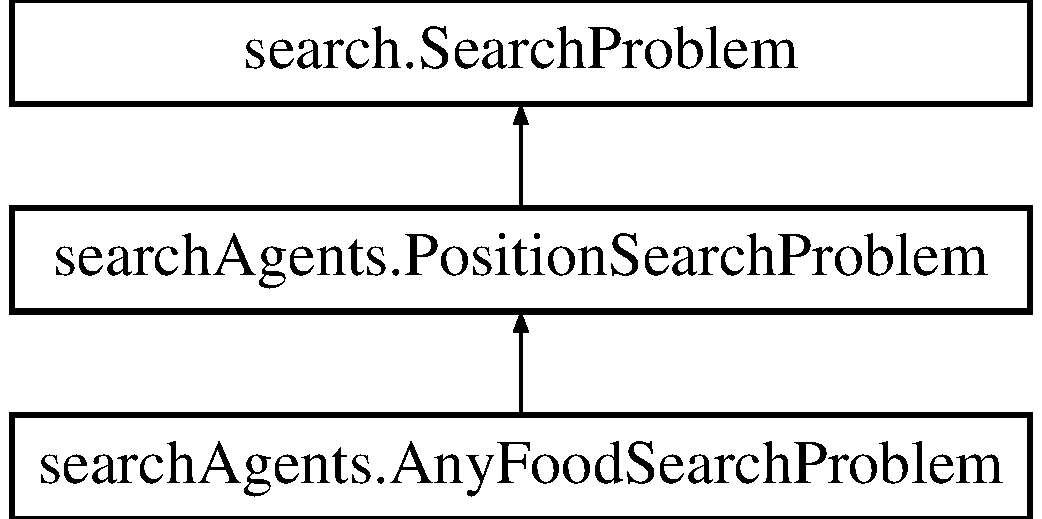
\includegraphics[height=3.000000cm]{classsearch_agents_1_1_position_search_problem}
\end{center}
\end{figure}
\subsection*{Public Member Functions}
\begin{DoxyCompactItemize}
\item 
def \hyperlink{classsearch_agents_1_1_position_search_problem_a59e8c9a64a7b1f994e127f76587145bf}{\+\_\+\+\_\+init\+\_\+\+\_\+} (self, game\+State, cost\+Fn=lambda x\+:1, goal=(1, 1), start=None, warn=True)
\item 
\mbox{\Hypertarget{classsearch_agents_1_1_position_search_problem_a1aacdbd2e27dcc7d1827e9a739c7a67e}\label{classsearch_agents_1_1_position_search_problem_a1aacdbd2e27dcc7d1827e9a739c7a67e}} 
def {\bfseries get\+Start\+State} (self)
\item 
\mbox{\Hypertarget{classsearch_agents_1_1_position_search_problem_abca1168f57dfce26905c037794c483fe}\label{classsearch_agents_1_1_position_search_problem_abca1168f57dfce26905c037794c483fe}} 
def {\bfseries is\+Goal\+State} (self, state)
\item 
def \hyperlink{classsearch_agents_1_1_position_search_problem_a0bdc0dc758b100e61188e2335b763fbf}{get\+Successors} (self, state)
\item 
def \hyperlink{classsearch_agents_1_1_position_search_problem_a31ea791f51f365a42ad8a0030b3a3c5f}{get\+Cost\+Of\+Actions} (self, actions)
\end{DoxyCompactItemize}
\subsection*{Public Attributes}
\begin{DoxyCompactItemize}
\item 
\mbox{\Hypertarget{classsearch_agents_1_1_position_search_problem_ade922b17b94e7612d0e083513c77d92a}\label{classsearch_agents_1_1_position_search_problem_ade922b17b94e7612d0e083513c77d92a}} 
{\bfseries walls}
\item 
\mbox{\Hypertarget{classsearch_agents_1_1_position_search_problem_a5144f1ac0fdeb1cf80a1bb2ecd90b34f}\label{classsearch_agents_1_1_position_search_problem_a5144f1ac0fdeb1cf80a1bb2ecd90b34f}} 
{\bfseries start\+State}
\item 
\mbox{\Hypertarget{classsearch_agents_1_1_position_search_problem_a1d463bd4e4a84e2e9d3a08f8b26c466c}\label{classsearch_agents_1_1_position_search_problem_a1d463bd4e4a84e2e9d3a08f8b26c466c}} 
{\bfseries goal}
\item 
\mbox{\Hypertarget{classsearch_agents_1_1_position_search_problem_a7cd223610ee4fc279273b94856c94bb0}\label{classsearch_agents_1_1_position_search_problem_a7cd223610ee4fc279273b94856c94bb0}} 
{\bfseries cost\+Fn}
\end{DoxyCompactItemize}


\subsection{Detailed Description}
\begin{DoxyVerb}A search problem defines the state space, start state, goal test,
successor function and cost function.  This search problem can be
used to find paths to a particular point on the pacman board.

The state space consists of (x,y) positions in a pacman game.

Note: this search problem is fully specified; you should NOT change it.
\end{DoxyVerb}
 

\subsection{Constructor \& Destructor Documentation}
\mbox{\Hypertarget{classsearch_agents_1_1_position_search_problem_a59e8c9a64a7b1f994e127f76587145bf}\label{classsearch_agents_1_1_position_search_problem_a59e8c9a64a7b1f994e127f76587145bf}} 
\index{search\+Agents\+::\+Position\+Search\+Problem@{search\+Agents\+::\+Position\+Search\+Problem}!\+\_\+\+\_\+init\+\_\+\+\_\+@{\+\_\+\+\_\+init\+\_\+\+\_\+}}
\index{\+\_\+\+\_\+init\+\_\+\+\_\+@{\+\_\+\+\_\+init\+\_\+\+\_\+}!search\+Agents\+::\+Position\+Search\+Problem@{search\+Agents\+::\+Position\+Search\+Problem}}
\subsubsection{\texorpdfstring{\+\_\+\+\_\+init\+\_\+\+\_\+()}{\_\_init\_\_()}}
{\footnotesize\ttfamily def search\+Agents.\+Position\+Search\+Problem.\+\_\+\+\_\+init\+\_\+\+\_\+ (\begin{DoxyParamCaption}\item[{}]{self,  }\item[{}]{game\+State,  }\item[{}]{cost\+Fn = {\ttfamily lambda~x\+:~1},  }\item[{}]{goal = {\ttfamily (1,~1)},  }\item[{}]{start = {\ttfamily None},  }\item[{}]{warn = {\ttfamily True} }\end{DoxyParamCaption})}

\begin{DoxyVerb}Stores the start and goal.

gameState: A GameState object (pacman.py)
costFn: A function from a search state (tuple) to a non-negative number
goal: A position in the gameState
\end{DoxyVerb}
 

\subsection{Member Function Documentation}
\mbox{\Hypertarget{classsearch_agents_1_1_position_search_problem_a31ea791f51f365a42ad8a0030b3a3c5f}\label{classsearch_agents_1_1_position_search_problem_a31ea791f51f365a42ad8a0030b3a3c5f}} 
\index{search\+Agents\+::\+Position\+Search\+Problem@{search\+Agents\+::\+Position\+Search\+Problem}!get\+Cost\+Of\+Actions@{get\+Cost\+Of\+Actions}}
\index{get\+Cost\+Of\+Actions@{get\+Cost\+Of\+Actions}!search\+Agents\+::\+Position\+Search\+Problem@{search\+Agents\+::\+Position\+Search\+Problem}}
\subsubsection{\texorpdfstring{get\+Cost\+Of\+Actions()}{getCostOfActions()}}
{\footnotesize\ttfamily def search\+Agents.\+Position\+Search\+Problem.\+get\+Cost\+Of\+Actions (\begin{DoxyParamCaption}\item[{}]{self,  }\item[{}]{actions }\end{DoxyParamCaption})}

\begin{DoxyVerb}Returns the cost of a particular sequence of actions.  If those actions
include an illegal move, return 999999
\end{DoxyVerb}
 \mbox{\Hypertarget{classsearch_agents_1_1_position_search_problem_a0bdc0dc758b100e61188e2335b763fbf}\label{classsearch_agents_1_1_position_search_problem_a0bdc0dc758b100e61188e2335b763fbf}} 
\index{search\+Agents\+::\+Position\+Search\+Problem@{search\+Agents\+::\+Position\+Search\+Problem}!get\+Successors@{get\+Successors}}
\index{get\+Successors@{get\+Successors}!search\+Agents\+::\+Position\+Search\+Problem@{search\+Agents\+::\+Position\+Search\+Problem}}
\subsubsection{\texorpdfstring{get\+Successors()}{getSuccessors()}}
{\footnotesize\ttfamily def search\+Agents.\+Position\+Search\+Problem.\+get\+Successors (\begin{DoxyParamCaption}\item[{}]{self,  }\item[{}]{state }\end{DoxyParamCaption})}

\begin{DoxyVerb}Returns successor states, the actions they require, and a cost of 1.

 As noted in search.py:
     For a given state, this should return a list of triples,
 (successor, action, stepCost), where 'successor' is a
 successor to the current state, 'action' is the action
 required to get there, and 'stepCost' is the incremental
 cost of expanding to that successor
\end{DoxyVerb}
 

The documentation for this class was generated from the following file\+:\begin{DoxyCompactItemize}
\item 
search\+Agents.\+py\end{DoxyCompactItemize}

\hypertarget{classutil_1_1_priority_queue}{}\section{util.\+Priority\+Queue Class Reference}
\label{classutil_1_1_priority_queue}\index{util.\+Priority\+Queue@{util.\+Priority\+Queue}}
Inheritance diagram for util.\+Priority\+Queue\+:\begin{figure}[H]
\begin{center}
\leavevmode
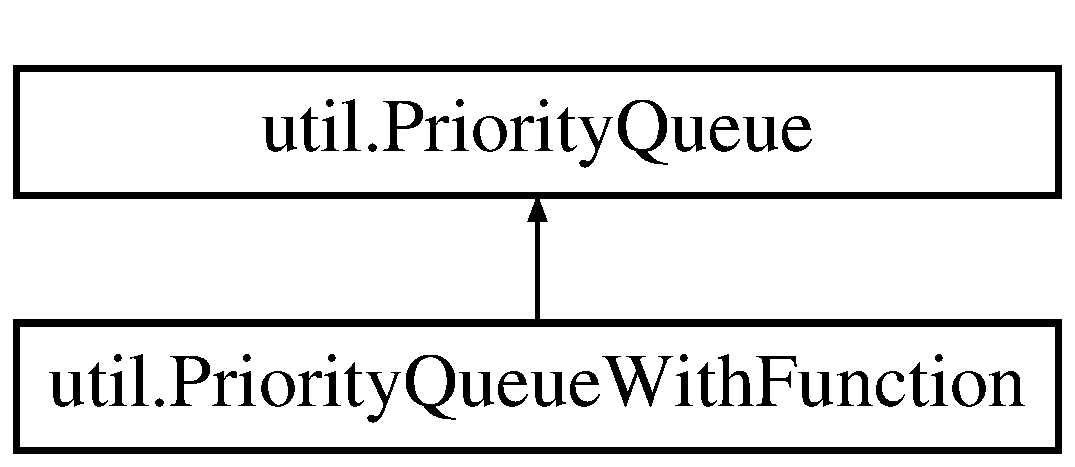
\includegraphics[height=2.000000cm]{classutil_1_1_priority_queue}
\end{center}
\end{figure}
\subsection*{Public Member Functions}
\begin{DoxyCompactItemize}
\item 
\mbox{\Hypertarget{classutil_1_1_priority_queue_a0106af676796b4ebc48d6260867533d9}\label{classutil_1_1_priority_queue_a0106af676796b4ebc48d6260867533d9}} 
def {\bfseries \+\_\+\+\_\+init\+\_\+\+\_\+} (self)
\item 
\mbox{\Hypertarget{classutil_1_1_priority_queue_a57a348c6571b80ac89d401af27c9bb31}\label{classutil_1_1_priority_queue_a57a348c6571b80ac89d401af27c9bb31}} 
def {\bfseries push} (self, item, priority)
\item 
\mbox{\Hypertarget{classutil_1_1_priority_queue_a7bfd9bfe51ecada957b3bb69c638e41c}\label{classutil_1_1_priority_queue_a7bfd9bfe51ecada957b3bb69c638e41c}} 
def {\bfseries pop} (self)
\item 
\mbox{\Hypertarget{classutil_1_1_priority_queue_a7e9393829a3f71d06be25595e80c7be9}\label{classutil_1_1_priority_queue_a7e9393829a3f71d06be25595e80c7be9}} 
def {\bfseries is\+Empty} (self)
\end{DoxyCompactItemize}
\subsection*{Public Attributes}
\begin{DoxyCompactItemize}
\item 
\mbox{\Hypertarget{classutil_1_1_priority_queue_a06389a4f3b391e387758f633c15950e8}\label{classutil_1_1_priority_queue_a06389a4f3b391e387758f633c15950e8}} 
{\bfseries heap}
\end{DoxyCompactItemize}


\subsection{Detailed Description}
\begin{DoxyVerb}  Implements a priority queue data structure. Each inserted item
  has a priority associated with it and the client is usually interested
  in quick retrieval of the lowest-priority item in the queue. This
  data structure allows O(1) access to the lowest-priority item.
  
  Note that this PriorityQueue does not allow you to change the priority
  of an item.  However, you may insert the same item multiple times with
  different priorities.
\end{DoxyVerb}
 

The documentation for this class was generated from the following file\+:\begin{DoxyCompactItemize}
\item 
util.\+py\end{DoxyCompactItemize}

\hypertarget{classutil_1_1_priority_queue_with_function}{}\section{util.\+Priority\+Queue\+With\+Function Class Reference}
\label{classutil_1_1_priority_queue_with_function}\index{util.\+Priority\+Queue\+With\+Function@{util.\+Priority\+Queue\+With\+Function}}
Inheritance diagram for util.\+Priority\+Queue\+With\+Function\+:\begin{figure}[H]
\begin{center}
\leavevmode
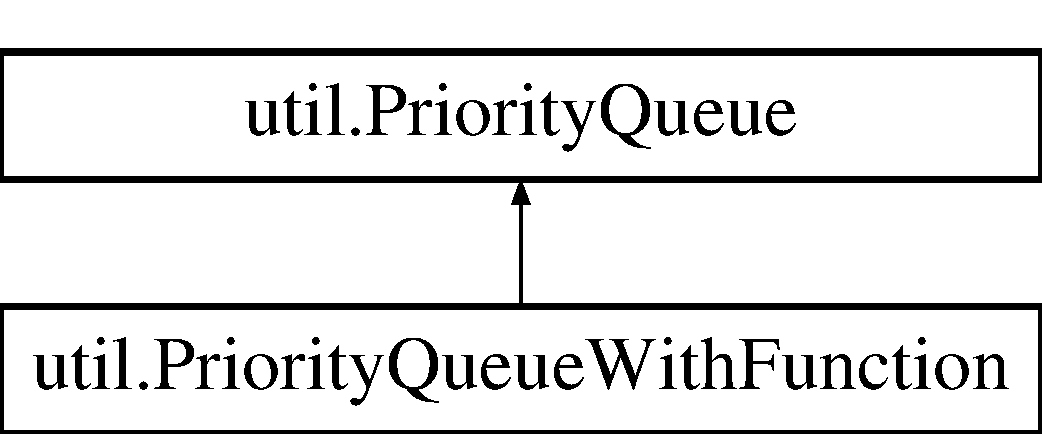
\includegraphics[height=2.000000cm]{classutil_1_1_priority_queue_with_function}
\end{center}
\end{figure}
\subsection*{Public Member Functions}
\begin{DoxyCompactItemize}
\item 
\mbox{\Hypertarget{classutil_1_1_priority_queue_with_function_a27ea0d044a098275fb4156ac4e35fcc2}\label{classutil_1_1_priority_queue_with_function_a27ea0d044a098275fb4156ac4e35fcc2}} 
def {\bfseries \+\_\+\+\_\+init\+\_\+\+\_\+} (self, priority\+Function)
\item 
\mbox{\Hypertarget{classutil_1_1_priority_queue_with_function_ababfbf747ff01219b5e03b06f7f30544}\label{classutil_1_1_priority_queue_with_function_ababfbf747ff01219b5e03b06f7f30544}} 
def {\bfseries push} (self, item)
\end{DoxyCompactItemize}
\subsection*{Public Attributes}
\begin{DoxyCompactItemize}
\item 
\mbox{\Hypertarget{classutil_1_1_priority_queue_with_function_a596184d513305b42e0a7a05f75fd7108}\label{classutil_1_1_priority_queue_with_function_a596184d513305b42e0a7a05f75fd7108}} 
{\bfseries priority\+Function}
\end{DoxyCompactItemize}


\subsection{Detailed Description}
\begin{DoxyVerb}Implements a priority queue with the same push/pop signature of the
Queue and the Stack classes. This is designed for drop-in replacement for
those two classes. The caller has to provide a priority function, which
extracts each item's priority.
\end{DoxyVerb}
 

The documentation for this class was generated from the following file\+:\begin{DoxyCompactItemize}
\item 
util.\+py\end{DoxyCompactItemize}

\hypertarget{classutil_1_1_queue}{}\section{util.\+Queue Class Reference}
\label{classutil_1_1_queue}\index{util.\+Queue@{util.\+Queue}}
\subsection*{Public Member Functions}
\begin{DoxyCompactItemize}
\item 
\mbox{\Hypertarget{classutil_1_1_queue_a65b116b07123e34eef3f210504565f78}\label{classutil_1_1_queue_a65b116b07123e34eef3f210504565f78}} 
def {\bfseries \+\_\+\+\_\+init\+\_\+\+\_\+} (self)
\item 
\mbox{\Hypertarget{classutil_1_1_queue_acf2bffae0b1b8b663a7489ba4fd51d3a}\label{classutil_1_1_queue_acf2bffae0b1b8b663a7489ba4fd51d3a}} 
def {\bfseries push} (self, item)
\item 
def \hyperlink{classutil_1_1_queue_acb244571d931f24864b4a2e889130396}{pop} (self)
\item 
\mbox{\Hypertarget{classutil_1_1_queue_aacf6d8d4ee520c2f5209e4740f6419af}\label{classutil_1_1_queue_aacf6d8d4ee520c2f5209e4740f6419af}} 
def {\bfseries is\+Empty} (self)
\end{DoxyCompactItemize}
\subsection*{Public Attributes}
\begin{DoxyCompactItemize}
\item 
\mbox{\Hypertarget{classutil_1_1_queue_ac25f813a4fc57ebd0e687ab845df3bbd}\label{classutil_1_1_queue_ac25f813a4fc57ebd0e687ab845df3bbd}} 
{\bfseries list}
\end{DoxyCompactItemize}


\subsection{Member Function Documentation}
\mbox{\Hypertarget{classutil_1_1_queue_acb244571d931f24864b4a2e889130396}\label{classutil_1_1_queue_acb244571d931f24864b4a2e889130396}} 
\index{util\+::\+Queue@{util\+::\+Queue}!pop@{pop}}
\index{pop@{pop}!util\+::\+Queue@{util\+::\+Queue}}
\subsubsection{\texorpdfstring{pop()}{pop()}}
{\footnotesize\ttfamily def util.\+Queue.\+pop (\begin{DoxyParamCaption}\item[{}]{self }\end{DoxyParamCaption})}

\begin{DoxyVerb}  Dequeue the earliest enqueued item still in the queue. This
  operation removes the item from the queue.
\end{DoxyVerb}
 

The documentation for this class was generated from the following file\+:\begin{DoxyCompactItemize}
\item 
util.\+py\end{DoxyCompactItemize}

\hypertarget{classghost_agents_1_1_random_ghost}{}\section{ghost\+Agents.\+Random\+Ghost Class Reference}
\label{classghost_agents_1_1_random_ghost}\index{ghost\+Agents.\+Random\+Ghost@{ghost\+Agents.\+Random\+Ghost}}
Inheritance diagram for ghost\+Agents.\+Random\+Ghost\+:\begin{figure}[H]
\begin{center}
\leavevmode
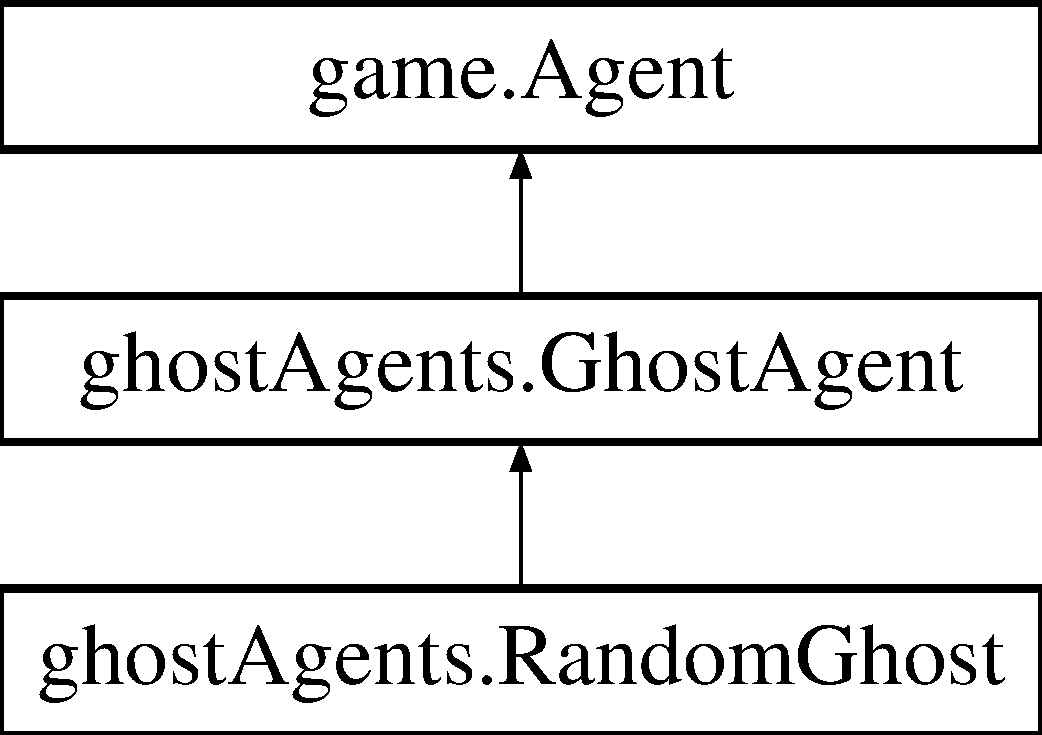
\includegraphics[height=3.000000cm]{classghost_agents_1_1_random_ghost}
\end{center}
\end{figure}
\subsection*{Public Member Functions}
\begin{DoxyCompactItemize}
\item 
\mbox{\Hypertarget{classghost_agents_1_1_random_ghost_a4ff85a0f0b0c82b2c80021470d6d6f25}\label{classghost_agents_1_1_random_ghost_a4ff85a0f0b0c82b2c80021470d6d6f25}} 
def {\bfseries get\+Distribution} (self, state)
\end{DoxyCompactItemize}
\subsection*{Additional Inherited Members}


The documentation for this class was generated from the following file\+:\begin{DoxyCompactItemize}
\item 
ghost\+Agents.\+py\end{DoxyCompactItemize}

\hypertarget{classsearch_agents_1_1_search_agent}{}\section{search\+Agents.\+Search\+Agent Class Reference}
\label{classsearch_agents_1_1_search_agent}\index{search\+Agents.\+Search\+Agent@{search\+Agents.\+Search\+Agent}}
Inheritance diagram for search\+Agents.\+Search\+Agent\+:\begin{figure}[H]
\begin{center}
\leavevmode
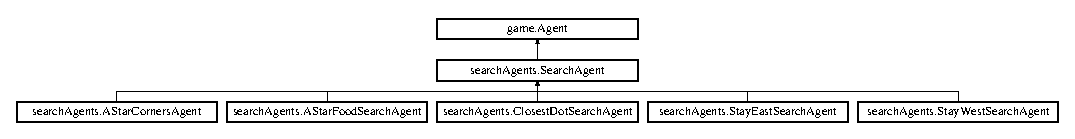
\includegraphics[height=1.417722cm]{classsearch_agents_1_1_search_agent}
\end{center}
\end{figure}
\subsection*{Public Member Functions}
\begin{DoxyCompactItemize}
\item 
\mbox{\Hypertarget{classsearch_agents_1_1_search_agent_ace72a2a8f3cd7baa33341b58d098f0a9}\label{classsearch_agents_1_1_search_agent_ace72a2a8f3cd7baa33341b58d098f0a9}} 
def {\bfseries \+\_\+\+\_\+init\+\_\+\+\_\+} (self, fn=\textquotesingle{}depth\+First\+Search\textquotesingle{}, prob=\textquotesingle{}\hyperlink{classsearch_agents_1_1_position_search_problem}{Position\+Search\+Problem}\textquotesingle{}, heuristic=\textquotesingle{}null\+Heuristic\textquotesingle{})
\item 
def \hyperlink{classsearch_agents_1_1_search_agent_ab6fba6e09d2d604f1f1f403dc41ecfcc}{register\+Initial\+State} (self, state)
\item 
def \hyperlink{classsearch_agents_1_1_search_agent_a93ab497b5d38054a8aa628c2a2339d13}{get\+Action} (self, state)
\end{DoxyCompactItemize}
\subsection*{Public Attributes}
\begin{DoxyCompactItemize}
\item 
\mbox{\Hypertarget{classsearch_agents_1_1_search_agent_a0069fcdd1ef320fba53b061a089b8c75}\label{classsearch_agents_1_1_search_agent_a0069fcdd1ef320fba53b061a089b8c75}} 
{\bfseries search\+Function}
\item 
\mbox{\Hypertarget{classsearch_agents_1_1_search_agent_aefb34eff1833b65182b9b02fe1f3e91c}\label{classsearch_agents_1_1_search_agent_aefb34eff1833b65182b9b02fe1f3e91c}} 
{\bfseries search\+Type}
\item 
\mbox{\Hypertarget{classsearch_agents_1_1_search_agent_a9c62e2023013bf42e0fa859ba7eab71d}\label{classsearch_agents_1_1_search_agent_a9c62e2023013bf42e0fa859ba7eab71d}} 
{\bfseries actions}
\item 
\mbox{\Hypertarget{classsearch_agents_1_1_search_agent_aa38beac5831e0bdab8445d0d792c684c}\label{classsearch_agents_1_1_search_agent_aa38beac5831e0bdab8445d0d792c684c}} 
{\bfseries action\+Index}
\end{DoxyCompactItemize}


\subsection{Detailed Description}
\begin{DoxyVerb}This very general search agent finds a path using a supplied search algorithm for a
supplied search problem, then returns actions to follow that path.

As a default, this agent runs DFS on a PositionSearchProblem to find location (1,1)

Options for fn include:
  depthFirstSearch or dfs
  breadthFirstSearch or bfs


Note: You should NOT change any code in SearchAgent
\end{DoxyVerb}
 

\subsection{Member Function Documentation}
\mbox{\Hypertarget{classsearch_agents_1_1_search_agent_a93ab497b5d38054a8aa628c2a2339d13}\label{classsearch_agents_1_1_search_agent_a93ab497b5d38054a8aa628c2a2339d13}} 
\index{search\+Agents\+::\+Search\+Agent@{search\+Agents\+::\+Search\+Agent}!get\+Action@{get\+Action}}
\index{get\+Action@{get\+Action}!search\+Agents\+::\+Search\+Agent@{search\+Agents\+::\+Search\+Agent}}
\subsubsection{\texorpdfstring{get\+Action()}{getAction()}}
{\footnotesize\ttfamily def search\+Agents.\+Search\+Agent.\+get\+Action (\begin{DoxyParamCaption}\item[{}]{self,  }\item[{}]{state }\end{DoxyParamCaption})}

\begin{DoxyVerb}Returns the next action in the path chosen earlier (in registerInitialState).  Return
Directions.STOP if there is no further action to take.

state: a GameState object (pacman.py)
\end{DoxyVerb}
 \mbox{\Hypertarget{classsearch_agents_1_1_search_agent_ab6fba6e09d2d604f1f1f403dc41ecfcc}\label{classsearch_agents_1_1_search_agent_ab6fba6e09d2d604f1f1f403dc41ecfcc}} 
\index{search\+Agents\+::\+Search\+Agent@{search\+Agents\+::\+Search\+Agent}!register\+Initial\+State@{register\+Initial\+State}}
\index{register\+Initial\+State@{register\+Initial\+State}!search\+Agents\+::\+Search\+Agent@{search\+Agents\+::\+Search\+Agent}}
\subsubsection{\texorpdfstring{register\+Initial\+State()}{registerInitialState()}}
{\footnotesize\ttfamily def search\+Agents.\+Search\+Agent.\+register\+Initial\+State (\begin{DoxyParamCaption}\item[{}]{self,  }\item[{}]{state }\end{DoxyParamCaption})}

\begin{DoxyVerb}This is the first time that the agent sees the layout of the game board. Here, we
choose a path to the goal.  In this phase, the agent should compute the path to the
goal and store it in a local variable.  All of the work is done in this method!

state: a GameState object (pacman.py)
\end{DoxyVerb}
 

The documentation for this class was generated from the following file\+:\begin{DoxyCompactItemize}
\item 
search\+Agents.\+py\end{DoxyCompactItemize}

\hypertarget{classsearch_1_1_search_problem}{}\section{search.\+Search\+Problem Class Reference}
\label{classsearch_1_1_search_problem}\index{search.\+Search\+Problem@{search.\+Search\+Problem}}
Inheritance diagram for search.\+Search\+Problem\+:\begin{figure}[H]
\begin{center}
\leavevmode
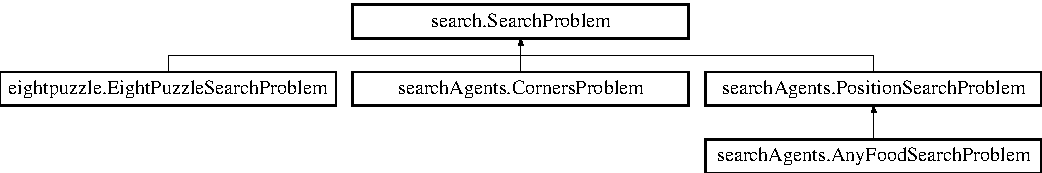
\includegraphics[height=2.323651cm]{classsearch_1_1_search_problem}
\end{center}
\end{figure}
\subsection*{Public Member Functions}
\begin{DoxyCompactItemize}
\item 
def \hyperlink{classsearch_1_1_search_problem_a4ffd125695767220d899c77f058e7577}{get\+Start\+State} (self)
\item 
def \hyperlink{classsearch_1_1_search_problem_ac856fffa6ab38abe071bde684b84b148}{is\+Goal\+State} (self, state)
\item 
def \hyperlink{classsearch_1_1_search_problem_a2e97eaf1f2b9fcb129711a862a4ebd63}{get\+Successors} (self, state)
\item 
def \hyperlink{classsearch_1_1_search_problem_a444a40c5ac6947d7ef35408f34690a1a}{get\+Cost\+Of\+Actions} (self, actions)
\end{DoxyCompactItemize}


\subsection{Detailed Description}
\begin{DoxyVerb}This class outlines the structure of a search problem, but doesn't implement
any of the methods (in object-oriented terminology: an abstract class).

You do not need to change anything in this class, ever.
\end{DoxyVerb}
 

\subsection{Member Function Documentation}
\mbox{\Hypertarget{classsearch_1_1_search_problem_a444a40c5ac6947d7ef35408f34690a1a}\label{classsearch_1_1_search_problem_a444a40c5ac6947d7ef35408f34690a1a}} 
\index{search\+::\+Search\+Problem@{search\+::\+Search\+Problem}!get\+Cost\+Of\+Actions@{get\+Cost\+Of\+Actions}}
\index{get\+Cost\+Of\+Actions@{get\+Cost\+Of\+Actions}!search\+::\+Search\+Problem@{search\+::\+Search\+Problem}}
\subsubsection{\texorpdfstring{get\+Cost\+Of\+Actions()}{getCostOfActions()}}
{\footnotesize\ttfamily def search.\+Search\+Problem.\+get\+Cost\+Of\+Actions (\begin{DoxyParamCaption}\item[{}]{self,  }\item[{}]{actions }\end{DoxyParamCaption})}

\begin{DoxyVerb} actions: A list of actions to take

This method returns the total cost of a particular sequence of actions.  The sequence must
be composed of legal moves
\end{DoxyVerb}
 \mbox{\Hypertarget{classsearch_1_1_search_problem_a4ffd125695767220d899c77f058e7577}\label{classsearch_1_1_search_problem_a4ffd125695767220d899c77f058e7577}} 
\index{search\+::\+Search\+Problem@{search\+::\+Search\+Problem}!get\+Start\+State@{get\+Start\+State}}
\index{get\+Start\+State@{get\+Start\+State}!search\+::\+Search\+Problem@{search\+::\+Search\+Problem}}
\subsubsection{\texorpdfstring{get\+Start\+State()}{getStartState()}}
{\footnotesize\ttfamily def search.\+Search\+Problem.\+get\+Start\+State (\begin{DoxyParamCaption}\item[{}]{self }\end{DoxyParamCaption})}

\begin{DoxyVerb}Returns the start state for the search problem
\end{DoxyVerb}
 \mbox{\Hypertarget{classsearch_1_1_search_problem_a2e97eaf1f2b9fcb129711a862a4ebd63}\label{classsearch_1_1_search_problem_a2e97eaf1f2b9fcb129711a862a4ebd63}} 
\index{search\+::\+Search\+Problem@{search\+::\+Search\+Problem}!get\+Successors@{get\+Successors}}
\index{get\+Successors@{get\+Successors}!search\+::\+Search\+Problem@{search\+::\+Search\+Problem}}
\subsubsection{\texorpdfstring{get\+Successors()}{getSuccessors()}}
{\footnotesize\ttfamily def search.\+Search\+Problem.\+get\+Successors (\begin{DoxyParamCaption}\item[{}]{self,  }\item[{}]{state }\end{DoxyParamCaption})}

\begin{DoxyVerb}  state: Search state

For a given state, this should return a list of triples,
(successor, action, stepCost), where 'successor' is a
successor to the current state, 'action' is the action
required to get there, and 'stepCost' is the incremental
cost of expanding to that successor
\end{DoxyVerb}
 \mbox{\Hypertarget{classsearch_1_1_search_problem_ac856fffa6ab38abe071bde684b84b148}\label{classsearch_1_1_search_problem_ac856fffa6ab38abe071bde684b84b148}} 
\index{search\+::\+Search\+Problem@{search\+::\+Search\+Problem}!is\+Goal\+State@{is\+Goal\+State}}
\index{is\+Goal\+State@{is\+Goal\+State}!search\+::\+Search\+Problem@{search\+::\+Search\+Problem}}
\subsubsection{\texorpdfstring{is\+Goal\+State()}{isGoalState()}}
{\footnotesize\ttfamily def search.\+Search\+Problem.\+is\+Goal\+State (\begin{DoxyParamCaption}\item[{}]{self,  }\item[{}]{state }\end{DoxyParamCaption})}

\begin{DoxyVerb}  state: Search state

Returns True if and only if the state is a valid goal state
\end{DoxyVerb}
 

The documentation for this class was generated from the following file\+:\begin{DoxyCompactItemize}
\item 
search.\+py\end{DoxyCompactItemize}

\hypertarget{classutil_1_1_stack}{}\section{util.\+Stack Class Reference}
\label{classutil_1_1_stack}\index{util.\+Stack@{util.\+Stack}}
\subsection*{Public Member Functions}
\begin{DoxyCompactItemize}
\item 
\mbox{\Hypertarget{classutil_1_1_stack_a33ce3c769ea27fa11e4c924b79f221cf}\label{classutil_1_1_stack_a33ce3c769ea27fa11e4c924b79f221cf}} 
def {\bfseries \+\_\+\+\_\+init\+\_\+\+\_\+} (self)
\item 
\mbox{\Hypertarget{classutil_1_1_stack_a6f20aecd317c195f98e86b61c1756f3d}\label{classutil_1_1_stack_a6f20aecd317c195f98e86b61c1756f3d}} 
def {\bfseries push} (self, item)
\item 
\mbox{\Hypertarget{classutil_1_1_stack_a3e09e2fd824f1a710fb1bfa76dc58abe}\label{classutil_1_1_stack_a3e09e2fd824f1a710fb1bfa76dc58abe}} 
def {\bfseries pop} (self)
\item 
\mbox{\Hypertarget{classutil_1_1_stack_a1ea38d74b69c02ce0946e9104824beea}\label{classutil_1_1_stack_a1ea38d74b69c02ce0946e9104824beea}} 
def {\bfseries is\+Empty} (self)
\end{DoxyCompactItemize}
\subsection*{Public Attributes}
\begin{DoxyCompactItemize}
\item 
\mbox{\Hypertarget{classutil_1_1_stack_ae8fb89dd9d2961cc72c6cbfc3135ad1a}\label{classutil_1_1_stack_ae8fb89dd9d2961cc72c6cbfc3135ad1a}} 
{\bfseries list}
\end{DoxyCompactItemize}


The documentation for this class was generated from the following file\+:\begin{DoxyCompactItemize}
\item 
util.\+py\end{DoxyCompactItemize}

\hypertarget{classsearch_agents_1_1_stay_east_search_agent}{}\section{search\+Agents.\+Stay\+East\+Search\+Agent Class Reference}
\label{classsearch_agents_1_1_stay_east_search_agent}\index{search\+Agents.\+Stay\+East\+Search\+Agent@{search\+Agents.\+Stay\+East\+Search\+Agent}}
Inheritance diagram for search\+Agents.\+Stay\+East\+Search\+Agent\+:\begin{figure}[H]
\begin{center}
\leavevmode
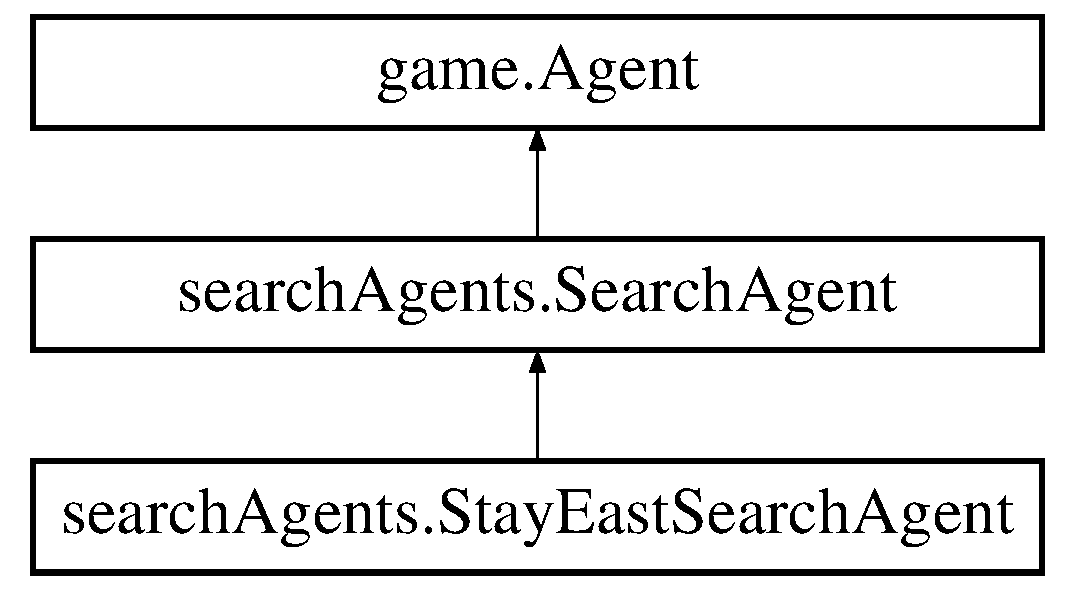
\includegraphics[height=3.000000cm]{classsearch_agents_1_1_stay_east_search_agent}
\end{center}
\end{figure}
\subsection*{Public Member Functions}
\begin{DoxyCompactItemize}
\item 
\mbox{\Hypertarget{classsearch_agents_1_1_stay_east_search_agent_a43052b0d7816b831021ddfd048f6c6e8}\label{classsearch_agents_1_1_stay_east_search_agent_a43052b0d7816b831021ddfd048f6c6e8}} 
def {\bfseries \+\_\+\+\_\+init\+\_\+\+\_\+} (self)
\end{DoxyCompactItemize}
\subsection*{Public Attributes}
\begin{DoxyCompactItemize}
\item 
\mbox{\Hypertarget{classsearch_agents_1_1_stay_east_search_agent_aded2367f9cbc220937cae300a95c56e8}\label{classsearch_agents_1_1_stay_east_search_agent_aded2367f9cbc220937cae300a95c56e8}} 
{\bfseries search\+Function}
\item 
\mbox{\Hypertarget{classsearch_agents_1_1_stay_east_search_agent_a5fe9d6f2edc6fc40df1492b22bfb3869}\label{classsearch_agents_1_1_stay_east_search_agent_a5fe9d6f2edc6fc40df1492b22bfb3869}} 
{\bfseries search\+Type}
\end{DoxyCompactItemize}


\subsection{Detailed Description}
\begin{DoxyVerb}An agent for position search with a cost function that penalizes being in
positions on the West side of the board.

The cost function for stepping into a position (x,y) is 1/2^x.
\end{DoxyVerb}
 

The documentation for this class was generated from the following file\+:\begin{DoxyCompactItemize}
\item 
search\+Agents.\+py\end{DoxyCompactItemize}

\hypertarget{classsearch_agents_1_1_stay_west_search_agent}{}\section{search\+Agents.\+Stay\+West\+Search\+Agent Class Reference}
\label{classsearch_agents_1_1_stay_west_search_agent}\index{search\+Agents.\+Stay\+West\+Search\+Agent@{search\+Agents.\+Stay\+West\+Search\+Agent}}
Inheritance diagram for search\+Agents.\+Stay\+West\+Search\+Agent\+:\begin{figure}[H]
\begin{center}
\leavevmode
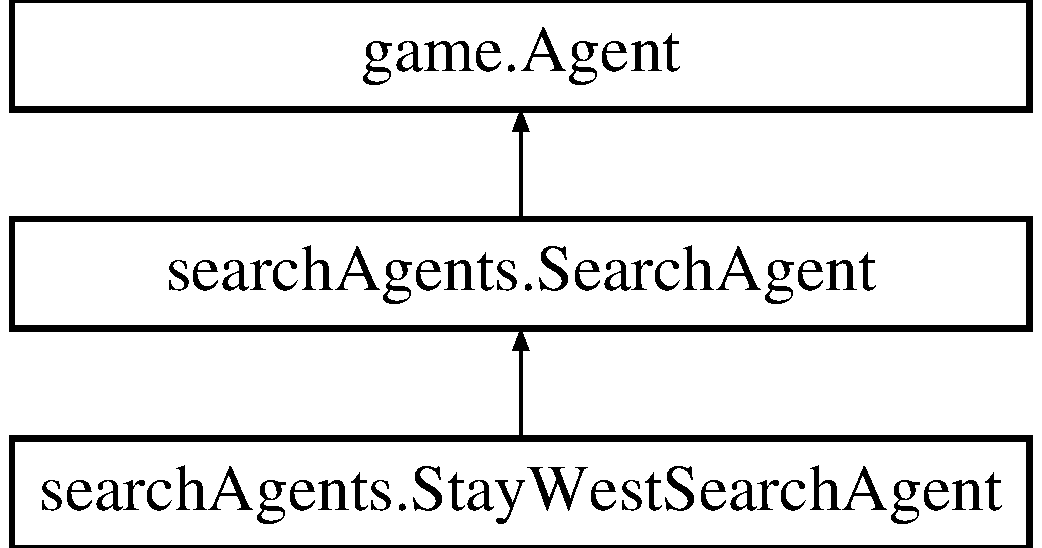
\includegraphics[height=3.000000cm]{classsearch_agents_1_1_stay_west_search_agent}
\end{center}
\end{figure}
\subsection*{Public Member Functions}
\begin{DoxyCompactItemize}
\item 
\mbox{\Hypertarget{classsearch_agents_1_1_stay_west_search_agent_a2a222b3493fff4cc26f4705a926ce580}\label{classsearch_agents_1_1_stay_west_search_agent_a2a222b3493fff4cc26f4705a926ce580}} 
def {\bfseries \+\_\+\+\_\+init\+\_\+\+\_\+} (self)
\end{DoxyCompactItemize}
\subsection*{Public Attributes}
\begin{DoxyCompactItemize}
\item 
\mbox{\Hypertarget{classsearch_agents_1_1_stay_west_search_agent_ac44b94be3b7571440773fb38899ce6db}\label{classsearch_agents_1_1_stay_west_search_agent_ac44b94be3b7571440773fb38899ce6db}} 
{\bfseries search\+Function}
\item 
\mbox{\Hypertarget{classsearch_agents_1_1_stay_west_search_agent_a5d1b6647ecf29ab11a779da574ff327c}\label{classsearch_agents_1_1_stay_west_search_agent_a5d1b6647ecf29ab11a779da574ff327c}} 
{\bfseries search\+Type}
\end{DoxyCompactItemize}


\subsection{Detailed Description}
\begin{DoxyVerb}An agent for position search with a cost function that penalizes being in
positions on the East side of the board.

The cost function for stepping into a position (x,y) is 2^x.
\end{DoxyVerb}
 

The documentation for this class was generated from the following file\+:\begin{DoxyCompactItemize}
\item 
search\+Agents.\+py\end{DoxyCompactItemize}

\hypertarget{classutil_1_1_timeout_function}{}\section{util.\+Timeout\+Function Class Reference}
\label{classutil_1_1_timeout_function}\index{util.\+Timeout\+Function@{util.\+Timeout\+Function}}
\subsection*{Public Member Functions}
\begin{DoxyCompactItemize}
\item 
\mbox{\Hypertarget{classutil_1_1_timeout_function_a6cba9d2d064cd8fb00fb8c281d174eff}\label{classutil_1_1_timeout_function_a6cba9d2d064cd8fb00fb8c281d174eff}} 
def {\bfseries \+\_\+\+\_\+init\+\_\+\+\_\+} (self, function, timeout)
\item 
\mbox{\Hypertarget{classutil_1_1_timeout_function_aa7f7a6b73e2aaa4659197fb6feba9e1c}\label{classutil_1_1_timeout_function_aa7f7a6b73e2aaa4659197fb6feba9e1c}} 
def {\bfseries handle\+\_\+timeout} (self, signum, frame)
\item 
\mbox{\Hypertarget{classutil_1_1_timeout_function_a59209385cbe2cb4bfd5c488a51404051}\label{classutil_1_1_timeout_function_a59209385cbe2cb4bfd5c488a51404051}} 
def {\bfseries \+\_\+\+\_\+call\+\_\+\+\_\+} (self, args)
\end{DoxyCompactItemize}
\subsection*{Public Attributes}
\begin{DoxyCompactItemize}
\item 
\mbox{\Hypertarget{classutil_1_1_timeout_function_a4cbbcc8ad43fc8e2a5665a76178bc3aa}\label{classutil_1_1_timeout_function_a4cbbcc8ad43fc8e2a5665a76178bc3aa}} 
{\bfseries timeout}
\item 
\mbox{\Hypertarget{classutil_1_1_timeout_function_ac969bf0077874d36f87e2aba1628b664}\label{classutil_1_1_timeout_function_ac969bf0077874d36f87e2aba1628b664}} 
{\bfseries function}
\end{DoxyCompactItemize}


The documentation for this class was generated from the following file\+:\begin{DoxyCompactItemize}
\item 
util.\+py\end{DoxyCompactItemize}

\hypertarget{classutil_1_1_timeout_function_exception}{}\section{util.\+Timeout\+Function\+Exception Class Reference}
\label{classutil_1_1_timeout_function_exception}\index{util.\+Timeout\+Function\+Exception@{util.\+Timeout\+Function\+Exception}}
Inheritance diagram for util.\+Timeout\+Function\+Exception\+:\begin{figure}[H]
\begin{center}
\leavevmode
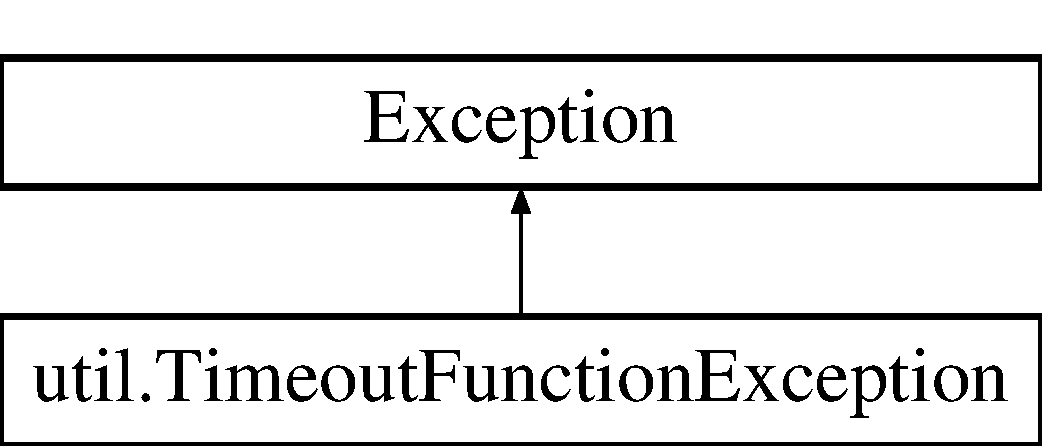
\includegraphics[height=2.000000cm]{classutil_1_1_timeout_function_exception}
\end{center}
\end{figure}


\subsection{Detailed Description}
\begin{DoxyVerb}Exception to raise on a timeout\end{DoxyVerb}
 

The documentation for this class was generated from the following file\+:\begin{DoxyCompactItemize}
\item 
util.\+py\end{DoxyCompactItemize}

%--- End generated contents ---

% Index
\backmatter
\newpage
\phantomsection
\clearemptydoublepage
\addcontentsline{toc}{chapter}{Index}
\printindex

\end{document}
